
%Generazione delle variabili che andranno a sostituire quelle del template 'HomePage'
\newcommand{\documento}{\AdR}
\newcommand{\nomedocumentofisico}{\AdRv.pdf}
\newcommand{\redazione}{\CV \\ & \NC}
\newcommand{\verifica}{\MM \\ & \TG}
\newcommand{\versione}{1.0.0}
\newcommand{\approvazione}{\SG}
\newcommand{\uso}{Esterno}
\newcommand{\datacreazione}{27 novembre 2018} 
\newcommand{\datamodifica}{04 marzo 2019}
\newcommand{\stato}{Approvato}
\newcommand{\destinateTo}{\TV, \\ & \RC, \\ & \II}

\def\TABELLE{true} % abilita - disabilita l'indice delle tabelle
\def\FIGURE{true}  % abilita - disabilita l'indice delle figure

\documentclass[a4paper,11pt]{article}

\usepackage{ifthen}
\usepackage[english,italian]{babel}
\usepackage[utf8]{inputenc}
\usepackage[T1]{fontenc}
\usepackage{float}
\usepackage{chapterbib}
\usepackage{graphicx}
\usepackage[a4paper,top=2.5cm,bottom=2.5cm,left=2.5cm,right=2.5cm]{geometry}

\PassOptionsToPackage{hyphens}{url}\usepackage[hyperfootnotes=false]{hyperref}
\hypersetup{%
	colorlinks=true,
	citecolor=black,
	linkcolor=black,
	urlcolor=blue
}

\usepackage{enumitem}
\usepackage{eurosym}
\usepackage{booktabs}
\usepackage{fancyhdr}
\usepackage{totpages}
\usepackage{tabularx, array}
\usepackage{dcolumn}
\usepackage{epstopdf}
\usepackage{booktabs}
\usepackage{fancyhdr}
\usepackage{longtable}
\usepackage{calc}
\usepackage{datatool}
\usepackage[bottom]{footmisc}
\usepackage{listings}
\usepackage{textcomp}
\usepackage{titlesec}
\usepackage{rotating}
\usepackage{multirow}
\usepackage{placeins}
\usepackage{color}
\usepackage{makecell}
\usepackage{lscape}
 
\usepackage[table,usenames,dvipsnames]{xcolor}
% Definizione di nuovi colori da poter usare per le tabelle
\definecolor{lightgray}{gray}{0.92}
\definecolor{lightblue}{rgb}{0.93,0.95,1.0}
\definecolor{headgray}{gray}{0.88}

% Ridefinizione dell'env tabularx. Il vecchio è utilizzabile con l'env oldtabularx
\let\oldtabularx\tabularx
\let\endoldtabularx\endtabularx
\renewenvironment{tabularx}{\rowcolors{2}{white}{lightgray}\oldtabularx}{\endoldtabularx}

% Per tabularx con padding, parametro tra [], eg [1.3]
\newenvironment{paddedtablex}[1][1]{%
	\renewcommand*{\arraystretch}{#1}%
	\renewcommand\theadfont{\bfseries}%
	\tabularx%
}{%
	\endtabularx
}

% Ridefinizione dell'env tabular. Il vecchio è utilizzabile con l'env oldtabular
\let\oldtabular\tabular
\let\endoldtabular\endtabular
\renewenvironment{tabular}{\rowcolors{2}{lightgray}{white}\oldtabular}{\endoldtabular}

% Per tabular con padding, parametro tra [], eg [1.3]
\newenvironment{paddedtable}[1][1]{%
	\renewcommand*{\arraystretch}{#1}%
	\renewcommand\theadfont{\bfseries}%
	\tabular%
}{%
	\endtabular
}

% ***TABELLA ANALISI RISCHI PDP***

\newenvironment{risktable}[1][1]{%
	\centering%
	\renewcommand*{\arraystretch}{1.4}%
	\renewcommand\theadfont{\bfseries}%
	\oldtabularx%
}{%
	\endoldtabularx
}

% ***TABELLA SUDDIVISIONE DEL LAVORO PDP***

\newenvironment{detailtable}[1][1]{%
	\centering%
	\renewcommand*{\arraystretch}{1.4}%
	\renewcommand\theadfont{\bfseries}%
	\oldtabularx%
}{%
	\endoldtabularx
}

% ***TABELLA ORGANIGRAMMA***

\newenvironment{orgtable}[1][1]{%
	\centering%
	\renewcommand*{\arraystretch}{1.4}%
	\renewcommand\theadfont{\bfseries}%
	\oldtabularx%
}{%
	\endoldtabularx
}


% DA SPOSTARE SU COMANDI
% ***DOUBLE LINE***

\def\mydoublerule#1#2#3{%%
	\hrule width#1 height#2 \vskip#2
	\hrule width#1 height#3 
}

% ***NUOVO TIPO DI CELLA CENTRATA***

\newcolumntype{Y}{>{\centering\arraybackslash}X}

% ***STILE PAGINA***
\pagestyle{fancy}

% ***INTESTAZIONE***
\rhead{\Large{\progetto} \\ \footnotesize{\documento}}
\lhead{
\includegraphics[keepaspectratio = true, width = 25px]{../template/icons/a6(1).png}}

% ***PIÈ DI PAGINA***
\lfoot{\textit{\gruppo} \\
\footnotesize{\email}}

\rfoot{\thepage} % per le prime pagine: mostra solo il numero romano
\cfoot{}
\renewcommand{\footrulewidth}{0.4pt}   % Linea sopra il piè di pagina
\renewcommand{\headrulewidth}{0.4pt}  % Linea sotto l'intestazione

% ***INSERIMENTO DI NUOVE SOTTOSEZIONI
\setcounter{secnumdepth}{7} %mostra nel documento fino al livello 8 (1.2.3.4.5.6.7.8)
\setcounter{tocdepth}{7}    % mostra nell'indice fino al livello 8 (1.2.3.4.5.6.7.8)


\makeatletter
\newcounter{subsubparagraph}[subparagraph]
\renewcommand\thesubsubparagraph{%
	\thesubparagraph.\@arabic\c@subsubparagraph}
\newcommand\subsubparagraph{%
	\@startsection{subsubparagraph}    % counter
	{6}                              % level
	{\parindent}                     % indent
	{3.25ex \@plus 1ex \@minus .2ex} % beforeskip
	{0.75em}                           % afterskip
	{\normalfont\normalsize\bfseries}}
\newcommand\l@subsubparagraph{\@dottedtocline{6}{10em}{5.5em}} %gestione dell'indice
\newcommand{\subsubparagraphmark}[1]{}
\makeatother

\makeatletter
\newcounter{subsubsubparagraph}[subsubparagraph]
\renewcommand\thesubsubsubparagraph{%
	\thesubsubparagraph.\@arabic\c@subsubsubparagraph}
\newcommand\subsubsubparagraph{%
	\@startsection{subsubsubparagraph}    % counter
	{7}                              % level
	{\parindent}                     % indent
	{3.25ex \@plus 1ex \@minus .2ex} % beforeskip
	{0.75em}                           % afterskip
	{\normalfont\normalsize\bfseries}}
\newcommand\l@subsubsubparagraph{\@dottedtocline{7}{10em}{6.5em}} %gestione dell'indice
\newcommand{\subsubsubparagraphmark}[1]{}
\makeatother


% Generali
\newcommand{\progetto}{Butterfly}
\newcommand{\gruppo}{AlphaSix}
\newcommand{\email}{alpha.six.unipd@gmail.com}

% Documenti
\newcommand{\AdR}{Analisi dei Requisiti}
\newcommand{\NdP}{Norme di Progetto}
\newcommand{\PdP}{Piano di Progetto}
\newcommand{\SdF}{Studio di Fattibilità}
\newcommand{\PdQ}{Piano di Qualifica}
\newcommand{\VI}{Verbale Interno}
\newcommand{\VE}{Verbale Esterno}
\newcommand{\ST}{Specifica Tecnica}
\newcommand{\DDP}{Definizione di Prodotto}
\newcommand{\MU}{Manuale Utente}
\newcommand{\Gl}{Glossario}
\newcommand{\LdP}{Lettera di Presentazione}
\newcommand{\AdRv}{AnalisiDeiRequisiti v2.0.0}
\newcommand{\NdPv}{NormeDiProgetto v2.0.0}
\newcommand{\PdPv}{PianoDiProgetto v2.0.0}
\newcommand{\PdQv}{PianoDiQualifica v2.0.0}
\newcommand{\SdFv}{StudioDiFattibilità v1.0.0}
\newcommand{\DdPv}{DefinizioneDiprodotto v1.0.0}
\newcommand{\Glv}{Glossario v2.0.0}

% Componenti del gruppo
\newcommand{\LC}{Laura Cameran}
\newcommand{\TG}{Timoty Granziero}
\newcommand{\CV}{Ciprian Voinea}
\newcommand{\SG}{Samuele Gardin}
\newcommand{\NC}{Nicola Carlesso}
\newcommand{\MM}{Matteo Marchiori}

% Ruoli
\newcommand{\RdP}{Responsabile di Progetto}
\newcommand{\Res}{Responsabile}
\newcommand{\Red}{Redattore}
\newcommand{\Amm}{Amministratore}
\newcommand{\Ver}{Verificatore}
\newcommand{\Prog}{Progettista}
\newcommand{\Progr}{Programmatore}
\newcommand{\Ana}{Analista}
\newcommand{\RdPs}{Responsabili di Progetto}
\newcommand{\Ress}{Responsabile}
\newcommand{\Amms}{Amministratori}
\newcommand{\Vers}{Verificatori}
\newcommand{\Progs}{Progettisti}
\newcommand{\Progrs}{Programmatori}
\newcommand{\Anas}{Analisti}

% Professori e proponente
\newcommand{\TV}{Prof. Tullio Vardanega}
\newcommand{\RC}{Prof. Riccardo Cardin}
\newcommand{\LuC}{Luca Cappelletti}
\newcommand{\DZ}{Davide Zanetti}
\newcommand{\II}{Imola Informatica}
\newcommand{\proponente}{Imola Informatica}

% Comando per una nuova riga nella tabella del diario delle modifiche
\newcommand{\specialcell}[2][c]{%
	\begin{tabular}[#1]{@{}c@{}}#2\end{tabular}}

\renewcommand*\sectionmark[1]{\markboth{#1}{}}
\renewcommand*\subsectionmark[1]{\markright{#1}}

% Pediodi di lavoro 
\newcommand{\AR}{Analisi dei Requisiti}
\newcommand{\AD}{Analisi dei Requisiti in Dettaglio}
\newcommand{\PA}{Progettazione Architetturale}
\newcommand{\PD}{Progettazione di Dettaglio}
\newcommand{\CO}{Codifica}
\newcommand{\VV}{Validazione}

% Revisioni
\newcommand{\RR}{Revisione dei Requisiti}
\newcommand{\RP}{Revisione di Progettazione}
\newcommand{\RQ}{Revisione di Qualifica}
\newcommand{\RA}{Revisione di Accettazione}

\newcommand{\myincludegraphics}[2][]{%
	\setbox0=\hbox{\phantom{X}}%
	\vtop{
		\hbox{\phantom{X}}
		\vskip-\ht0
		\hbox{\includegraphics[#1]{#2}}}}

% Ridefinizione linea per le note a piè di pagina
\renewcommand{\footnoterule}{%
  \kern -3pt
  \hrule width \textwidth height 0.4pt
  \kern 2pt
}

\colorlet{punct}{red!60!black}
\definecolor{background}{HTML}{EEEEEE}
\definecolor{delim}{RGB}{20,105,176}
\colorlet{numb}{magenta!60!black}
\lstdefinelanguage{json}{
 	basicstyle=\small\ttfamily,
 	numbers=left,
 	numberstyle=\scriptsize,
 	stepnumber=1,
 	numbersep=8pt,
 	showstringspaces=false,
 	breaklines=true,
 	frame=lines,
 	backgroundcolor=\color{background},
 	literate=
 	*{0}{{{\color{numb}0}}}{1}
 	{1}{{{\color{numb}1}}}{1}
 	{2}{{{\color{numb}2}}}{1}
 	{3}{{{\color{numb}3}}}{1}
 	{4}{{{\color{numb}4}}}{1}
 	{5}{{{\color{numb}5}}}{1}
 	{6}{{{\color{numb}6}}}{1}
 	{7}{{{\color{numb}7}}}{1}
 	{8}{{{\color{numb}8}}}{1}
 	{9}{{{\color{numb}9}}}{1}
 	{:}{{{\color{punct}{:}}}}{1}
 	{,}{{{\color{punct}{,}}}}{1}
 	{\{}{{{\color{delim}{\{}}}}{1}
 	{\}}{{{\color{delim}{\}}}}}{1}
 	{[}{{{\color{delim}{[}}}}{1}
 	{]}{{{\color{delim}{]}}}}{1},
}
\lstset{language=json}
\lstset{literate=%
    {Ö}{{\"O}}1
 	{Ä}{{\"A}}1
 	{Ü}{{\"U}}1
 	{é}{{\"s}}1
 	{è}{{\"e}}1
 	{à}{{\"a}}1
	{ö}{{\"o}}1
}


\definecolor{listinggray}{gray}{0.9}
\definecolor{lbcolor}{rgb}{0.9,0.9,0.9}

\lstset{
  backgroundcolor=\color{lbcolor},
  tabsize=4,
  language=Python,
  captionpos=b,
  frame=single,
  numbers=left,
  numberstyle=\tiny,
  numbersep=5pt,
  breaklines=true,
  showstringspaces=false,
  basicstyle=\footnotesize,
  % identifierstyle=\color{magenta},
  keywordstyle=\bfseries\color[rgb]{0,0,1},
  commentstyle=\color[rgb]{0,0.6,0},
  stringstyle=\color{red}
}

% \definecolor{mygreen}{rgb}{0,0.6,0}
% \definecolor{mygray}{rgb}{0.5,0.5,0.5}
% \definecolor{mymauve}{rgb}{0.58,0,0.82}

% \lstset{ 
%   backgroundcolor=\color{white},   % choose the background color; you must add \usepackage{color} or \usepackage{xcolor}; should come as last argument
%   basicstyle=\footnotesize,        % the size of the fonts that are used for the code
%   breakatwhitespace=false,         % sets if automatic breaks should only happen at whitespace
%   breaklines=true,                 % sets automatic line breaking
%   captionpos=b,                    % sets the caption-position to bottom
%   commentstyle=\color{mygreen},    % comment style
%   deletekeywords={...},            % if you want to delete keywords from the given language
%   escapeinside={\%*}{*)},          % if you want to add LaTeX within your code
%   extendedchars=true,              % lets you use non-ASCII characters; for 8-bits encodings only, does not work with UTF-8
%   firstnumber=1000,                % start line enumeration with line 1000
%   frame=single,	                   % adds a frame around the code
%   keepspaces=true,                 % keeps spaces in text, useful for keeping indentation of code (possibly needs columns=flexible)
%   keywordstyle=\color{blue},       % keyword style
%   language=Octave,                 % the language of the code
%   morekeywords={*,...},            % if you want to add more keywords to the set
%   numbers=left,                    % where to put the line-numbers; possible values are (none, left, right)
%   numbersep=5pt,                   % how far the line-numbers are from the code
%   numberstyle=\tiny\color{mygray}, % the style that is used for the line-numbers
%   rulecolor=\color{black},         % if not set, the frame-color may be changed on line-breaks within not-black text (e.g. comments (green here))
%   showspaces=false,                % show spaces everywhere adding particular underscores; it overrides 'showstringspaces'
%   showstringspaces=false,          % underline spaces within strings only
%   showtabs=false,                  % show tabs within strings adding particular underscores
%   stepnumber=2,                    % the step between two line-numbers. If it's 1, each line will be numbered
%   stringstyle=\color{mymauve},     % string literal style
%   tabsize=2,	                   % sets default tabsize to 2 spaces
%   title=\lstname                   % show the filename of files included with \lstinputlisting; also try caption instead of title
% }

\newcommand{\impl}{\textcolor{Green}{Implementato}}
\newcommand{\implno}{\textcolor{Red}{Non Implementato}}

% G di glossario a pedice, con e senza spazio
\newcommand{\GAlt}{\ped{\tiny{G}}}
\newcommand{\G}{\ped{\tiny{G }}}

% e.g. \gloss{progetto}
\newcommand{\gloss}[1]{%
    {\small \textsc{#1}}\GAlt%
}

% D di documento a pedice, con e senza spazio
% \newcommand{\DAlt}{\ped{\tiny{D}}}
\newcommand{\D}{\ped{\tiny{D}}}

% e.g. \Doc{Norme di Progetto}
\newcommand{\Doc}[1]{\textit{#1}\D}

% Comandi per applicare \Doc con un comando unico
\newcommand{\PdQd}{\Doc{\PdQv}}
\newcommand{\PdPd}{\Doc{\PdPv}}
\newcommand{\NdPd}{\Doc{\NdPv}}
\newcommand{\AdRd}{\Doc{\AdRv}}
\newcommand{\SdFd}{\Doc{\SdFv}}
\newcommand{\Gld}{\Doc{\Gld}}

% Le sottosezioni paragraph, subparagraph ecc.. vengono visualizzate come section
\titleformat{\paragraph}{\normalfont\normalsize\bfseries}{\theparagraph}{1em}{}
\titlespacing*{\paragraph}{0pt}{3.25ex plus 1ex minus .2ex}{1.5ex plus .2ex}

\titleformat{\subparagraph}{\normalfont\normalsize\bfseries}{\thesubparagraph}{1em}{}
\titlespacing*{\subparagraph}{0pt}{3.25ex plus 1ex minus .2ex}{1.5ex plus .2ex}

\titleformat{\subsubparagraph}{\normalfont\normalsize\bfseries}{\thesubsubparagraph}{1em}{}
\titlespacing*{\subsubparagraph}{0pt}{3.25ex plus 1ex minus .2ex}{1.5ex plus .2ex}

\titleformat{\subsubsubparagraph}{\normalfont\normalsize\bfseries}{\thesubsubsubparagraph}{1em}{}
\titlespacing*{\subsubsubparagraph}{0pt}{3.25ex plus 1ex minus .2ex}{1.5ex plus .2ex}


% Indentazione paragrafi rimossa. Per metterla manualmente, precedere il paragrafo con il comando /indent
\newlength\tindent
\setlength{\tindent}{\parindent}
\setlength{\parindent}{0pt}
\renewcommand{\indent}{\hspace*{\tindent}}


% Generazione automatica dei numeri per le versioni
\newcounter{vX} % valore per X in X.Y.Z
\newcounter{vY} % valore per Y in X.Y.Z
\newcounter{vZ} % valore per Z in X.Y.Z
\newcommand{\decrvX}{\addtocounter{vX}{-1}} % Comando per il decremento automatico del counter vZ
\newcommand{\decrvY}{\addtocounter{vY}{-1}} % Comando per decrementare vY
\newcommand{\decrvZ}{\addtocounter{vZ}{-1}} % Comando per decrementare vZ
\newcommand{\addToDiary}[4]{\thevX.\thevY.\thevZ & #1 & #2 & #3 & #4\decrvZ\\} % Comando per generare una riga di diario delle modifiche (\addToDiary{desc}{ruolo}{nominativo}{data})

% Colore righe grigie
\newcommand{\tablegray}{gray!20}

% Stile liste
% \renewcommand\labelitemi{$\circ$} % Bullet, primo livello
% \renewcommand\labelitemii{$\diamond$} % Bullet, primo livello
% \renewcommand\labelitemii{\normalfont\bfseries \textendash} % --, secondo livello
% \renewcommand\labelitemiii{\textasteriskcentered} % *, terzo livello
% \renewcommand\labelitemiv{\textperiodcentered} % ., quarto livello
% \setlist[itemize,2]{label=$\circ$}
% \setlist[itemize,2]{label=$\diamond$}

% Placeholder sui diari
\newcommand{\pl}{Placeholder}

%Comandi per le versioni delle tecnologie
\newcommand{\python}{Python 3.6.7}
\newcommand{\gitlab}{GitLab 11.7}
\newcommand{\redmine}{Redmine 4.0.1}
\newcommand{\kafka}{Apache Kafka 2.12}
\newcommand{\docker}{Docker 18.09}
\newcommand{\telegram}{Telegram (Bot API 4.0)}
\newcommand{\slack}{Slack}
\newcommand{\jenkins}{Jenkins 2.146}




\addtocounter{vZ}{1}
\newcommand{\modifiche}
{
	% \addToDiary{Inserimento qualità di processo}{\Ver}{\NC}{03-01-2018}
	% \addToDiary{Inserimento qualità di prodotto}{\Ver}{\NC}{30-12-2018}
	% \addToDiary{Inserimento standard ISO 90003}{\Ver}{\NC}{27-12-2018}
	% \addToDiary{Inserimento standard ISO 9126}{\Ver}{\NC}{26-12-2018}
	% \addToDiary{Inserimento standard ISO 15504}{\Ver}{\NC}{23-12-2018}
	
	\addToDiary{Aggiunto appendice \S{C} (mitigazione variazioni)}{\Ver}{\MM}{14-02-2019}

	% 1.Y.Z
	\setcounter{vX}{1}%
	\setcounter{vY}{0}%
	\setcounter{vZ}{0}%

	\addToDiary{Approvazione per il rilascio}{\Res}{\NC}{13-01-2019}

	% 0.2.Z
	\decrvX
	\setcounter{vY}{2}%
	\setcounter{vZ}{0}%

	\addToDiary{Verifica finale}{\Ver}{\MM}{12-01-2019}

    % 0.1.Z
    \decrvY%
	\setcounter{vZ}{2}%

	\addToDiary{Aggiunto appendice ``Valutazioni per il miglioramento''}{\Ver}{\MM}{11-01-2019}
	\addToDiary{Inserito ``Resoconto delle attività di verifica''}{\Ver}{\NC}{08-01-2019}
	\addToDiary{Verifica documento}{\Ver}{\CV}{10-12-2018}

    % 0.0.Z
	\setcounter{vZ}{5}%
	\decrvY%

	\addToDiary{Aggiunto appendice ``Standard di qualità''}{\Ver}{\NC}{03-12-2018}
	\addToDiary{Inserito ``Qualità di processo''}{\Ver}{\NC}{02-12-2018}
	\addToDiary{Inserito ``Qualità di prodotto''}{\Ver}{\TG}{01-12-2018}
	\addToDiary{Aggiunta Introduzione}{\Ver}{\NC}{29-11-2018}
    \addToDiary{Creazione template}{\Red}{\TG}{27-11-2018}
}

\setcounter{secnumdepth}{7}
\setcounter{tocdepth}{7}
\usepackage{multirow}

\newcommand{\mail}{Email} % Uniformare come chiamiamo Email

% \includeonly{sections/use_cases}

\begin{document}

% Inclusione template HomePage
\begin{center}

%\includegraphics[width=1em]{../../../Template/icone/LogoGruppo.png}
\begin{large} \textbf{\progetto} \end{large}
%\includegraphics[width=1em]{../../../Template/icone/LogoGruppo.png}
\vspace{0.2em}

\hrule
\vspace{7em}


\includegraphics[keepaspectratio = true, width=5cm]{../template/icons/sotto.png}

%Prima pagina senza intestazione né piè di pagina	
\thispagestyle{empty}

%spazio tra il nome e il logo
\vspace{1.5em}

%Copertina
\begin{center} 
  \begin{Huge}
  {\fontsize{15mm}{20mm}\selectfont \gruppoLink} 
  \end{Huge}
\end{center}

%Le informazioni del documento sono ancorate a fine pagina
\vfill

\begin{Huge} \documento \end{Huge}

\begin{center}
% \textbf{Informazioni sul documento} \\ \vspace{2em}
% \small
\begin{tabular}{r|l}
	\multicolumn{2}{c}{\textbf{Informazioni sul documento} } \\ \hline
	\textbf{Nome Documento} & \nomedocumentofisico \\
	% \textbf{Versione} & \versione \\
	\textbf{Data di Creazione} & \datacreazione \\
	\textbf{Data ultima modifica} & \datamodifica \\
	\textbf{Stato} & \stato \\
	\textbf{Redazione} & \redazione \\
	\textbf{Verifica} & \verifica \\
	\textbf{Approvazione} & \approvazione \\
	\textbf{Uso} & \uso \\
	\textbf{Distribuzione} & \gruppo \\
	\textbf{Destinato a} & \destinateTo \\
	\textbf{Email di riferimento} & \email
\end{tabular}
\end{center}

\normalsize

% Sommario
\textbf{Descrizione} \\
Questo documento fornisce la definizioni di alcuni dei termini apparsi in altri documenti allegati redatti 
da \gruppo\ durante lo svolgimento del progetto Butterfly, con
lo scopo di evitare ogni forma di ambiguit\`a.
 

%\vfill
\end{center}

\clearpage

% Registro delle modifiche e indice 
% si usa la numerazione romana per gli indici e la tabella delle modifiche
\pagenumbering{Roman}
\newpage

% ***REGISTRO DELLE MODIFICHE***
\begin{center}
	\Large{\textbf{Registro delle modifiche}}
	\\\vspace{0.5cm}
	\normalsize
	\begin{paddedtablex}[1.3]{\textwidth}{cXccc}
		\rowcolor{headgray}
		\textbf{Versione} & \textbf{Descrizione} & \textbf{Ruolo} & \textbf{Nominativo} & \textbf{Data} \\\toprule
		\paginauno
		% \bottomrule
	\end{paddedtablex}
\end{center}

\newpage

\begin{center}
	\normalsize
	\begin{paddedtablex}[1.3]{\textwidth}{cXccc}
		\rowcolor{headgray}
		\textbf{Versione} & \textbf{Descrizione} & \textbf{Ruolo} & \textbf{Nominativo} & \textbf{Data} \\\toprule
		\paginadue
		\bottomrule
	\end{paddedtablex}
\end{center}

\newpage

% \input{template/diario_per_piu_pagine}
% Inserisce il link all'indice
% \addcontentsline{toc}{section}{Indice}

\tableofcontents
\clearpage 

% Se è stata impostata a true la variabile per la lista delle tabelle, la mostra
\ifthenelse{\equal{\TABELLE}{true}} 
{\listoftables}{}

% Se è stata impostata a true la variabile per la lista delle figure, la mostra
\ifthenelse{\equal{\FIGURE}{true}}
{\listoffigures}{}

% Da qui comincia la numerazione normale
\pagenumbering{arabic}
\setcounter{page}{1}

% Imposta il formato di visualizzazione
\rfoot{\thepage~di~\pageref{TotPages}}

\newpage
\section{Introduzione} \label{Introduzione}
	
	\subsection{Scopo del documento}
	Questo \gloss{documento} ha l'intento di specificare la \gloss{pianificazione} e l'approccio che \gruppo\ adotterà per portare a termine il \gloss{progetto} Butterfly.
	All'interno vengono illustrate le strategie, le suddivisioni dei compiti, l'utilizzo delle risorse, la gestione dei rischi e le attività secondo le quali il team di sviluppo ha intenzione di lavorare.
	
	
    \subsection{Scopo del prodotto}

%%| Ex Norme di Progetto |%%
% Il prodotto che \gruppo\ si incarica di realizzare è Butterfly: un \gloss{tool} di supporto alle figure di	sviluppo di aziende di software
% (non solamente quella committente). Questo applicativo permette di incanalare le notifiche dei vari strumenti utilizzati nel percorso di
% \gloss{CI/CD} (come \gloss{Redmine}, \gloss{GitLab}, ecc.) di un software e, tramite un \gloss{Broker} (\gloss{Apache Kafka} in questo caso),
% spedirli alla persona interessata tramite canale di comunicazione preferito scelto da quest’ultimo (email, \gloss{Telegram}, \gloss{Slack}, ecc).

% \vspace{1cm}

%%| Ex Analisi dei Requisiti |%%
Lo scopo del \gloss{prodotto} è creare un \gloss{applicativo} per poter gestire i messaggi o le segnalazioni provenienti da diversi prodotti per la realizzazione di software,
come \gloss{Redmine}, \gloss{GitLab} e opzionalmente \gloss{SonarQube}, attraverso un \gloss{Broker} che possa incanalare questi messaggi e distribuirli a strumenti come
\gloss{Telegram}, e-mail e opzionalmente \gloss{Slack}.\par
Il software dovrà inoltre essere in grado di riconoscere il \gloss{Topic} dei messaggi in input per poterli inviare in determinati canali a cui i
destinatari dovranno iscriversi.\par
\`E anche richiesto di creare un canale specifico per gestire le particolari esigenze dell'azienda. Dovrà essere in grado, attraverso la lettura di
particolari	\gloss{metadati}, di reindirizzare i messaggi ricevuti al destinatario più appropriato.

% \vspace{1cm}

%%| Ex Piano di Qualifica |%%
% Il prodotto finale consiste in uno strumento in grado di ricevere messaggi o segnalazioni da vari tipi di servizi per la produzione software chiamati
% \gloss{producer} (e.g. \gloss{GitLab}, \gloss{Redmine} e \gloss{SonarQube}), per poterli poi incanalare verso altri servizi chiamati \gloss{Consumer}
% atti a notificare gli sviluppatori (e.g. \gloss{Slack}, \gloss{Telegram} e Email).\par    
% L'applicazione sarà inoltre capace di organizzare le segnalazioni suddividendole per topic a cui i vari utenti dovranno iscriversi per esserne notificati.
% Nel caso in cui il destinatario dovesse segnalare di non essere disponibile, l'applicativo deve reindirizzare il messaggio verso la persona di competenza
% più prossima. 

% \vspace{1cm}

%%| Ex Piano di Progetto |%%
% Il prodotto che \gruppo\ si incarica di realizzare è Butterfly: un tool di supporto alle figure di sviluppo in aziende che producono software (non
% solamente quella del committente).
% Questo applicativo permette di incanalare le notifiche dei vari strumenti utilizzati nel percorso di \gloss{CI} e \gloss{CD} (come Redmine,
% GitLab, ecc.) di un software e, tramite un \gloss{broker} (\gloss{Apache Kafka} in questo caso), spedirli alla persona interessata tramite
% il canale di comunicazione preferito scelto da quest'ultimo (email, Telegram, Slack, ecc.).


	\subsection{Glossario e documenti esterni}
Al fine di rendere il documento più chiaro possibile, i termini che possono assumere un significato ambiguo o i riferimenti a documenti esterni
avranno delle diciture convenzionali:

\begin{itemize}
    \item \textbf{D}: indica che il termine si riferisce al titolo di un particolare documento (ad esempio \Doc{\PdPv});
    \item \textbf{G}: indica che il termine si riferisce ad una voce riportata nel \Doc{\Glv} (ad esempio \gloss{Redmine}).
\end{itemize}

	\subsection{Riferimenti}
		\subsubsection{Riferimenti Normativi}
			\begin{itemize}
				\item \NdPd
				\item Capitolato d'appalto C1:\\
				\url{https://www.math.unipd.it/~tullio/IS-1/2018/Progetto/C1.pdf}
				\item Vincoli di organigramma e specifiche economiche\\
				\url{https://www.math.unipd.it/~tullio/IS-1/2018/Progetto/RO.html}
				\item The Twelve-Factor App, norme per lo sviluppo di un prodotto software consigliate dall'azienda.\\
				\url{https://12factor.net/}
			\end{itemize}
		
		\subsubsection{Riferimenti Informativi}\label{rifinfo}
			\begin{itemize}
				\item Software Engineering - Ian Sommerville - 10 th Edition (2016)
				\item Slide dell’insegnamento Ingegneria del Software\\
				\url{http://www.math.unipd.it/~tullio/IS-1/2018/}
				\item I sistemi per la gestione dei rischi (presentazione rilasciata dalla Bocconi per la gestione dei rischi).\\
				\url{https://www2.deloitte.com/content/dam/Deloitte/it/Documents/risk/Board\%20Academy\%20Corso\%20C6\%2020\%20dic\%202012\%20SDA\%20Bocconi.pdf}
				\item Fonte Figura \ref{fig:modello_incrementale}:\\
				\url{https://it.wikipedia.org/wiki/Modello_incrementale}
			\end{itemize}
		
	\subsection{Scadenze}\label{Scadenze}
	\gruppo\ ha deciso di rispettare le scadenze indicate dal professor Vardanega, riportate di seguito:
	\begin{itemize}
		\item \textbf{Revisione dei Requisiti}: 21-01-2019
		\item \textbf{Revisione di Progetto}: 15-03-2019
		\item \textbf{Revisione di Qualifica}: 19-04-2019
		\item \textbf{Revisione di Accettazione}: 17-05-2019.
	\end{itemize}
	
	\subsection{Modello di sviluppo} % Usare modello di sviluppo come termine al posto di Ciclo di vita in questo contesto. Vedere #26
	Data la natura del progetto, composto da più parti modulari e con un basso valore di accoppiamento, si è scelto di adottare un \gloss{modello di
	sviluppo} ibrido tra quello a componenti e quello incrementale.
	Essi si adattano particolarmente bene a questo tipo di progetto, in quanto:
	\begin{itemize}
		\item Il modello incrementale prevede ripetizioni identificate come cicli di incremento che verranno ripetute fino a quando il prodotto non arriverà a soddisfare i \gloss{requisiti} richiesti dal cliente
		\item Il modello a componenti è basato sul riuso di unità software che possono avere diverse dimensioni:
		\begin{itemize}
			\item \textbf{System reuse}: un intero sistema, composto da più applicazioni, può essere riusato come parte di un sistema di tanti sistemi % TODO: rivedere la frase
			\item \textbf{Application reuse}: un'applicazione può essere riusata incorporandola in altri sistemi senza apportare cambiamenti, 
				oppure configurandola
			\item \textbf{Component reuse}: i \gloss{componenti} di un'applicazione, che possono essere da sotto-sistemi a singoli oggetti, risiedono
				in un cloud o in server privati e possono essere accessibili tramite \gloss{Application Programming Interface} (API)
			\item \textbf{Object and function reuse}: componenti software che implementano una singola funzione o una classe oggetto. Si 
				possono riusare collegandole con lo sviluppo di nuovo codice. Molte di queste sono liberamente disponibili. 
		\end{itemize}
		Oppure, nel caso in cui le componenti siano così specifiche da essere troppo costoso adattarle ad una nuova situazione,
		è possibile fare "concept reuse", ovvero riusare le idee che stanno alla base del componente (e.g. riusare un \gloss{way of working} o un algoritmo). \par
		In particolare, i benefici che si possono trarre dal riuso sono:
		\begin{itemize}
			\item \textbf{Costo complessivo di sviluppo più basso}: perché il numero di componenti software che devono essere progettati, implementati e validati è minore.
			\item \textbf{Sviluppo accelerato}
			\item \textbf{Aumento dell'affidabilità}: un software che è stato provato e testato in altri sistemi risulta più affidabile di un software appena implementato.
			Buona parte dei suoi difetti di progettazione e implementazione dovrebbero già esser stati individuati e corretti.
			%\item  Ridotto rischio di processo, vero specialmente per grandi componenti software riusate come sottosistemi. È un fattore importante per il Project Manager perché riduce il margine di errore nella stima dei costi di un progetto.
			\item \textbf{Conformità con gli standard}: alcuni standard
			%, come gli interface standard, 
			possono essere implementati come set di componenti riusabili.
		\end{itemize}
		%e prevede che venga riutilizzata una base per lo sviluppo dei vari pezzi che formano il progetto, fra loro indipendenti
	\end{itemize}
	Inizialmente si possono spendere le risorse nella realizzazione di una base di partenza per le componenti, che verrà successivamente sviluppata per ciascun requisito richiesto, rappresentando il nucleo del prodotto finale.
	A tale \gloss{milestone} si potranno integrare le funzionalità secondarie richieste dal cliente insieme ai possibili requisiti impliciti desiderabili presenti nel capitolato. In base alla pianificazione svolta, le risorse disponibili saranno ridistribuite in modo da garantire lo sviluppo completo del prodotto.
	L'immagine che segue rappresenta il modello incrementale e come il progetto viene composto da componenti sviluppati ciascuno secondo cicli con fasi ben definite.
	\begin{figure}[H]
		\centering
		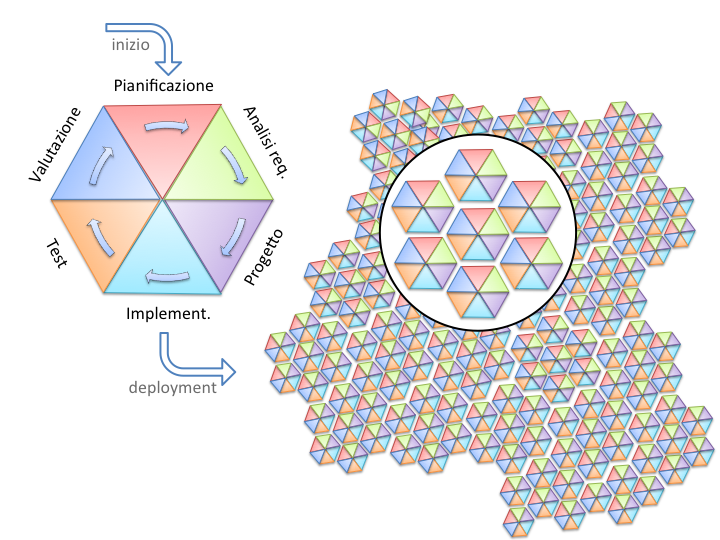
\includegraphics[scale=0.5]{img/modello_incrementale.png}
		\caption{Rappresentazione del modello incrementale\protect\footnotemark}
		\label{fig:modello_incrementale}
	\end{figure}

	\footnotetext{Fonte in \S\ref{rifinfo}}
	
\section{Descrizione generale}
testo

	\subsection{Intento del prodotto}
	testo
	
	\subsection{Funzioni del prodotto}
	testo

	\subsection{Caratteristiche degli utenti}
	testo
	
	\subsection{Vincoli del progetto}
		testo
	
		\subsubsection{Requisiti minimi}
		testo
	
		\subsubsection{Requisiti desiderabili}
		testo
\clearpage
\section{Casi d'uso}\label{CasiDUso}
Questa sezione elenca le funzionalità offerte da \progetto\ descritte attraverso il linguaggio \gloss{UML}.
\progetto\ può essere visto come l'insieme di più sottosistemi che verranno in seguito elencati e che sono stati descritti in modo molto generale anche attraverso la Figura \ref{fig:butterfly}.\par
Questa mostra in maniera un po' più chiarificante la suddivisione e ne facilita l'analisi per la stesura dei casi d'uso.
Abbiamo quindi come attori non soltanto le applicazioni che mandano messaggi al sistema, ma anche componenti quali i vari Producer e Consumer che interagiscono col Gestore Personale. \par
All'interno dei casi d'uso il termine ``sistema'' è inteso come l'intera applicazione \progetto, mentre ``piattaforma di messaggistica'' fa sempre riferimento a Telegram o Email, il termine ``persona di fiducia'' indica la persona a cui inoltrare le proprie notifiche nei giorni in cui non si è disponibili e con ``indisponibilità'' e ``irreperibilità'' di una persona si intendono proprio quei giorni in cui una persona non è raggiungibile nè disponibile per proseguire con le proprie mansioni e quindi non vuole ricevere notifiche. \par
Il termine ``identificativo'' fa riferimento indifferentemente al contatto Email o all'ID Telegram.
	
	\subsection{Attori}
	\begin{itemize}
		\item Redmine
		\item GitLab
		\item Producer Redmine
		\item Producer GitLab
		\item Utente non acceduto
		\item Utente non registrato
		\item Utente (inteso come acceduto e registrato nel sistema)
		\item Consumer Telegram
		\item Consumer Email
		\item Telegram
		\item Email
	\end{itemize}

	\subsection{Sistemi e sottosistemi}
	Per indicare i vari sottosistemi nei codici dei casi d'uso sono allegati delle sigle per rendere più chiara la posizione del caso d'uso all'interno di \progetto.
	\begin{itemize}
		%\item \textbf{B}: \progetto.
		\item \textbf{PR}: Producer Redmine.
		\item \textbf{PG}: Producer GitLab.
		\item \textbf{GP}: Gestore Personale.
		\item \textbf{CT}: Consumer telegram.
		\item \textbf{CE}: Consumer Email.
		\item \textbf{BT}: bot Telegram.
		\item \textbf{SE}: server Email.
	\end{itemize}

	\clearpage

	\subsection{Elenco casi d'uso}

%TODO: da ricordarsi: se qualcuno è offline, c'è la possibilità che il messaggio venga perso.

\newcounter{uccount}
\newcounter{subuccount}[uccount]
\newcounter{subsubuccount}[subuccount]
\newcounter{subsubsubuccount}[subsubuccount]

%\stepcounter{uccount}
%
%\subsubsection{UC\theuccount-PR - Redmine invia segnalazione al Producer Redmine}
%    \begin{figure}[H]
%		\centering
%		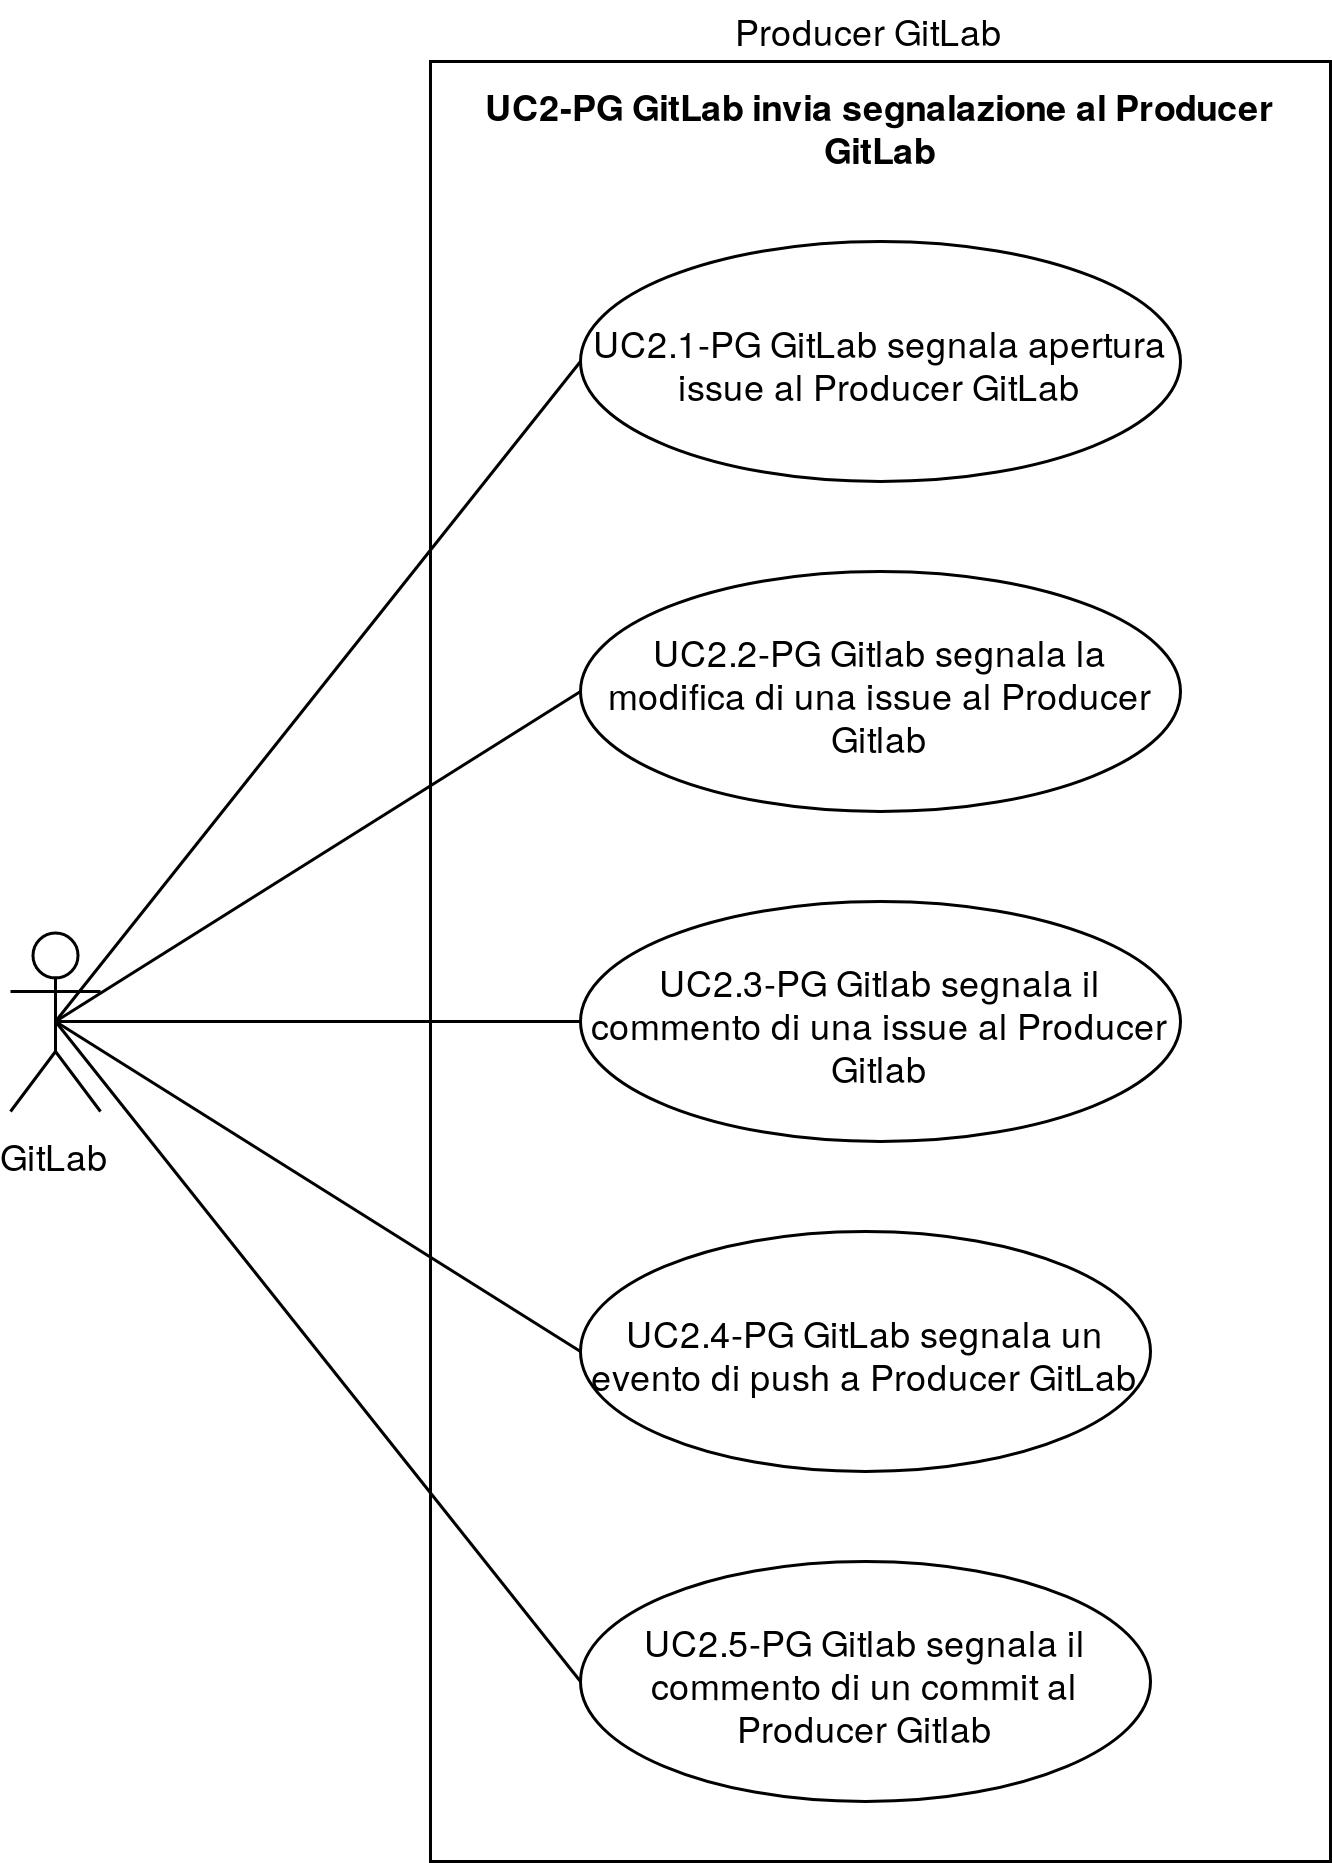
\includegraphics[width=0.5\textwidth]{img/casi_d'uso/UC2.png}\\
%		\caption{UC\theuccount-PR - Redmine segnala apertura issue al Producer Redmine}
%	\end{figure}
\begin{itemize}
	\item \textbf{Codice}: UC\theuccount-PR.
	\item \textbf{Titolo}: Redmine invia segnalazione al Producer Redmine.
	\item \textbf{Attori primari}: Redmine.
	\item \textbf{Descrizione}: Redmine invia a \progetto\ una segnalazione.
	\item \textbf{Precondizione}: su Redmine viene eseguita una operazione che scaturisce una
	segnalazione da inviare a \progetto.
	\item \textbf{Postcondizione}: il Producer Redmine riceve la segnalazione da Redmine.
	\item \textbf{Scenario principale}: 
	\begin{enumerate}
		\item Viene eseguita un'operazione
		\item Redmine procede all'invio della segnalazione al Producer Redmine
	\end{enumerate}
	
\end{itemize}

\stepcounter{subuccount}

\subsubsection{UC\theuccount.\thesubuccount-PR - Redmine segnala apertura issue al Producer Redmine}
%    \begin{figure}[H]
%		\centering
%		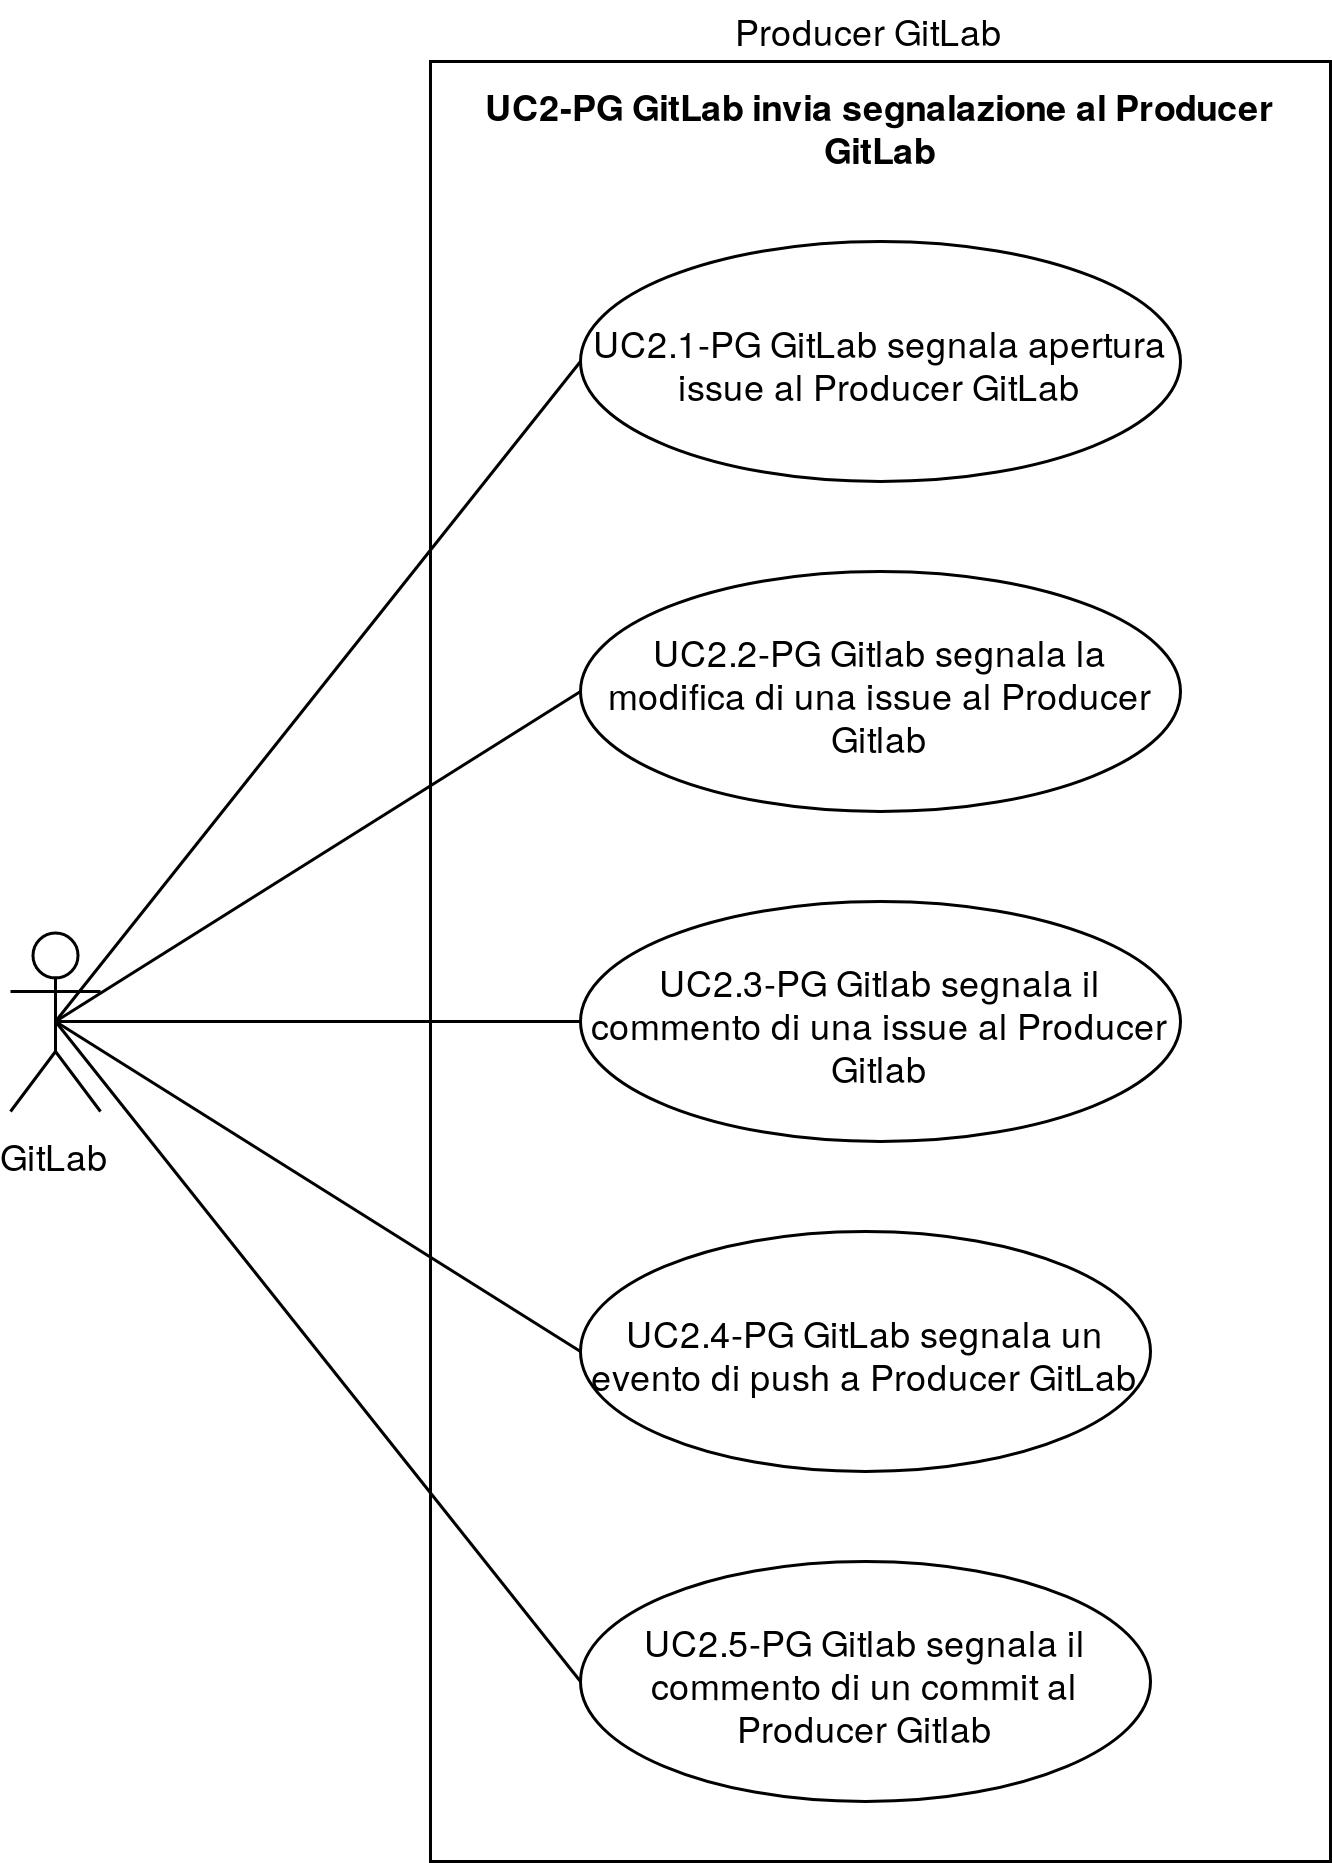
\includegraphics[width=0.5\textwidth]{img/casi_d'uso/UC2.png}\\
%		\caption{UC\theuccount-PR - Redmine segnala apertura issue al Producer Redmine}
%	\end{figure}
\begin{itemize}
	\item \textbf{Codice}: UC\theuccount-PR.
	\item \textbf{Titolo}: Redmine segnala apertura issue al Producer Redmine.
	\item \textbf{Attori primari}: Redmine.
	\item \textbf{Descrizione}: Redmine segnala a \progetto\ l'apertura di una nuova issue tramite webhook.
	
	L'apertura di una issue in un particolare progetto su Redmine contiene i seguenti campi di interesse:
	\begin{itemize}
		\item Status
		\item Tracker
		\item Subject
		\item Priority e opzionalmente:
		\begin{itemize}
			\item Description
			\item Assignee
		\end{itemize}
	\end{itemize}
	Il campo status conterrà sempre al suo interno ``opened''.
	\item \textbf{Precondizione}: Viene aperta una issue su Redmine da
	segnalare a \progetto.
	\item \textbf{Postcondizione}: il Producer Redmine riceve la segnalazione da Redmine.
	\item \textbf{Scenario principale}: 
	\begin{enumerate}
		\item Viene aperta una nuova issue su Redmine
		\item Redmine procede all'invio della segnalazione di issue al Producer Redmine
	\end{enumerate}
	
\end{itemize}

\stepcounter{subuccount}

\subsubsection{UC\theuccount.\thesubuccount-PR - Redmine segnala la modifica di una issue al Producer Redmine}
%	\begin{figure}[H]
%		\centering
%		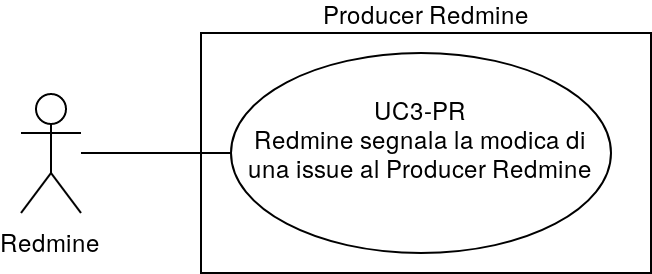
\includegraphics[width=0.5\textwidth]{img/casi_d'uso/UC3.png}\\
%		\caption{UC\theuccount-PR - Redmine segnala la modifica di una issue al Producer Redmine}
%	\end{figure}
\begin{itemize}
	\item \textbf{Codice}: UC\theuccount-PR.
	\item \textbf{Titolo}: Redmine segnala la modifica di una issue al Producer Redmine.
	\item \textbf{Attori primari}: Redmine.
	\item \textbf{Descrizione}: quando una issue viene modificata, l'invio di tale segnalazione
	avviene da parte di Redmine tramite webhook.
	I campi di interesse sono gli stessi dell'apertura di una issue, con la differenza che necessariamente il campo status contiene ora ``updated''.
	\item \textbf{Precondizione}: Viene modificata una issue già aperta su un
	progetto di Redmine da segnalare a \progetto.
	\item \textbf{Postcondizione}: il Producer Redmine riceve la segnalazione da Redmine.
	\item \textbf{Scenario principale}: 
	\begin{enumerate}
		\item Viene modificata una issue già esistente su Redmine
		\item Redmine procede all'invio della segnalazione di modifica issue al Producer Redmine
	\end{enumerate}
	
\end{itemize}

\stepcounter{subuccount}

\subsubsection{UC\theuccount.\thesubuccount-PR - Redmine segnala il commento di una issue al Producer Redmine}
%	\begin{figure}[H]
%		\centering
%		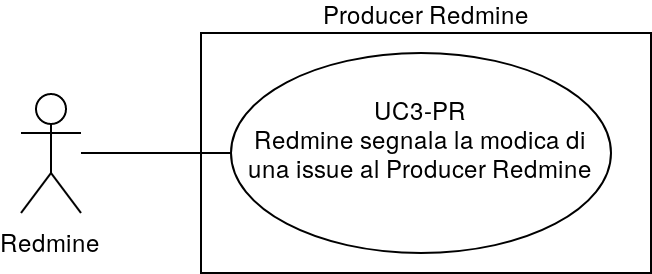
\includegraphics[width=0.5\textwidth]{img/casi_d'uso/UC3.png}\\
%		\caption{UC\theuccount-PR - Redmine segnala la modifica di una issue al Producer Redmine}
%	\end{figure}
\begin{itemize}
	\item \textbf{Codice}: UC\theuccount.\thesubuccount-PR.
	\item \textbf{Titolo}: Redmine segnala il commento di una issue al Producer Redmine.
	\item \textbf{Attori primari}: Redmine.
	\item \textbf{Descrizione}: quando una issue viene commentata, l'invio di tale segnalazione
	avviene da parte di Redmine tramite webhook.
	I campi di interesse sono gli stessi della modifica di una issue, con la differenza che necessariamente il campo status contiene ora ``updated''.
	\item \textbf{Precondizione}: Viene modificata una issue già aperta su un
	progetto di Redmine da segnalare a \progetto.
	\item \textbf{Postcondizione}: il Producer Redmine riceve la segnalazione da Redmine.
	\item \textbf{Scenario principale}: 
	\begin{enumerate}
		\item Viene modificata una issue già esistente su Redmine
		\item Redmine procede all'invio della segnalazione di modifica issue al Producer Redmine
	\end{enumerate}
	
\end{itemize}


\stepcounter{uccount}
%\clearpage
\subsubsection{UC\theuccount-PG - GitLab invia segnalazione al Producer GitLab}
	\begin{figure}[H]
		\centering
		\includegraphics[width=0.8\textwidth]{img/casi_d'uso/UC\theuccount.png}\\
		\caption{UC2-PG - GitLab invia segnalazione al Producer GitLab}
	\end{figure}
\begin{itemize}
    \item \textbf{Codice}: UC\theuccount-PG.
    \item \textbf{Titolo}: GitLab invia segnalazione al Producer GitLab.
    \item \textbf{Attori primari}: GitLab.
    \item \textbf{Descrizione}: GitLab invia una segnalazione tramite webhook a \progetto.
    \item \textbf{Precondizione}: su GitLab viene eseguita una operazione che scaturisce una
    segnalazione da inviare a \progetto.
    \item \textbf{Postcondizione}: il Producer GitLab riceve la segnalazione da GitLab.
    \item \textbf{Scenario principale}:
    \begin{enumerate}
        \item Viene eseguita un'operazione
        \item GitLab procede all'invio della segnalazione al Producer GitLab
        \item Il Producer GitLab riceve la segnalazione
    \end{enumerate}

\end{itemize}

\stepcounter{subuccount}

\subsubsection{UC\theuccount.\thesubuccount-PG - GitLab segnala apertura issue al Producer GitLab}
\begin{itemize}
    \item \textbf{Codice}: UC\theuccount.\thesubuccount-PG.
    \item \textbf{Titolo}: GitLab segnala apertura issue al Producer GitLab.
    \item \textbf{Attori primari}: GitLab.
    \item \textbf{Descrizione}: GitLab segnala l'apertura di una nuova issue tramite webhook a \progetto.
    L'apertura di una issue su GitLab contiene:
    \begin{itemize}
        \item Object kind
        \item Action
        \item Project
        \item Title e opzionalmente:
        \begin{itemize}
            \item Label
            \item Milestone
            \item Assignees
            \item Due Date
        \end{itemize}
    \end{itemize}
    Il campo object kind ci permette di capire il tipo di oggetto. In questo caso infatti contiene ``issue'', mentre il campo action ha ``open''.
    \item \textbf{Precondizione}: su GitLab viene eseguita una operazione che scaturisce una
    segnalazione da inviare a \progetto.
    \item \textbf{Postcondizione}: il Producer GitLab riceve la segnalazione di apertura issue da GitLab.
    \item \textbf{Scenario principale}:
    \begin{enumerate}
        \item Viene aperta una nuova issue su GitLab
        \item GitLab procede all'invio della segnalazione di issue al Producer GitLab
        \item Il Producer GitLab riceve la segnalazione di apertura issue
    \end{enumerate}

\end{itemize}

\stepcounter{subuccount}

\subsubsection{UC\theuccount.\thesubuccount-PG - Gitlab segnala la modifica di una issue al Producer Gitlab}
\begin{itemize}
    \item \textbf{Codice}: UC\theuccount.\thesubuccount-PG.
    \item \textbf{Titolo}: Gitlab segnala la modifica di una issue al Producer Gitlab.
    \item \textbf{Attori primari}: GitLab.
    \item \textbf{Descrizione}: GitLab segnala la modifica di una issue esistente tramite webhook a
    \newline \progetto.
    I campi di interesse sono gli stessi dell'apertura issue, con la differenza che il campo action contiene ``udpate''.
    \item \textbf{Precondizione}: su GitLab viene eseguita una operazione che scaturisce una
    segnalazione da inviare a \progetto.
    \item \textbf{Postcondizione}: il Producer GitLab riceve la segnalazione di modifica issue da GitLab.
    \item \textbf{Scenario principale}:
    \begin{enumerate}
        \item Viene modificata una issue già esistente su GitLab
        \item GitLab procede all'invio della segnalazione di modifica issue al Producer GitLab
        \item Il Producer GitLab riceve la segnalazione di modifica issue
    \end{enumerate}

\end{itemize}

\stepcounter{subuccount}

\subsubsection{UC\theuccount.\thesubuccount-PG - Gitlab segnala il commento di una issue al Producer Gitlab}
\begin{itemize}
    \item \textbf{Codice}: UC\theuccount.\thesubuccount-PG.
    \item \textbf{Titolo}: Gitlab segnala il commento di una issue al Producer Gitlab.
    \item \textbf{Attori primari}: GitLab.
    \item \textbf{Descrizione}: GitLab segnala il commento di una issue esistente tramite webhook a \progetto.
    I campi di interesse sono gli stessi dell'apertura issue, con la differenza che il campo action contiene ``issue-note''.
    \item \textbf{Precondizione}: su GitLab viene eseguita una operazione che scaturisce una
    segnalazione da inviare a \progetto.
    \item \textbf{Postcondizione}: il Producer GitLab riceve la segnalazione di commento issue da GitLab.
    \item \textbf{Scenario principale}:
    \begin{enumerate}
        \item Viene commentata una issue già esistente su GitLab
        \item GitLab procede all'invio della segnalazione di commento issue al Producer GitLab
        \item \item Il Producer GitLab riceve la segnalazione di commento di una issue
    \end{enumerate}

\end{itemize}

\stepcounter{subuccount}

\subsubsection{UC\theuccount.\thesubuccount-PG - GitLab segnala un evento di push a Producer GitLab}
\begin{itemize}
\item \textbf{Codice}: UC\theuccount.\thesubuccount-PG.
\item \textbf{Titolo}: GitLab segnala un evento di push a Producer GitLab.
\item \textbf{Attori primari}: GitLab.
\item \textbf{Descrizione}: GitLab segnala un evento di push tramite webhook a \progetto. L'evento di push può essere composto da uno o più commit.
I campi di interesse sono:
\begin{itemize}
    \item Object kind
    \item Project
    \item Repository
    \item Commits
\end{itemize}
E in questo caso il campo object kind contiene ``push''.
\item \textbf{Precondizione}: su GitLab viene eseguita una operazione che scaturisce una
segnalazione da inviare a \progetto.
\item \textbf{Postcondizione}: il Producer GitLab riceve la segnalazione di push da GitLab.
\item \textbf{Scenario principale}:
\begin{enumerate}
    \item Viene effettuato un push in GitLab
    \item GitLab procede all'invio della segnalazione di push al Producer GitLab
    \item Il Producer GitLab riceve la segnalazione dell'evento di push
\end{enumerate}

\end{itemize}

\stepcounter{subuccount}

\subsubsection{UC\theuccount.\thesubuccount-PG - Gitlab segnala il commento di un commit al Producer Gitlab}
\begin{itemize}
    \item \textbf{Codice}: UC\theuccount.\thesubuccount-PG.
    \item \textbf{Titolo}: Gitlab segnala il commento di un commit al Producer Gitlab.
    \item \textbf{Attori primari}: GitLab.
    \item \textbf{Descrizione}: GitLab segnala il commento di un commit esistente tramite webhook a \progetto.
    I campi di interesse sono gli stessi dell'apertura issue, con la differenza che il campo action contiene ``commit-note''.
    \item \textbf{Precondizione}: su GitLab viene eseguita una operazione che scaturisce una
    segnalazione da inviare a \progetto.
    \item \textbf{Postcondizione}: il Producer GitLab riceve la segnalazione di commento di commit da GitLab.
    \item \textbf{Scenario principale}:
    \begin{enumerate}
        \item Viene commentato un commit già esistente su GitLab
        \item GitLab procede all'invio della segnalazione di commento commit al Producer GitLab
        \item Il Producer GitLab riceve la segnalazione di commento di un commit
    \end{enumerate}

\end{itemize}


\stepcounter{uccount}
%\clearpage
	\subsubsection{UC\theuccount-PR - Redmine segnala la modifica di una issue al Producer Redmine}
	\begin{figure}[H]
		\centering
		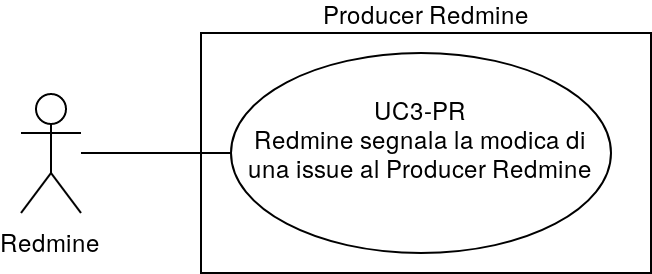
\includegraphics[width=0.7\textwidth]{img/casi_d'uso/UC3.png}\\
		\caption{UC\theuccount-PR - Redmine segnala la modifica di una issue al Producer Redmine}
	\end{figure}
	\begin{itemize}
		\item \textbf{Codice}: UC\theuccount-PR.
		\item \textbf{Titolo}: Redmine segnala la modifica di una issue al Producer Redmine.
		\item \textbf{Attori primari}: Redmine.
		\item \textbf{Descrizione}: quando una issue viene modificata, l'invio di tale segnalazione avviene da parte di Redmine tramite webhook, .
		\item \textbf{Precondizione}: Viene modificata una issue già aperta su un
		progetto di Redmine da segnalare a \progetto.
		\item \textbf{Postcondizione}: il Producer Redmine riceve la segnalazione da Redmine.
		\item \textbf{Scenario principale}: 
		\begin{enumerate}
			\item Viene modificata una issue già esistente su Redmine
			\item Redmine procede all'invio della segnalazione di modifica issue al Producer Redmine
		\end{enumerate}
		
	\end{itemize}

\stepcounter{uccount}
%\clearpage
\subsubsection{UC\theuccount-GP - Producer GitLab invia messaggio al Gestore Personale}
	\begin{figure}[H]
		\centering
		\includegraphics[width=0.8\textwidth]{img/casi_d'uso/UC\theuccount.png}\\
		\caption{UC\theuccount-GP - Producer GitLab invia messaggio al Gestore Personale}
	\end{figure}
	\begin{itemize}
		\item \textbf{Codice}: UC\theuccount-GP.
		\item \textbf{Titolo}: Producer GitLab invia messaggio al Gestore Personale.
		\item \textbf{Attori primari}: Producer GitLab.
		\item \textbf{Descrizione}: il Producer GitLab, dopo aver ricevuto una segnalazione da GitLab, elabora un messaggio da inviare al Gestore Personale. \\ Il messaggio elaborato conterrà i campi:
		\begin{itemize}
			\item App
			\item Object\_kind
			\item Title
			\item Project\_id
			\item Project\_name
			\item Author
			\item Assignees
			\item Action
			\item Description
			\item Labels
			\item Update
		\end{itemize}
        Se il Producer Gitlab riceve una segnalazione che non è in grado di analizzare, questa viene scartata.
		\item \textbf{Precondizione}: il Producer GitLab ha ricevuto una segnalazione da GitLab.
		\item \textbf{Postcondizione}: il Producer GitLab ha inviato al Gestore Personale il messaggio elaborato.
		\item \textbf{Scenario principale}:
		\begin{enumerate}
			\item Il Producer GitLab riceve una segnalazione da GitLab
			\item Il Producer GitLab prepara il messaggio in modo che venga inserito correttamente nel Gestore Personale
			\item Il Poducer GitLab invia il messaggio al Gestore Personale
            \item Il Gestore Perosonale riceve il messaggio dal Producer GitLab
		\end{enumerate}
	\end{itemize}

	\stepcounter{subuccount}

	\subsubsection{UC\theuccount.\thesubuccount-GP - Producer GitLab invia messaggio di push al Gestore Personale}

		\begin{itemize}
			\item \textbf{Codice}: UC\theuccount.\thesubuccount-GP.
			\item \textbf{Titolo}: Producer GitLab invia uno o più messaggi di commit al Gestore Personale.
			\item \textbf{Attori primari}: Producer GitLab.
			\item \textbf{Descrizione}: il Producer GitLab, dopo aver ricevuto una segnalazione di push da  \newline GitLab, suddivide la segnalazione per i commit in più messaggi che verranno catalogati sotto il Topic ``commits''.
			\item \textbf{Precondizione}: il Producer GitLab ha ricevuto una segnalazione da GitLab.
			\item \textbf{Postcondizione}: il Producer GitLab ha inviato uno o più messaggi di commit.
			\item \textbf{Scenario principale}:
			\begin{enumerate}
				\item Il Producer GitLab riceve la segnalazione di un push da GitLab
				\item Il Producer GitLab prepara i messaggi in modo che vengano inseriti correttamente nel Gestore Personale
				\item Il Producer GitLab invia i messaggi di
				commit al Gestore Personale
                \item Il Gestore Personale riceve i messaggi di commit
			\end{enumerate}
%			\item \textbf{Estensioni}:
%			\begin{enumerate}
%				\item Se ci sono dei messaggi non validi, questi vengono scartati [UC\theuccount.6-GP].
%			\end{enumerate}
		\end{itemize}

	\stepcounter{subuccount}

	\subsubsection{UC\theuccount.\thesubuccount-GP - Producer GitLab invia messaggio di una nuova issue al Gestore Personale}

	\begin{itemize}
		\item \textbf{Codice}: UC\theuccount.\thesubuccount-GP.
		\item \textbf{Titolo}: Producer GitLab invia messaggio di una nuova issue al Gestore Personale.
		\item \textbf{Attori primari}: Producer GitLab.
		\item \textbf{Descrizione}: il Producer GitLab, dopo aver ricevuto una segnalazione di una nuova issue da GitLab, elabora il messaggio da inoltrare al Gestore Personale.
		\item \textbf{Precondizione}: il Producer GitLab ha ricevuto una segnalazione da GitLab.
		\item \textbf{Postcondizione}: il Producer GitLab ha inviato al Gestore Personale il messaggio
		elaborato di nuova issue.
		\item \textbf{Scenario principale}:
		\begin{enumerate}
			\item Il Producer GitLab riceve la segnalazione di una nuova issue da GitLab
			\item Il Producer GitLab prepara il messaggio di una nuova issue in modo che venga inserito correttamente
			nel Gestore Personale
			\item Il Producer GitLab invia il messaggio di una nuova issue al Gestore Personale
			\item Il Gestore Personale riceve il messaggio di apertura issue dal Producer GitLab
		\end{enumerate}
%		\item \textbf{Estensioni}:
%		\begin{enumerate}
%			\item Se ci sono dei messaggi non validi, questi vengono scartati [UC\theuccount.6-GP].
%		\end{enumerate}
	\end{itemize}

	\stepcounter{subuccount}

	\subsubsection{UC\theuccount.\thesubuccount-GP - Producer GitLab invia messaggio di modifica di una issue al Gestore Personale}
		\begin{itemize}
			\item \textbf{Codice}: UC\theuccount.\thesubuccount-GP.
			\item \textbf{Titolo}: Producer GitLab invia messaggio di modifica di una issue al Gestore Personale.
			\item \textbf{Attori primari}: Producer GitLab.
			\item \textbf{Descrizione}: il Producer GitLab, dopo aver ricevuto una segnalazione di una modifica issue da GitLab, elabora il messaggio da inoltrare al Gestore Personale.
			% Il messaggio, una volta elaborato, conterrà i campi:
			% \begin{itemize}
			% 	\item Project
            %     \item Author
			% 	\item Topic
			% 	\item Subject e opzionalmente:
			% 	\begin{itemize}
			% 		\item Description
			% 		\item Due Date
			% 		\item Milestone
			% 		\item Assignee
			% 	\end{itemize}
			% \end{itemize}
			\item \textbf{Precondizione}: il Producer GitLab ha ricevuto una segnalazione da GitLab.
			\item \textbf{Postcondizione}: il Producer GitLab ha inviato al Gestore Personale il messaggio
			elaborato di modifica issue.
			\item \textbf{Scenario principale}:
			\begin{enumerate}
				\item Il Producer GitLab riceve la segnalazione di issue da GitLab
				\item Il Producer GitLab prepara il messaggio di modifica issue in modo che venga inserito correttamente nel Gestore Personale
				\item Il Producer GitLab invia il messaggio di issue al Gestore Personale
                \item Il Gestore Personale riceve il messaggio di modifica issue dal Producer GitLab
			\end{enumerate}
%			\item \textbf{Estensioni}:
%			\begin{enumerate}
%				\item Se ci sono dei messaggi non validi, questi vengono scartati [UC\theuccount.6-GP].
%			\end{enumerate}
		\end{itemize}

		\stepcounter{subuccount}

		\subsubsection{UC\theuccount.\thesubuccount-GP - Producer GitLab invia messaggio di commento di una issue al Gestore Personale}
		\begin{itemize}
			\item \textbf{Codice}: UC\theuccount.\thesubuccount-GP.
			\item \textbf{Titolo}: Producer GitLab invia messaggio di commento di una issue al Gestore Personale.
			\item \textbf{Attori primari}: Producer GitLab.
			\item \textbf{Descrizione}: il Producer GitLab, dopo aver ricevuto una segnalazione di commento di una issue da GitLab, elabora il messaggio da inoltrare al Gestore Personale.
			\item \textbf{Precondizione}: il Producer GitLab ha ricevuto una segnalazione da GitLab.
			\item \textbf{Postcondizione}: il Producer GitLab ha inviato al Gestore Personale il messaggio
			elaborato di commento issue.
			\item \textbf{Scenario principale}:
			\begin{enumerate}
				\item Il Producer GitLab riceve la segnalazione di commento issue da GitLab
				\item Il Producer GitLab prepara il messaggio di commento issue in modo che venga inserito correttamente nel Gestore Personale
				\item Il Producer GitLab invia il messaggio di commento issue al Gestore Personale
				\item Il Gestore Personale riceve il messaggio di commento issue dal Producer GitLab
			\end{enumerate}
%			\item \textbf{Estensioni}:
%			\begin{enumerate}
%				\item Se ci sono dei messaggi non validi, questi vengono scartati [UC\theuccount.6-GP].
%			\end{enumerate}
		\end{itemize}

		\stepcounter{subuccount}

		\subsubsection{UC\theuccount.\thesubuccount-GP - Producer GitLab invia messaggio di commento di un commit al Gestore Personale}
		\begin{itemize}
			\item \textbf{Codice}: UC\theuccount.\thesubuccount-GP.
			\item \textbf{Titolo}: Producer GitLab invia messaggio di commento di un commit al Gestore Personale.
			\item \textbf{Attori primari}: Producer GitLab.
			\item \textbf{Descrizione}: il Producer GitLab, dopo aver ricevuto una segnalazione di commento di un commit da GitLab, elabora il messaggio da inoltrare al Gestore Personale.
			\item \textbf{Precondizione}: il Producer GitLab ha ricevuto una segnalazione da GitLab.
			\item \textbf{Postcondizione}: il Producer GitLab ha inviato al Gestore Personale il messaggio
			elaborato di commento commit.
			\item \textbf{Scenario principale}:
			\begin{enumerate}
				\item Il Producer GitLab riceve la segnalazione di commento commit da GitLab
				\item Il Producer GitLab prepara il messaggio di commento commit in modo che venga inserito correttamente nel Gestore Personale
				\item Il Producer GitLab invia il messaggio di commento commit al Gestore Personale
				\item Il Gestore Personale riceve il messaggio di commento issue dal Producer GitLab
			\end{enumerate}
%			\item \textbf{Estensioni}:
%			\begin{enumerate}
%				\item Se ci sono dei messaggi non validi, questi vengono scartati [UC\theuccount.6-GP].
%			\end{enumerate}
		\end{itemize}


\stepcounter{uccount}
%\clearpage
\subsubsection{UC\theuccount-CT - Gestore Personale invia il messaggio finale al Consumer Telegram}
%	\begin{figure}[H]
%		\centering
%		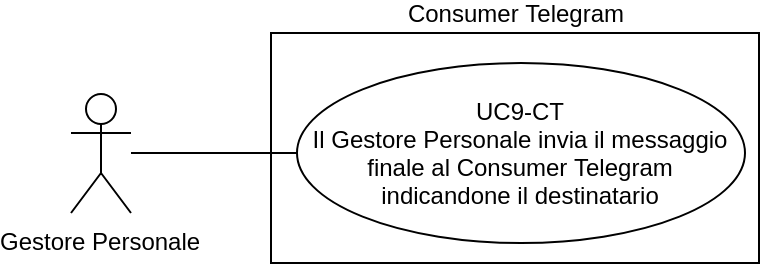
\includegraphics[width=0.6\textwidth]{img/casi_d'uso/UC9.png}\\
%		\caption{UC\theuccount-CT - Gestore Personale invia il messaggio finale al Consumer Telegram}
%	\end{figure}
	\begin{itemize}
		\item \textbf{Codice}: UC\theuccount-CT.
		\item \textbf{Titolo}: Gestore Personale invia il messaggio finale al Consumer Telegram.
		\item \textbf{Attori primari}: Gestore Personale.
		\item \textbf{Descrizione}: il Gestore Personale, dopo aver ricevuto il messaggio elaborato
		dal Producer Redmine o GitLab, controlla i Topic del messaggio, gli utenti iscritti, la loro disponibilità e se la loro preferenza è Telegram.
		Se tutte queste condizioni sono verificate, viene preparato il messaggio finale da inviare successivamente viene inviato al Consumer Telegram. 
		Se il destinatario è iscritto a quel Topic ma non è disponibile, il destinatario viene cambiato con la persona di fiducia. \par
		Il messaggio finale, una volta elaborato, conterrà i campi:
		\begin{itemize}
			\item Id della chat del destinatario
			\item Applicazione di provenienza
			\item Ora di invio
			\item Tipo di segnalazione(commit o issue)
			\item Project
			\item Topic
			\item Subject e opzionalmente
		 	\begin{itemize}
				\item Description
				\item Due date
				\item Milestone
				\item Assignee
			\end{itemize}
		\end{itemize}
		\item \textbf{Precondizione}: il Gestore Personale ha ricevuto il messaggio elaborato dal Producer Redmine o GitLab.
		\item \textbf{Postcondizione}: Il Gestore Personale ha inviato il messaggio finale al Consumer Telegram.
		\item \textbf{Scenario principale}: 
		\begin{enumerate}
			\item ll Gestore Personale riceve un messaggio dal Producer Redmine o dal Producer GitLab
			\item Il Gestore Personale valuta quali utenti sono iscritti al Topic del messaggio ricevuto e se vogliono ricevere il messaggio tramite Telegram
			\item Il Gestore Personale procede all'invio del messaggio finale al Consumer Telegram
		\end{enumerate}
		
	\end{itemize}

\stepcounter{uccount}
%\clearpage
\subsubsection{UC\theuccount-PG - GitLab segnala un evento di push a Producer GitLab}
%	\begin{figure}[H]
%		\centering
%		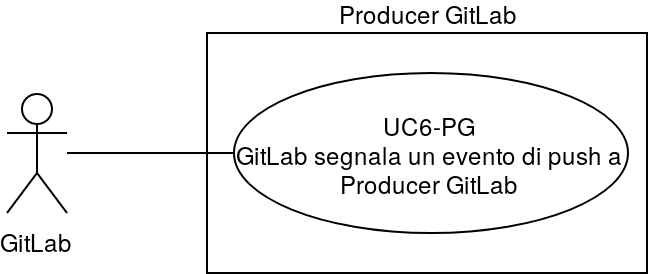
\includegraphics[width=0.5\textwidth]{img/casi_d'uso/UC6.png}\\
%		\caption{UC\theuccount-PG - GitLab segnala un evento di push a Producer GitLab}
%	\end{figure}
	\begin{itemize}
		\item \textbf{Codice}: UC\theuccount-PG.
		\item \textbf{Titolo}: GitLab segnala un evento di push a Producer GitLab.
		\item \textbf{Attori primari}: GitLab.
		\item \textbf{Descrizione}: GitLab segnala un evento di push tramite webhook a \progetto. L'evento di	push può essere composto da uno o più commit.
		I campi di interesse sono:
		\begin{itemize}
			\item Object kind
			\item Project
			\item Repository
			\item Commits
		\end{itemize}
		E in questo caso il campo object kind contiene ``push''.
		\item \textbf{Precondizione}: Viene effettuato un push su GitLab da segnalare a \progetto.
		\item \textbf{Postcondizione}: il Producer GitLab riceve la segnalazione da GitLab.
		\item \textbf{Scenario principale}: 
		\begin{enumerate}
			\item Viene effettuato un push in GitLab
			\item GitLab procede all'invio della segnalazione di push al Producer GitLab
		\end{enumerate}
		
	\end{itemize}

\stepcounter{uccount}
%\clearpage
\subsubsection{UC\theuccount-GP - Producer Redmine invia messaggio al Gestore Personale}
    \begin{figure}[H]
		\centering
		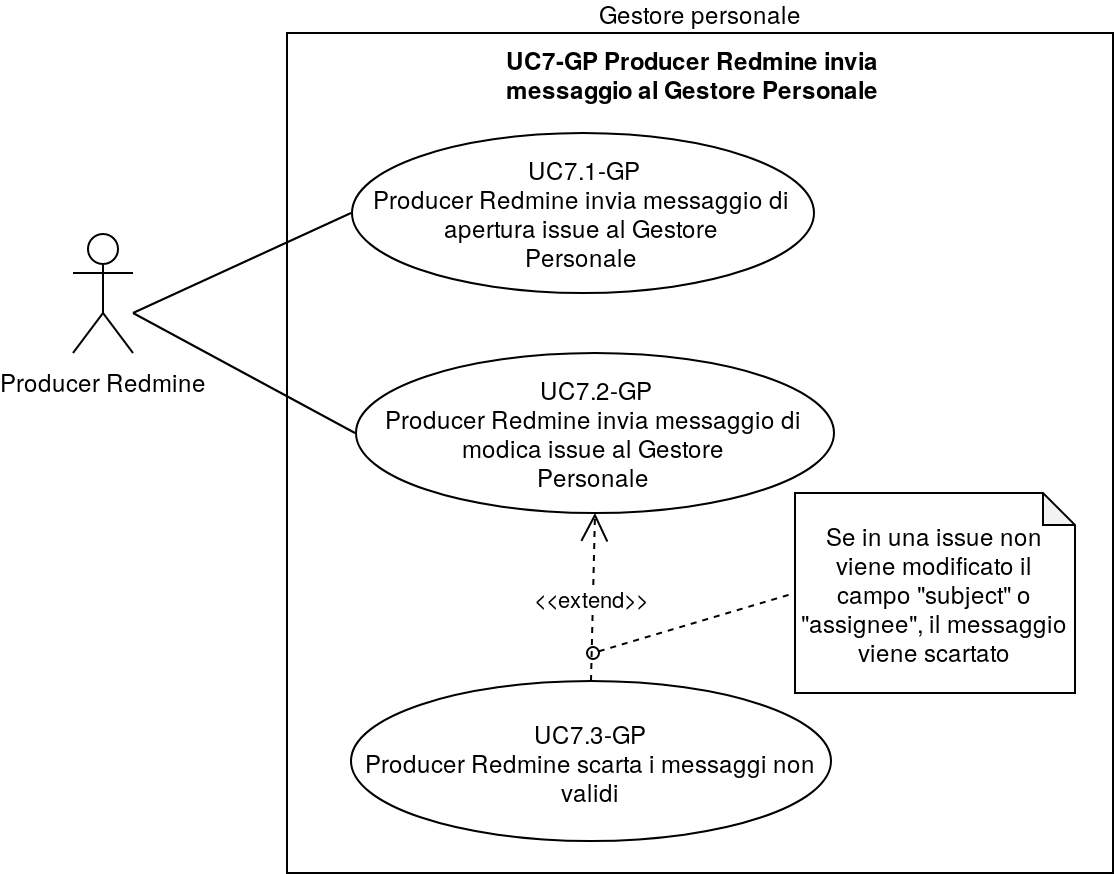
\includegraphics[width=0.8\textwidth]{img/casi_d'uso/UC7.png}\\
		\caption{UC\theuccount-GP - Producer Redmine invia messaggio al Gestore Personale}
	\end{figure}
	\begin{itemize}
		\item \textbf{Codice}: UC\theuccount-GP.
		\item \textbf{Titolo}: Producer Redmine invia messaggio al Gestore Personale.
		\item \textbf{Attori Pimari}: Producer Redmine.
		\item \textbf{Descrizione}: il Producer Redmine, dopo aver ricevuto una
		 segnalazione da Redmine, elabora il messaggio e lo invia al Gestore Personale.
		 Il messaggio finale, una volta terminata l'elaborazione, conterrà i campi:
		 \begin{itemize}
		 	\item Poject
		 	\item Topic
		 	\item Subject e opzionalmente:
		 	\begin{itemize}
		 		\item Description
		 	\end{itemize}
		 \end{itemize}
	 	Il messaggio non può contenere campi errati o mancanti per il corretto funzionamenti di \progetto, perché i campi selezionati sono obbligatori per l'apertura di una issue su Redmine.
		\item \textbf{Pecondizione}: il Producer Redmine ha ricevuto una segnalazione da Redmine.
		\item \textbf{Postcondizione}: il Producer Redmine ha elaborato e inviato al Gestore Personale il messaggio.
		\item \textbf{Scenario GPincipale}: 
		\begin{enumerate}
			\item Il Producer Redmine riceve la segnalazione di issue da Redmine
			\item Il Producer Redmine prepara il messaggio di issue in modo che venga inserito correttamente nel Gestore Personale
			\item Il Producer Redmine invia il messaggio di issue al Gestore Personale
		\end{enumerate}
		
	\end{itemize}
	
	\stepcounter{subuccount}
	\paragraph{UC\theuccount.\thesubuccount-GP - Producer Redmine invia messaggio di apertura issue al Gestore Personale}
	
	\begin{itemize}
		\item \textbf{Codice}: UC\theuccount.\thesubuccount-GP.
		\item \textbf{Titolo}: Producer Redmine invia messaggio di apertura issue al Gestore Personale.
		\item \textbf{Attori Pimari}: Producer Redmine.
		\item \textbf{Descrizione}: il Producer Redmine, dopo aver
		ricevuto una segnalazione di apertura issue da Redmine, elabora il messaggio e lo invia al Gestore Personale.
		Il messaggio finale, una volta terminata l'elaborazione, conterrà i campi:
		\begin{itemize}
			\item Poject
			\item Topic
			\item Subject e opzionalmente:
			\begin{itemize}
				\item Description
			\end{itemize}
		\end{itemize}
		\item \textbf{Pecondizione}: il Producer Redmine ha ricevuto una segnalazione da Redmine.
		\item \textbf{Postcondizione}: il GPoducer Redmine ha elaborato e inviato al Gestore Personale il messaggio di apertura issue.
		\item \textbf{Scenario Pincipale}: 
		\begin{enumerate}
			\item Il Producer Redmine riceve la segnalazione di apertura issue da Redmine
			\item Il Producer Redmine prepara il messaggio in modo che venga inserito correttamente nel Gestore Personale
			\item Il Producer Redmine invia il messaggio di
			apertura issue al Gestore Personale
		\end{enumerate}
		
	\end{itemize}
	
	\stepcounter{subuccount}
	\paragraph{UC\theuccount.\thesubuccount-GP - Producer Redmine invia messaggio di modifica issue al Gestore Personale}
		
		\begin{itemize}
			\item \textbf{Codice}: UC\theuccount.\thesubuccount-GP.
			\item \textbf{Titolo}: Producer Redmine invia messaggio di modifica issue al Gestore Personale
			\item \textbf{Attori Pimari}: Producer Redmine.
			\item \textbf{Descrizione}: il Producer Redmine, dopo aver
			ricevuto una segnalazione di modifica issue da Redmine, elabora il messaggio e lo invia al Gestore Personale.
			Il messaggio finale, una volta terminata l'elaborazione, conterrà i campi:
			\begin{itemize}
				\item Poject
				\item Topic
				\item Subject e opzionalmente:
				\begin{itemize}
					\item Description
				\end{itemize}
			\end{itemize}
			\item \textbf{Pecondizione}: il Producer Redmine ha ricevuto una segnalazione da Redmine.
			\item \textbf{Postcondizione}: il Producer Redmine ha elaborato e inviato al Gestore Personale il messaggio di modifica issue.
			\item \textbf{Scenario Pincipale}: 
			\begin{enumerate}
				\item Il Producer Redmine riceve la segnalazione di modifica issue da Redmine
				\item Il Producer Redmine prepara il messaggio in modo che venga inserito correttamente nel Gestore Personale
				\item Il Producer Redmine invia il messaggio di
				modifica issue al Gestore Personale
			\end{enumerate}
			
		\end{itemize}
	
	\stepcounter{subuccount}
	\paragraph{UC\theuccount.\thesubuccount-GP - Producer Redmine scarta i messaggi non validi}
	
	\begin{itemize}
		\item \textbf{Codice}: UC\theuccount.\thesubuccount-GP.
		\item \textbf{Titolo}: Producer Redmine scarta i messaggi non validi.
		\item \textbf{Attori primari}: Producer Redmine.
		\item \textbf{Descrizione}: il Producer Redmine, dopo aver ricevuto una segnalazione di una modifica issue da Redmine, controlla
		se è stato modificato il campo Subject. In caso negativo, il messaggio viene scartato.
		\item \textbf{Precondizione}: il Producer Redmine ha ricevuto una segnalazione da GitLab.
		\item \textbf{Postcondizione}: il Producer Redmine ha scartato il messaggio.
		\item \textbf{Scenario principale}: 
		\begin{enumerate}
			\item Il Producer Redmine riceve la segnalazione di modifica issue da Redmine
			\item Il Producer Redmine vede che non è stato modificato il campo Subject
			\item Il Producer Redmine scarta il messaggio non valido.
		\end{enumerate}
	\end{itemize}

\stepcounter{uccount}
%\clearpage
\subsubsection{UC\theuccount-SE - Consumer Email inoltra il messaggio finale al server Email}
	\begin{figure}[H]
		\centering
		\includegraphics[width=0.7\textwidth]{img/casi_d'uso/UC\theuccount.png}\\
		\caption{UC\theuccount-SE - Consumer Email inoltra il messaggio finale al server Email}
	\end{figure}
	\begin{itemize}
		\item \textbf{Codice}: UC\theuccount-SE.
		\item \textbf{Titolo}: Consumer Email inoltra il messaggio finale al server Email.
		\item \textbf{Attori primari}: Consumer Email.
		\item \textbf{Descrizione}: il Consumer Email inoltra il messaggio finale al server Email, il quale notifica il destinatario finale attraverso una mail.
		\item \textbf{Precondizione}: il Consumer Email ha ricevuto almeno un messaggio.
		\item \textbf{Postcondizione}: il server Email ha ricevuto il messaggio finale.
		\item \textbf{Scenario principale}:
		\begin{enumerate}
			\item Il Consumer Email riceve un messaggio dal Gestore Personale
			\item Il Consumer Email procede all'inoltro del messaggio finale al server Email
            \item Il server Email riceve il messaggio dal Consumer Email
		\end{enumerate}

	\end{itemize}


\stepcounter{uccount}
%\clearpage
\subsubsection{UC\theuccount-CT - Gestore Personale invia il messaggio finale al Consumer Telegram}
%	\begin{figure}[H]
%		\centering
%		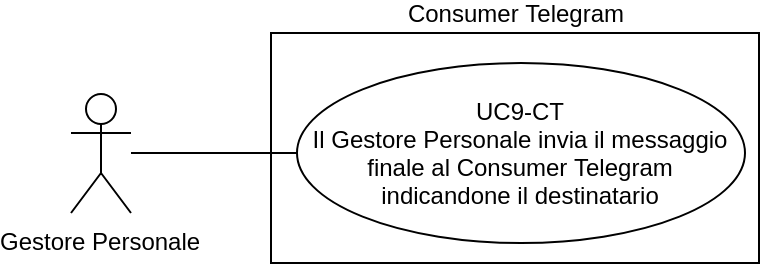
\includegraphics[width=0.6\textwidth]{img/casi_d'uso/UC9.png}\\
%		\caption{UC\theuccount-CT - Gestore Personale invia il messaggio finale al Consumer Telegram}
%	\end{figure}
	\begin{itemize}
		\item \textbf{Codice}: UC\theuccount-CT.
		\item \textbf{Titolo}: Gestore Personale invia il messaggio finale al Consumer Telegram.
		\item \textbf{Attori primari}: Gestore Personale.
		\item \textbf{Descrizione}: il Gestore Personale, dopo aver ricevuto il messaggio elaborato
		dal Producer Redmine o GitLab, controlla i Topic del messaggio, gli utenti iscritti, la loro disponibilità e se la loro preferenza è Telegram.
		Se tutte queste condizioni sono verificate, viene preparato il messaggio finale da inviare successivamente viene inviato al Consumer Telegram. 
		Se il destinatario è iscritto a quel Topic ma non è disponibile, il destinatario viene cambiato con la persona di fiducia. \par
		Il messaggio finale, una volta elaborato, conterrà i campi:
		\begin{itemize}
			\item Id della chat del destinatario
			\item Applicazione di provenienza
			\item Ora di invio
			\item Tipo di segnalazione(commit o issue)
			\item Project
			\item Topic
			\item Subject e opzionalmente
		 	\begin{itemize}
				\item Description
				\item Due date
				\item Milestone
				\item Assignee
			\end{itemize}
		\end{itemize}
		\item \textbf{Precondizione}: il Gestore Personale ha ricevuto il messaggio elaborato dal Producer Redmine o GitLab.
		\item \textbf{Postcondizione}: Il Gestore Personale ha inviato il messaggio finale al Consumer Telegram.
		\item \textbf{Scenario principale}: 
		\begin{enumerate}
			\item ll Gestore Personale riceve un messaggio dal Producer Redmine o dal Producer GitLab
			\item Il Gestore Personale valuta quali utenti sono iscritti al Topic del messaggio ricevuto e se vogliono ricevere il messaggio tramite Telegram
			\item Il Gestore Personale procede all'invio del messaggio finale al Consumer Telegram
		\end{enumerate}
		
	\end{itemize}

\stepcounter{uccount}
%\clearpage
\subsubsection{UC\theuccount-CE - Gestore Personale invia il messaggio finale al Consumer Email}
	\begin{figure}[H]
		\centering
		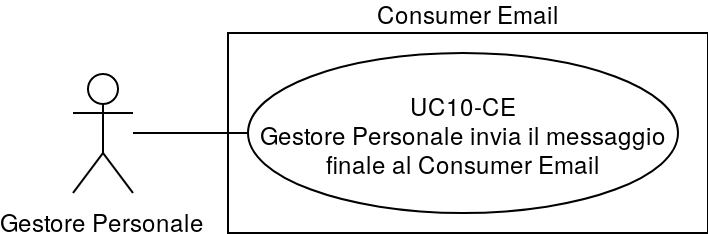
\includegraphics[width=0.6\textwidth]{img/casi_d'uso/UC10.png}\\
		\caption{UC\theuccount-CE - Gestore Personale invia il messaggio finale al Consumer Email}
	\end{figure}
	\begin{itemize}
		\item \textbf{Codice}: UC\theuccount-CE.
		\item \textbf{Titolo}: Gestore Personale invia il messaggio finale al Consumer Email.
		\item \textbf{Attori primari}: Gestore Personale.
		\item \textbf{Descrizione}: il Gestore Personale, dopo aver ricevuto il messaggio elaborato dai
		Producer Redmine o GitLab, controlla i messaggi sullo specifico Topic "commits", se ce ne sono
		vengono analizzati in base alla	lista di keyword. Se gli utenti iscritti a quella determinata
		keyword sono disponibili e se vogliono ricevere il messaggio tramite Email viene preparato il
		messaggio finale da inviare e inviato al Consumer Email. Altrimenti valuta il campo Topic del
		messaggio e controlla chi è iscritto a quel Topic, se gli utenti iscritti a quel Topic sono
		disponibili e se vogliono ricevere il messaggio tramite Email. Se tutte queste condizioni sono
		verificate, viene preparato il messaggio finale da inviare e inviato al Consumer Email.\\
		Il messaggio finale, una volta elaborato, conterrà i campi:
		\begin{itemize}
			\item Email del destinatario
			\item Applicazione di provenienza
			\item Ora di invio
			\item Tipo di segnalazione(commit, issue)
			\item Project
			\item Topic
			\item Subject e opzionalmente
		 	\begin{itemize}
				\item Description
				\item Due date
				\item Milestone
				\item Assignee
			\end{itemize}
		\end{itemize}
		\item \textbf{Precondizione}: il Gestore Personale ha ricevuto il messaggio elaborato dai Producer Redmine o GitLab.
		\item \textbf{Postcondizione}: Il Gestore Personale ha inviato il messaggio finale al Consumer Email.
		\item \textbf{Scenario principale}: 
		\begin{enumerate}
			\item ll Gestore Personale riceve un messaggio dal Producer Redmine o dal Producer GitLab
			\item Il Gestore Personale valuta quali utenti sono iscritti al Topic del messaggio ricevuto, se sono disponibili e se vogliono ricevere il messaggio tramite Email
			\item Gestore Personale procede all'invio del messaggio finale al Consumer Email
		\end{enumerate}
		
	\end{itemize}

\stepcounter{uccount}
%\clearpage
\subsubsection{UC\theuccount-GP - Inserimento utente}
		\begin{figure}[H]
			\centering
				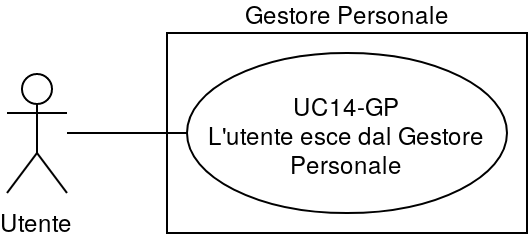
\includegraphics[width=\columnwidth]{img/casi_d'uso/UC14.png}\\
			\caption{UC\theuccount-GP - Inserimento utente}
		\end{figure}
	\begin{itemize}
		\item \textbf{Codice}: UC\theuccount-GP.
		\item \textbf{Titolo}: Inserimento utente.
		\item \textbf{Attori primari}: utente.
		\item \textbf{Descrizione}: l'utente, acceduto al sistema, aggiunge un nuovo utente nel sistema.
		Non è possibile che un utente non acceduto si iscriva da solo per la prima volta.
		In un primo momento è presente solo un utente predefinito che può aggiungere gli altri utenti.
		\item \textbf{Precondizione}: un nuovo utente deve essere aggiunto nel sistema.
		\item \textbf{Postcondizione}: un utente viene aggiunto al sistema.
		\item \textbf{Scenario principale}:
		\begin{enumerate}
			\item L'utente aggiunge un nuovo utente
		\end{enumerate}
	\end{itemize}
	%TODO:  aggiuora io, povero stronzo, che sono statonto.. come faccio a sapere qual è il mio identificativo?!
	\stepcounter{subuccount}
	\subsubsection{UC\theuccount.\thesubuccount-GP - Aggiunta nuovo utente}
		\begin{figure}[H]
			\centering
			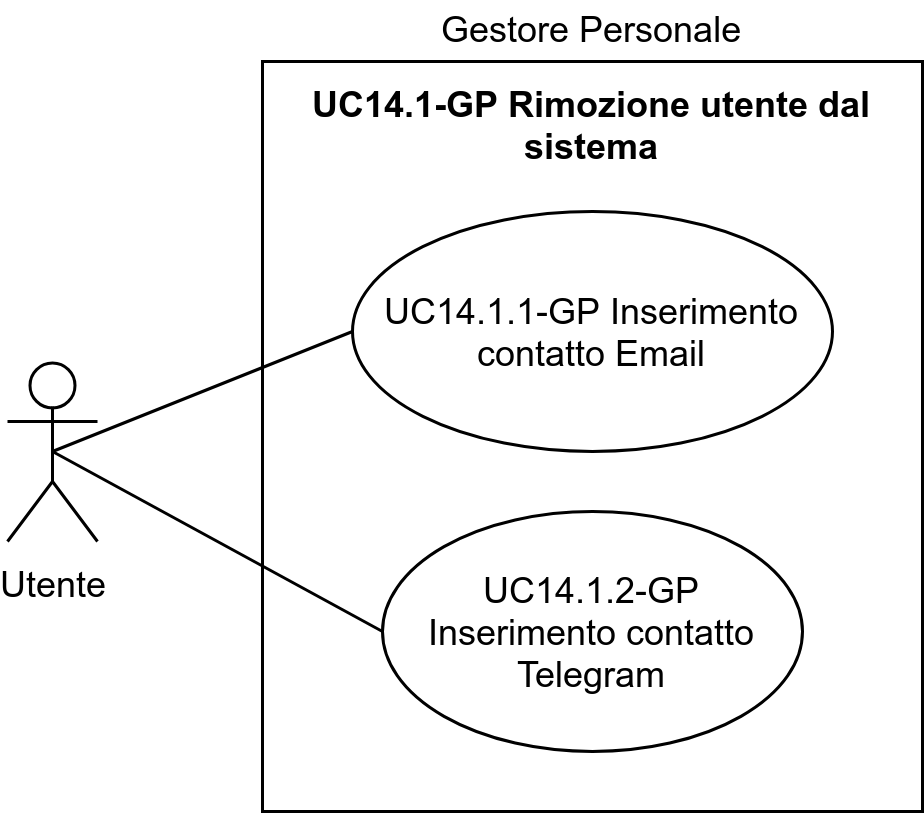
\includegraphics[width=\columnwidth]{img/casi_d'uso/UC14_1.png}\\
			\caption{UC\theuccount.\thesubuccount-GP - Aggiunta nuovo utente}
		\end{figure}
		\begin{itemize}
			\item \textbf{Codice}: C\theuccount.\thesubuccount-GP.
			\item \textbf{Titolo}: Aggiunta nuovo utente.
			\item \textbf{Attori primari}: utente.
			\item \textbf{Descrizione}: un nuovo utente viene inserito nel sistema.
			\item \textbf{Precondizione}: un nuovo utente deve essere aggiunto nel sistema.
			\item \textbf{Postcondizione}: un utente viene aggiunto al sistema.
			\item \textbf{Scenario principale}:
			\begin{enumerate}
				\item L'utente inserisce i dati del nuovo utente da aggiungere
				\item L'utente conferma l'invio dei dati
				\item L'aggiunta viene effettuata
			\end{enumerate}
			\item \textbf{Estensioni}:
			\begin{enumerate}
				\item Errore utente già presente nel sistema [UC\theuccount.2-GP]
			\end{enumerate}
		\end{itemize}

		\stepcounter{subsubuccount}
		\subsubsection{UC\theuccount.\thesubuccount.\thesubsubuccount-GP - Inserimento nome utente}

			\begin{itemize}
				\item \textbf{Codice}: UC\theuccount.\thesubuccount.\thesubsubuccount-GP.
				\item \textbf{Titolo}: inserimento nome utente.
				\item \textbf{Attori primari}: utente.
				%non registrato.
				\item \textbf{Descrizione}: l'utente inserisce il nominativo dell'utente da aggiungere.
				\item \textbf{Precondizione}: un nuovo utente deve essere aggiunto nel sistema.
				\item \textbf{Postcondizione}: il nome del nuovo utente è stato aggiunto nel sistema.
				\item \textbf{Scenario principale}:
				\begin{enumerate}
					\item L'utente aggiunge il nominativo del nuovo utente
				\end{enumerate}
			\end{itemize}

		\stepcounter{subsubuccount}
		\subsubsection{UC\theuccount.\thesubuccount.\thesubsubuccount-GP - Inserimento cognome utente}

			\begin{itemize}
				\item \textbf{Codice}: UC\theuccount.\thesubuccount.\thesubsubuccount-GP.
				\item \textbf{Titolo}: inserimento cognome utente.
				\item \textbf{Attori primari}: utente.
				% non registrato.
				\item \textbf{Descrizione}: l'utente inserisce il cognome dell'utente da aggiungere.
				\item \textbf{Precondizione}: un nuovo utente deve essere aggiunto nel sistema.
				\item \textbf{Postcondizione}: il cognome del nuovo utente è stato aggiunto nel sistema.
				\item \textbf{Scenario principale}:
				\begin{enumerate}
					\item L'utente aggiunge il cognome del nuovo utente
				\end{enumerate}
			\end{itemize}

		\stepcounter{subsubuccount}
		\subsubsection{UC\theuccount.\thesubuccount.\thesubsubuccount-GP - Inserimento contatto Email}

			\begin{itemize}
				\item \textbf{Codice}: UC\theuccount.\thesubuccount.\thesubsubuccount-GP.
				\item \textbf{Titolo}: inserimento contatto Email.
				\item \textbf{Attori primari}: utente.
				% non registrato.
				\item \textbf{Descrizione}: l'utente inserisce il contatto Email dell'utente da aggiungere.
				\item \textbf{Precondizione}: un nuovo utente deve essere aggiunto nel sistema.
				\item \textbf{Postcondizione}: il contatto Email è stato aggiunto.
				\item \textbf{Scenario principale}:
				\begin{enumerate}
					\item L'utente aggiunge il contatto Email del nuovo utente
				\end{enumerate}
		\end{itemize}

		\stepcounter{subsubuccount}
		\subsubsection{UC\theuccount.\thesubuccount.\thesubsubuccount-GP - Inserimento contatto Telegram}

			\begin{itemize}
				\item \textbf{Codice}: UC\theuccount.\thesubuccount.\thesubsubuccount-GP.
				\item \textbf{Titolo}: inserimento contatto Telegram.
				\item \textbf{Attori primari}: utente.
				% non registrato.
				\item \textbf{Descrizione}: l'utente inserisce il contatto Telegram dell'utente da aggiungere.
				\item \textbf{Precondizione}: un nuovo utente deve essere aggiunto nel sistema.
				\item \textbf{Postcondizione}: il contatto Telegram è stato aggiunto.
				\item \textbf{Scenario principale}:
				\begin{enumerate}
					\item L'utente aggiunge il contatto Telegram del nuovo utente
				\end{enumerate}
			\end{itemize}

	\stepcounter{subuccount}
	\subsubsection{UC\theuccount.\thesubuccount-GP - Errore utente già presente nel sistema}

		\begin{itemize}
			\item \textbf{Codice}: UC\theuccount.\thesubuccount-GP.
			\item \textbf{Titolo}: errore utente già presente nel sistema.
			\item \textbf{Attori primari}: utente.
			\item \textbf{Descrizione}: l’utente viene avvisato che i contatti Telegram o Email immessi non sono univoci.
			\item \textbf{Precondizione}: un nuovo utente deve essere aggiunto nel sistema.
			\item \textbf{Postcondizione}: il sistema comunica all’utilizzatore l’errore e l'utente non viene inserito.
			\item \textbf{Scenario principale}:
			\begin{enumerate}
				\item L'utente visualizza il messaggio d'errore
			\end{enumerate}
			\end{itemize}

\stepcounter{uccount}
%\clearpage
\subsubsection{UC\theuccount-GP - Rimozione utente}
		\begin{figure}[H]
			\centering
				\includegraphics[width=0.8\columnwidth]{img/casi_d'uso/UC\theuccount.png}\\
			\caption{UC\theuccount-GP - Rimozione utente}
		\end{figure}
	\begin{itemize}
		\item \textbf{Codice}: UC\theuccount-GP.
		\item \textbf{Titolo}: rimozione utente.
		\item \textbf{Attori primari}: utente.
		\item \textbf{Descrizione}: l'utente rimuove l'utente selezionato dal sistema.
		\item \textbf{Precondizione}: un utente già presente nel sistema deve essere rimosso.
		\item \textbf{Postcondizione}: un utente viene rimosso dal sistema.
		\item \textbf{Scenario principale}:
		\begin{enumerate}
			\item L'utente rimuove l'utente selezionato
		\end{enumerate}
\end{itemize}

	\stepcounter{subuccount}
	\subsubsection{UC\theuccount.\thesubuccount-GP - Rimozione utente dal sistema}
		\begin{figure}[H]
			\centering
			\includegraphics[width=0.5\columnwidth]{img/casi_d'uso/UC\theuccount_\thesubuccount.png}\\
			\caption{UC\theuccount.\thesubuccount-GP - Rimozione utente dal sistema}
		\end{figure}
		\begin{itemize}
			\item \textbf{Codice}: UC\theuccount.\thesubuccount-GP.
			\item \textbf{Titolo}: rimozione utente dal sistema.
			\item \textbf{Attori primari}: utente.
			\item \textbf{Descrizione}: un utente, acceduto al sistema, rimuove un utente presente nel sistema tramite l'inserimento del suo contatto Email o Telegram. Questo utente può essere anche se stesso.
			%il contatto Email o Telegram dell'utente da rimuovere è presente nel sistema, per cui la rimozione avviene con successo.
			\item \textbf{Precondizione}: un utente già presente nel sistema deve essere rimosso.
			\item \textbf{Postcondizione}: un utente con il contatto Email o Telegram inserito viene rimosso dal sistema.
			\item \textbf{Scenario principale}:
			\begin{enumerate}
				\item L'utente inserisce ciò che è richiesto dal sistema
				\item L'utente conferma l'invio dei dati
				\item L'utente da rimuovere è stato rimosso dal sistema
			\end{enumerate}
			\item \textbf{Estensioni}:
			\begin{itemize}
				\item Errore contatto non presente nel sistema [UC\theuccount.2-GP]
			\end{itemize}
		\end{itemize}

			\stepcounter{subsubuccount}
			\subsubsection{UC\theuccount.\thesubuccount.\thesubsubuccount-GP - Inserimento contatto Email}

				\begin{itemize}
					\item \textbf{Codice}: UC\theuccount.\thesubuccount.\thesubsubuccount-GP.
					\item \textbf{Titolo}: inserimento contatto Email.
					\item \textbf{Attori primari}: utente.
					\item \textbf{Descrizione}: l'utente ha aggiunto il contatto Email relativo all'utente che vuole rimuovere. L'inserimento di questo campo non avviene se viene invece inserito il contatto Telegram.
					\item \textbf{Precondizione}: un utente già presente nel sistema deve essere rimosso.
					\item \textbf{Postcondizione}: il contatto Email dell'utente da rimuovere è stato inserito.
					\item \textbf{Scenario principale}:
					\begin{enumerate}
						\item L'utente inserisce il contatto Email dell'utente da rimuovere
					\end{enumerate}
				\end{itemize}

			\stepcounter{subsubuccount}
			\subsubsection{UC\theuccount.\thesubuccount.\thesubsubuccount-GP - Inserimento contatto Telegram}

				\begin{itemize}
					\item \textbf{Codice}: UC\theuccount.\thesubuccount.\thesubsubuccount-GP.
					\item \textbf{Titolo}: inserimento contatto Telegram.
					\item \textbf{Attori primari}: utente.
					\item \textbf{Descrizione}: l'utente ha aggiunto il contatto Telegram relativo all'utente che vuole \newline rimuovere. L'inserimento di questo campo non avviene se viene invece inserito il contatto Email.
					\item \textbf{Precondizione}: un utente già presente nel sistema deve essere rimosso.
					\item \textbf{Postcondizione}: il contatto Telegram dell'utente da rimuovere è stato inserito.
					\item \textbf{Scenario principale}:
					\begin{enumerate}
						\item L'utente inserisce il contatto Telegram del utente da rimuovere.
					\end{enumerate}
				\end{itemize}

			\stepcounter{subuccount}
			\subsubsection{UC\theuccount.\thesubuccount-GP - Errore contatto non presente nel sistema}

				\begin{itemize}
					\item \textbf{Codice}: UC\theuccount.\thesubuccount-GP.
					\item \textbf{Titolo}: errore contatto non presente nel sistema.
					\item \textbf{Attori primari}: utente.
					\item \textbf{Descrizione}: l’utente viene avvisato che il contatto inserito non è presente nel sistema.
					\item \textbf{Precondizione}: un utente già presente nel sistema deve essere rimosso.
					\item \textbf{Postcondizione}: il sistema comunica all’utente che utilizza il sistema l’errore e nessun utente viene rimosso.
					\item \textbf{Scenario principale}:
					\begin{enumerate}
						\item L'utente selezionato attraverso il contatto Telegram o Email non viene rimosso perché non presente nel sistema.
					\end{enumerate}
				\end{itemize}


\stepcounter{uccount}
%\clearpage
\subsubsection{UC\theuccount-GP - Modifica utente}
		\begin{figure}[H]
			\centering
				\includegraphics[width=0.9\textwidth]{img/casi_d'uso/UC\theuccount.png}\\
			\caption{UC\theuccount-GP - Modifica utente}
		\end{figure}
	\begin{itemize}
		\item \textbf{Codice}: UC\theuccount-GP.
		\item \textbf{Titolo}: modifica utente.
		\item \textbf{Attori primari}: utente.
		\item \textbf{Descrizione}: l’utente vuole modificare le informazioni relative a un altro utente, o di se stesso.
		\item \textbf{Precondizione}: l'utente vuole modificare i dati di un utente già presente nel sistema.
		\item \textbf{Postcondizione}: i campi dell'utente sono stati modificati correttamente.
		\item \textbf{Scenario principale}:
		\begin{enumerate}
			\item L'utente modifica i dati relativi ad un utente
		\end{enumerate}
	\end{itemize}

	\stepcounter{subuccount}

		\subsubsection{UC\theuccount.\thesubuccount-GP - Modifica di un utente del sistema}
			\begin{figure}[H]
				\centering
				\includegraphics[width=0.6\columnwidth]{img/casi_d'uso/UC\theuccount_\thesubuccount.png}\\
				\caption{UC\theuccount.\thesubuccount-GP - Modifica di un utente del sistema}
			\end{figure}
			\begin{itemize}
				\item \textbf{Codice}: UC\theuccount.\thesubuccount-GP.
				\item \textbf{Titolo}: modifica di un utente del sistema.
				\item \textbf{Attori primari}: utente.
				\item \textbf{Descrizione}: l'identificativo è presente nel sistema e ne vengono modificati i relativi campi.
				\item \textbf{Precondizione}: l'utente vuole modificare un utente già presente nel sistema.
				\item \textbf{Postcondizione}: l'utente è stato modificato.
				\item \textbf{Scenario principale}:
				\begin{enumerate}
					\item L'utente viene modificato
				\end{enumerate}
				\item \textbf{Estensioni}:
				\begin{itemize}
					\item Errore, nuovi dati dell'utente già esistenti [UC\theuccount.2-GP]
				\end{itemize}
			\end{itemize}

			\stepcounter{subsubuccount}
			\subsubsection{UC\theuccount.\thesubuccount.\thesubsubuccount-GP - Inserimento del nuovo nome}
				\begin{itemize}
					\item \textbf{Codice}: UC\theuccount.\thesubuccount.\thesubsubuccount-GP.
					\item \textbf{Titolo}: inserimento del nuovo nome.
					\item \textbf{Attori primari}: utente.
					\item \textbf{Descrizione}: l'utente aggiunge il nuovo nome relativo all'identificativo inserito che vuole modificare.
					\item \textbf{Precondizione}: l'utente vuole modificare un utente già presente nel sistema.
					\item \textbf{Postcondizione}: il nome è stato inserito.
					\item \textbf{Scenario principale}:
					\begin{enumerate}
						\item L'utente inserisce il nuovo nome dell'utente che vuole modificare
					\end{enumerate}
				\end{itemize}

			\stepcounter{subsubuccount}

			\subsubsection{UC\theuccount.\thesubuccount.\thesubsubuccount-GP - Inserimento del nuovo cognome}
				\begin{itemize}
					\item \textbf{Codice}: UC\theuccount.\thesubuccount.\thesubsubuccount-GP.
					\item \textbf{Titolo}: inserimento del nuovo cognome.
					\item \textbf{Attori primari}: utente.
					\item \textbf{Descrizione}: l'utente aggiunge il nuovo cognome relativo all'identificativo inserito che vuole modificare.
					\item \textbf{Precondizione}: l'utente vuole modificare un utente già presente nel sistema.
					\item \textbf{Postcondizione}: il cognome è stato inserito.
					\item \textbf{Scenario principale}:
					\begin{enumerate}
						\item L'utente inserisce il nuovo cognome dell'utente che vuole modificare.
					\end{enumerate}
				\end{itemize}

			\stepcounter{subsubuccount}
			\subsubsection{UC\theuccount.\thesubuccount.\thesubsubuccount-GP - Inserimento del nuovo contatto Email}
				\begin{itemize}
					\item \textbf{Codice}: UC\theuccount.\thesubuccount.\thesubsubuccount-GP.
					\item \textbf{Titolo}: inserimento del nuovo contatto Email.
					\item \textbf{Attori primari}: utente.
					\item \textbf{Descrizione}: l'utente aggiunge il nuovo contatto Email relativo all'identificativo inserito che vuole modificare.
					\item \textbf{Precondizione}: l'utente vuole modificare un utente già presente nel sistema.
					\item \textbf{Postcondizione}: il contatto Email è stato inserito.
					\item \textbf{Scenario principale}:
					\begin{enumerate}
						\item L'utente inserisce il nuovo contatto Email dell'utente che vuole modificare
					\end{enumerate}
				\end{itemize}

			\stepcounter{subsubuccount}
			\subsubsection{UC\theuccount.\thesubuccount.\thesubsubuccount-GP - Inserimento del nuovo contatto Telegram}

				\begin{itemize}
					\item \textbf{Codice}: UC\theuccount.\thesubuccount.\thesubsubuccount-GP.
					\item \textbf{Titolo}: inserimento del nuovo contatto Telegram.
					\item \textbf{Attori primari}: utente.
					\item \textbf{Descrizione}: l'utente aggiunge il nuovo contatto Telegram relativo all'identificativo inserito che vuole modificare.
					\item \textbf{Precondizione}: l'utente vuole modificare un utente già presente nel sistema.
					\item \textbf{Postcondizione}: il contatto Telegram è stato inserito.
					\item \textbf{Scenario principale}:
					\begin{enumerate}
						\item L'utente inserisce il nuovo contatto Telegram dell'utente che vuole modificare
					\end{enumerate}
				\end{itemize}

		\stepcounter{subuccount}
		\subsubsection{UC\theuccount.\thesubuccount-GP - Errore, nuovi dati dell'utente già esistenti}

		\begin{itemize}
			\item \textbf{Codice}: UC\theuccount.\thesubuccount-GP.
			\item \textbf{Titolo}: errore, nuovi dati dell'utente già esistenti.
			\item \textbf{Attori primari}: utente.
			\item \textbf{Descrizione}: i nuovi dati dell'utente da modificare che sono stati inseriti sono già presenti nel sistema, ovvero i nuovi campi corrispondono a quelli di un utente già esistente. In particolare il contatto Telegram o Email, perchè una persona può avere lo stesso nome e cognome di un altro, ma non la stessa Email e nemmeno lo stesso identificativo Telegram.
			\item \textbf{Precondizione}: l'utente vuole modificare un utente già presente nel sistema.
			\item \textbf{Postcondizione}: l'utente non è stato modificato e viene visualizzato un messaggio di errore.
			\item \textbf{Scenario principale}:
			\begin{enumerate}
				\item L'utente inserisce i campi richiesti dal sistema per la modifica di un utente
				\item L'utente visualizza un messaggio di errore
			\end{enumerate}
		\end{itemize}

%	\stepcounter{subuccount}
%	\subsubsection{UC\theuccount.\thesubuccount-GP - Errore identificativo inesistente}
%
%		\begin{itemize}
%			\item \textbf{Codice}: UC\theuccount.\thesubuccount-GP.
%			\item \textbf{Titolo}: errore identificativo inesistente.
%			\item \textbf{Attori primari}: utente.
%			\item \textbf{Descrizione}:  l’utente inserisce l'identificativo dell'utente di cui vuole modificare le informazioni, ma viene avvisato che ha inserito un'identificativo errato perchè esso non è presente all'interno del sistema.
%			\item \textbf{Precondizione}: l'utente vuole modificare un utente già presente.
%			\item \textbf{Postcondizione}: il sistema comunica all’utilizzatore l’errore.
%			\item \textbf{Scenario principale}:
%			\begin{enumerate}
%				\item L'utente inserisce un identificativo errato
%				\item Il sistema comunica all’utilizzatore l’errore
%			\end{enumerate}
%		\end{itemize}


\stepcounter{uccount}
%\clearpage
\subsubsection{UC\theuccount-GP - Rimozione utente}
		\begin{figure}[H]
			\centering
				\includegraphics[width=\columnwidth]{img/casi_d'uso/UC\theuccount.png}\\
			\caption{UC\theuccount-GP - Rimozione utente}
		\end{figure}
	\begin{itemize}
		\item \textbf{Codice}: UC\theuccount-GP.
		\item \textbf{Titolo}: rimozione utente.
		\item \textbf{Attori primari}: utente.
		\item \textbf{Descrizione}: l'utente rimuove l'utente selezionato dal sistema.
		\item \textbf{Precondizione}: un utente già presente nel sistema deve essere rimosso.
		\item \textbf{Postcondizione}: un utente viene rimosso dal sistema.
		\item \textbf{Scenario principale}:
		\begin{enumerate}
			\item L'utente rimuove l'utente selezionato
		\end{enumerate}
\end{itemize}

	\stepcounter{subuccount}
	\subsubsection{UC\theuccount.\thesubuccount-GP - Rimozione utente dal sistema}
		\begin{figure}[H]
			\centering
			\includegraphics[width=0.6\columnwidth]{img/casi_d'uso/UC\theuccount_\thesubuccount.png}\\
			\caption{UC\theuccount.\thesubuccount-GP - Rimozione utente dal sistema}
		\end{figure}
		\begin{itemize}
			\item \textbf{Codice}: UC\theuccount.\thesubuccount-GP.
			\item \textbf{Titolo}: rimozione utente dal sistema.
			\item \textbf{Attori primari}: utente.
			\item \textbf{Descrizione}: un utente, acceduto al sistema, rimuove un utente presente nel sistema tramite l'inserimento del suo contatto Email o Telegram. Questo utente può essere anche se stesso.
			%il contatto Email o Telegram dell'utente da rimuovere è presente nel sistema, per cui la rimozione avviene con successo.
			\item \textbf{Precondizione}: un utente già presente nel sistema deve essere rimosso.
			\item \textbf{Postcondizione}: un utente con il contatto Email o Telegram inserito viene rimosso dal sistema.
			\item \textbf{Scenario principale}:
			\begin{enumerate}
				\item L'utente inserisce ciò che è richiesto dal sistema
				\item L'utente conferma l'invio dei dati
				\item L'utente da rimuovere è stato rimosso dal sistema
			\end{enumerate}
			\item \textbf{Estensioni}:
			\begin{itemize}
				\item Errore contatto non presente nel sistema [UC\theuccount.2-GP]
			\end{itemize}
		\end{itemize}

			\stepcounter{subsubuccount}
			\subsubsection{UC\theuccount.\thesubuccount.\thesubsubuccount-GP - Inserimento contatto Email}

				\begin{itemize}
					\item \textbf{Codice}: UC\theuccount.\thesubuccount.\thesubsubuccount-GP.
					\item \textbf{Titolo}: inserimento contatto Email.
					\item \textbf{Attori primari}: utente.
					\item \textbf{Descrizione}: l'utente ha aggiunto il contatto Email relativo all'utente che vuole rimuovere. L'inserimento di questo capo non avviene se viene invece inserito il contatto Telegram.
					\item \textbf{Precondizione}: un utente già presente nel sistema deve essere rimosso.
					\item \textbf{Postcondizione}: il contatto dell'utente da rimuovere Email è stato inserito.
					\item \textbf{Scenario principale}:
					\begin{enumerate}
						\item L'utente inserisce il contatto Email dell'utente da rimuovere
					\end{enumerate}
				\end{itemize}

			\stepcounter{subsubuccount}
			\subsubsection{UC\theuccount.\thesubuccount.\thesubsubuccount-GP - Inserimento contatto Telegram}

				\begin{itemize}
					\item \textbf{Codice}: UC\theuccount.\thesubuccount.\thesubsubuccount-GP.
					\item \textbf{Titolo}: inserimento contatto Telegram.
					\item \textbf{Attori primari}: utente.
					\item \textbf{Descrizione}: l'utente ha aggiunto il contatto Telegram relativo all'utente che vuole \newline rimuovere. L'inserimento di questo capo non avviene se viene invece inserito il contatto Email.
					\item \textbf{Precondizione}: un utente già presente nel sistema deve essere rimosso.
					\item \textbf{Postcondizione}: il contatto Telegram dell'utente da rimuovere è stato inserito.
					\item \textbf{Scenario principale}:
					\begin{enumerate}
						\item L'utente inserisce il contatto Telegram del utente da rimuovere.
					\end{enumerate}
				\end{itemize}

			\stepcounter{subuccount}
			\subsubsection{UC\theuccount.\thesubuccount-GP - Errore contatto non presente nel sistema}

				\begin{itemize}
					\item \textbf{Codice}: UC\theuccount.\thesubuccount-GP.
					\item \textbf{Titolo}: errore contatto non presente nel sistema.
					\item \textbf{Attori primari}: utente.
					\item \textbf{Descrizione}: l’utente viene avvisato che il contatto inserito non è presente nel sistema.
					\item \textbf{Precondizione}: un utente già presente nel sistema deve essere rimosso.
					\item \textbf{Postcondizione}: il sistema comunica all’utente che utilizza il sistema l’errore e nessun utente viene rimosso.
					\item \textbf{Scenario principale}:
					\begin{enumerate}
						\item L'utente selezionato attraverso il contatto Telegram o Email non viene rimosso perché non presente nel sistema.
					\end{enumerate}
				\end{itemize}


\stepcounter{uccount}
%\clearpage
\subsubsection{UC\theuccount-GP - Inserimento utente}
		\begin{figure}[H]
			\centering
				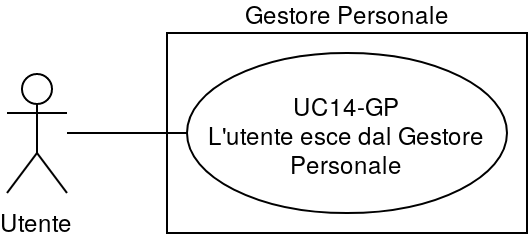
\includegraphics[width=\columnwidth]{img/casi_d'uso/UC14.png}\\
			\caption{UC\theuccount-GP - Inserimento utente}
		\end{figure}
	\begin{itemize}
		\item \textbf{Codice}: UC\theuccount-GP.
		\item \textbf{Titolo}: Inserimento utente.
		\item \textbf{Attori primari}: utente.
		\item \textbf{Descrizione}: l'utente, acceduto al sistema, aggiunge un nuovo utente nel sistema.
		Non è possibile che un utente non acceduto si iscriva da solo per la prima volta.
		In un primo momento è presente solo un utente predefinito che può aggiungere gli altri utenti.
		\item \textbf{Precondizione}: un nuovo utente deve essere aggiunto nel sistema.
		\item \textbf{Postcondizione}: un utente viene aggiunto al sistema.
		\item \textbf{Scenario principale}:
		\begin{enumerate}
			\item L'utente aggiunge un nuovo utente
		\end{enumerate}
	\end{itemize}
	%TODO:  aggiuora io, povero stronzo, che sono statonto.. come faccio a sapere qual è il mio identificativo?!
	\stepcounter{subuccount}
	\subsubsection{UC\theuccount.\thesubuccount-GP - Aggiunta nuovo utente}
		\begin{figure}[H]
			\centering
			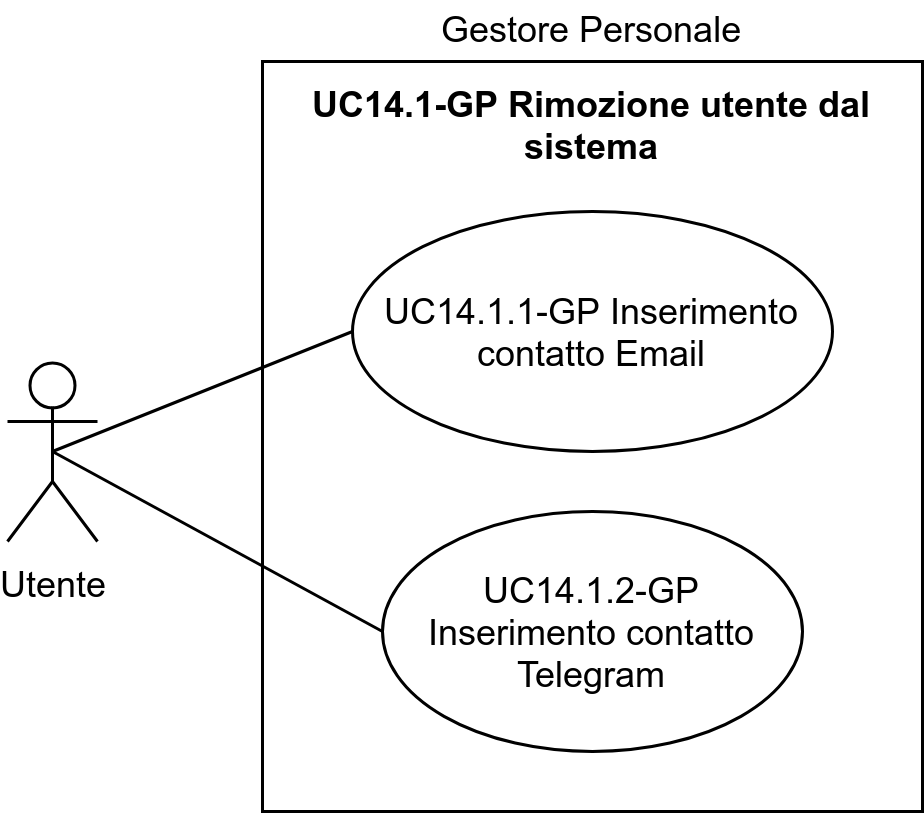
\includegraphics[width=\columnwidth]{img/casi_d'uso/UC14_1.png}\\
			\caption{UC\theuccount.\thesubuccount-GP - Aggiunta nuovo utente}
		\end{figure}
		\begin{itemize}
			\item \textbf{Codice}: C\theuccount.\thesubuccount-GP.
			\item \textbf{Titolo}: Aggiunta nuovo utente.
			\item \textbf{Attori primari}: utente.
			\item \textbf{Descrizione}: un nuovo utente viene inserito nel sistema.
			\item \textbf{Precondizione}: un nuovo utente deve essere aggiunto nel sistema.
			\item \textbf{Postcondizione}: un utente viene aggiunto al sistema.
			\item \textbf{Scenario principale}:
			\begin{enumerate}
				\item L'utente inserisce i dati del nuovo utente da aggiungere
				\item L'utente conferma l'invio dei dati
				\item L'aggiunta viene effettuata
			\end{enumerate}
			\item \textbf{Estensioni}:
			\begin{enumerate}
				\item Errore utente già presente nel sistema [UC\theuccount.2-GP]
			\end{enumerate}
		\end{itemize}

		\stepcounter{subsubuccount}
		\subsubsection{UC\theuccount.\thesubuccount.\thesubsubuccount-GP - Inserimento nome utente}

			\begin{itemize}
				\item \textbf{Codice}: UC\theuccount.\thesubuccount.\thesubsubuccount-GP.
				\item \textbf{Titolo}: inserimento nome utente.
				\item \textbf{Attori primari}: utente.
				%non registrato.
				\item \textbf{Descrizione}: l'utente inserisce il nominativo dell'utente da aggiungere.
				\item \textbf{Precondizione}: un nuovo utente deve essere aggiunto nel sistema.
				\item \textbf{Postcondizione}: il nome del nuovo utente è stato aggiunto nel sistema.
				\item \textbf{Scenario principale}:
				\begin{enumerate}
					\item L'utente aggiunge il nominativo del nuovo utente
				\end{enumerate}
			\end{itemize}

		\stepcounter{subsubuccount}
		\subsubsection{UC\theuccount.\thesubuccount.\thesubsubuccount-GP - Inserimento cognome utente}

			\begin{itemize}
				\item \textbf{Codice}: UC\theuccount.\thesubuccount.\thesubsubuccount-GP.
				\item \textbf{Titolo}: inserimento cognome utente.
				\item \textbf{Attori primari}: utente.
				% non registrato.
				\item \textbf{Descrizione}: l'utente inserisce il cognome dell'utente da aggiungere.
				\item \textbf{Precondizione}: un nuovo utente deve essere aggiunto nel sistema.
				\item \textbf{Postcondizione}: il cognome del nuovo utente è stato aggiunto nel sistema.
				\item \textbf{Scenario principale}:
				\begin{enumerate}
					\item L'utente aggiunge il cognome del nuovo utente
				\end{enumerate}
			\end{itemize}

		\stepcounter{subsubuccount}
		\subsubsection{UC\theuccount.\thesubuccount.\thesubsubuccount-GP - Inserimento contatto Email}

			\begin{itemize}
				\item \textbf{Codice}: UC\theuccount.\thesubuccount.\thesubsubuccount-GP.
				\item \textbf{Titolo}: inserimento contatto Email.
				\item \textbf{Attori primari}: utente.
				% non registrato.
				\item \textbf{Descrizione}: l'utente inserisce il contatto Email dell'utente da aggiungere.
				\item \textbf{Precondizione}: un nuovo utente deve essere aggiunto nel sistema.
				\item \textbf{Postcondizione}: il contatto Email è stato aggiunto.
				\item \textbf{Scenario principale}:
				\begin{enumerate}
					\item L'utente aggiunge il contatto Email del nuovo utente
				\end{enumerate}
		\end{itemize}

		\stepcounter{subsubuccount}
		\subsubsection{UC\theuccount.\thesubuccount.\thesubsubuccount-GP - Inserimento contatto Telegram}

			\begin{itemize}
				\item \textbf{Codice}: UC\theuccount.\thesubuccount.\thesubsubuccount-GP.
				\item \textbf{Titolo}: inserimento contatto Telegram.
				\item \textbf{Attori primari}: utente.
				% non registrato.
				\item \textbf{Descrizione}: l'utente inserisce il contatto Telegram dell'utente da aggiungere.
				\item \textbf{Precondizione}: un nuovo utente deve essere aggiunto nel sistema.
				\item \textbf{Postcondizione}: il contatto Telegram è stato aggiunto.
				\item \textbf{Scenario principale}:
				\begin{enumerate}
					\item L'utente aggiunge il contatto Telegram del nuovo utente
				\end{enumerate}
			\end{itemize}

	\stepcounter{subuccount}
	\subsubsection{UC\theuccount.\thesubuccount-GP - Errore utente già presente nel sistema}

		\begin{itemize}
			\item \textbf{Codice}: UC\theuccount.\thesubuccount-GP.
			\item \textbf{Titolo}: errore utente già presente nel sistema.
			\item \textbf{Attori primari}: utente.
			\item \textbf{Descrizione}: l’utente viene avvisato che i contatti Telegram o Email immessi non sono univoci.
			\item \textbf{Precondizione}: un nuovo utente deve essere aggiunto nel sistema.
			\item \textbf{Postcondizione}: il sistema comunica all’utilizzatore l’errore e l'utente non viene inserito.
			\item \textbf{Scenario principale}:
			\begin{enumerate}
				\item L'utente visualizza il messaggio d'errore
			\end{enumerate}
			\end{itemize}

\stepcounter{uccount}
%\clearpage
\subsubsection{UC\theuccount-GP - Rimozione preferenze}
		\begin{figure}[H]
			\centering
				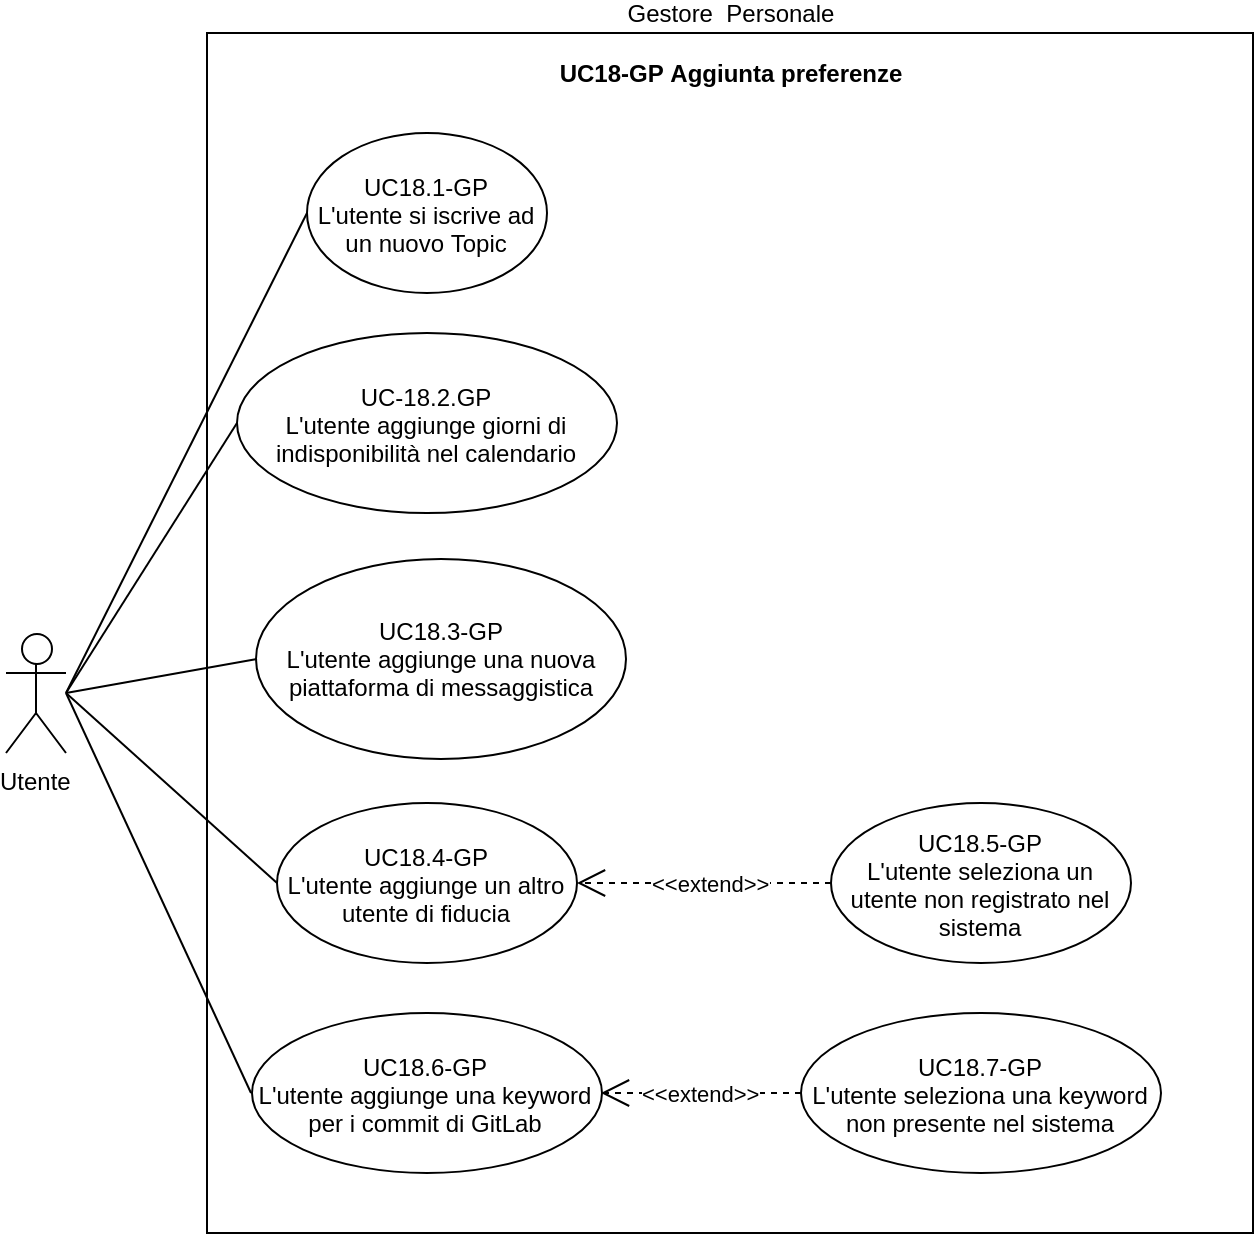
\includegraphics[width=\textwidth]{img/casi_d'uso/UC18.png}\\
			\caption{UC\theuccount-GP - Rimozione preferenze}
		\end{figure}
	\begin{itemize}
		\item \textbf{Codice}: UC\theuccount-GP.
		\item \textbf{Titolo}: rimozione preferenze.
		\item \textbf{Attori primari}: utente.
		\item \textbf{Descrizione}: l’utente, dopo aver selezionato delle preferenze dalle opzioni di configurazione, ne rimuove una o più. Le preferenze consistono in Topic, date di calendario e la piattaforma di messaggistica (Telegram e email).
		\item \textbf{Precondizione}: l’utente ha eseguito l'accesso nel sistema ed è presente almeno	una preferenza selezionata tra quelle proposte da Butterfly.
		\item \textbf{Postcondizione}: la nuova configurazione contiene una o più preferenze in meno rispetto	a quella precedente.
		\item \textbf{Scenario principale}:
		\begin{enumerate}
			\item L'utente procede alla rimozione di una o più preferenze
		\end{enumerate}
	\end{itemize}

	\stepcounter{subuccount}
	\subsubsection{UC\theuccount.\thesubuccount-GP - Disiscrizione Topic}

		\begin{itemize}
			\item \textbf{Codice}: UC\theuccount.\thesubuccount-GP.
			\item \textbf{Titolo}: disiscrizione Topic.
			\item \textbf{Attori primari}: utente.
			\item \textbf{Descrizione}: l’utente si disiscrive da uno o più Topic dai quali prima riceveva delle notifiche.
			\item \textbf{Precondizione}: l’utente ha acceduto correttamente nel sistema e non ha già selezionato tutti i Topic possibili proposti da \progetto.
			\item \textbf{Postcondizione}: il numero di Topic a cui è iscritto l’utente è diminuito.
			\item \textbf{Scenario principale}:
			\begin{enumerate}
				\item L'utente procede alla disiscrizione di uno o più Topic
			\end{enumerate}
		\end{itemize}

	\stepcounter{subuccount}
	\subsubsection{UC\theuccount.\thesubuccount-GP - Rimozione di uno o più giorni di irreperibilità nel calendario}

	\begin{itemize}
		\item \textbf{Codice}: UC\theuccount.\thesubuccount-GP.
		\item \textbf{Titolo}: rimozione di uno o più giorni di irreperibilità nel calendario.
		\item \textbf{Attori primari}: utente.
		\item \textbf{Descrizione}: l’utente rimuove i giorni di calendario in cui precedentemente	non era reperibile, tornando disponibile.
		\item \textbf{Precondizione}: l’utente ha acceduto correttamente nel sistema ed è presente almeno un giorno di calendario selezionato.
		\item \textbf{Postcondizione}: il numero di giorni di calendario in cui l’utente non è reperibile è diminuito.
		\item \textbf{Scenario principale}:
		\begin{enumerate}
			\item L'utente procede alla rimozione di uno o più giorni di irreperibilità
		\end{enumerate}
	\end{itemize}

	\stepcounter{subuccount}
	\subsubsection{UC\theuccount.\thesubuccount-GP - Rimozione preferenza piattaforma di messaggistica}

	\begin{itemize}
		\item \textbf{Codice}: UC\theuccount.\thesubuccount-GP.
		\item \textbf{Titolo}: rimozione preferenza piattaforma di messaggistica.
		\item \textbf{Attori primari}: utente.
		\item \textbf{Descrizione}: l’utente rimuove una o più preferenze tra Telegram e Email dalle	quali non vuole più ricevere notifiche tramite \progetto.
		\item \textbf{Precondizione}: l’utente ha acceduto correttamente nel sistema ed è presente almeno una piattaforma di messaggistica selezionata tra quelle proposte da \progetto.
		\item \textbf{Postcondizione}: il numero di piattaforme di messaggistica da cui l’utente vuole ricevere notifiche è diminuito.
		\item \textbf{Scenario principale}:
		\begin{enumerate}
			\item L'utente procede alla rimozione di una o più piattaforme di messaggistica
		\end{enumerate}
	\end{itemize}

	% \stepcounter{subuccount}
	% \subsubsection{UC\theuccount.\thesubuccount-GP - Rimozione persona di fiducia}

	% \begin{itemize}
	% 	\item \textbf{Codice}: UC\theuccount.\thesubuccount-GP.
	% 	\item \textbf{Titolo}: aggiunta persona di fiducia.
	% 	\item \textbf{Attori primari}: utente.
	% 	\item \textbf{Descrizione}:  l’utente rimuove l'utente legato a un identificativo di sua preferenza a cui inoltrare i messaggi in caso di indisponibilità.
	% 	\item \textbf{Precondizione}: l’utente ha eseguito l'accesso nel sistema e vuole rimuovere la sua persona di fiducia.
	% 	\item \textbf{Postcondizione}: la preferenza viene rimossa correttamente.
	% 	\item \textbf{Scenario principale}:
	% 	\begin{enumerate}
	% 		\item L’utente procede alla rimozione della sua persona di fiducia
	% 	\end{enumerate}
	% 	\item \textbf{Estensioni}:
	% 	\begin{enumerate}
	% 		\item Errore identificativo persona di fiducia inesistente [UC\theuccount.5-GP].
	% 	\end{enumerate}
	% \end{itemize}

	% \stepcounter{subuccount}
	% \subsubsection{UC\theuccount.\thesubuccount-GP - Errore identificativo persona di fiducia inesistente}

	% \begin{itemize}
	% 	\item \textbf{Codice}: UC\theuccount.\thesubuccount-GP.
	% 	\item \textbf{Titolo}: errore identificativo persona di fiducia inesistente.
	% 	\item \textbf{Attori primari}: utente.
	% 	\item \textbf{Descrizione}: l’utente viene avvisato che ha inserito un identificativo errato.
	% 	\item \textbf{Precondizione}: l’utente ha acceduto con le sue credenziali corrette nel sistema e vuole rimuovere la sua persona di fiducia.
	% 	\item \textbf{Postcondizione}: il sistema comunica all’utilizzatore l’errore.
	% 	\item \textbf{Scenario principale}:
	% 	\begin{enumerate}
	% 		\item L'utente inserisce l'identificativo della sua persona di fiducia
	% 		\item Il sistema rileva che questo identificativo non esiste
	% 		\item L'utente visualizza il messaggio di errore
	% 	\end{enumerate}
	% \end{itemize}

	\stepcounter{subuccount}
	\subsubsection{UC\theuccount.\thesubuccount-GP - Rimozione di keyword per i push di GitLab}

	\begin{itemize}
		\item \textbf{Codice}: UC\theuccount.\thesubuccount-GP.
		\item \textbf{Titolo}: rimozione di keyword per i push di GitLab.
		\item \textbf{Attori primari}: utente.
		\item \textbf{Descrizione}: l’utente seleziona e rimuove una o più keyword già presente nel sistema per non ricevere la notifica di push in
		cui i messaggi di commit contengono la keyword rimossa.
		\item \textbf{Precondizione}:  l’utente ha acceduto al sistema.
		\item \textbf{Postcondizione}: nelle nuove configurazioni dell'utente selezionato sono state rimosse delle keyword precedentemente presenti.
		\item \textbf{Scenario principale}:
		\begin{enumerate}
			\item L'utente rimuove una o più keyword per cui non vuole iù ricevere messaggi di push
		\end{enumerate}
		\item \textbf{Estensioni}:
		\begin{enumerate}
			\item Errore keyword da rimuovere non presente [UC\theuccount.7-GP]
		\end{enumerate}
	\end{itemize}

	\stepcounter{subuccount}
	\subsubsection{UC\theuccount.\thesubuccount-GP - Errore keyword da rimuovere non presente}

	\begin{itemize}
		\item \textbf{Codice}: UC\theuccount.\thesubuccount-GP.
		\item \textbf{Titolo}: errore keyword da rimuovere non presente.
		\item \textbf{Attori primari}: utente.
		\item \textbf{Descrizione}: l'utente vuole rimuovere una keyword che non ha mai inserito o che ha rimosso precedentemente.
		\item \textbf{Precondizione}: l’utente ha acceduto al sistema.
		\item \textbf{Postcondizione}: viene visualizzato un messaggio d'errore con indicato che la keyword	selezionata che non è presente nel sistema.
		\item \textbf{Scenario principale}:
		\begin{enumerate}
			\item L'utente inserisce la keyword che vuole rimuovere
			\item Il sistema rileva che non è presente
			\item L'utente visualizza il messaggio di errore
		\end{enumerate}
	\end{itemize}


\stepcounter{uccount}
%\clearpage
\subsubsection{UC\theuccount-GP - Modifica utente}
		\begin{figure}[H]
			\centering
				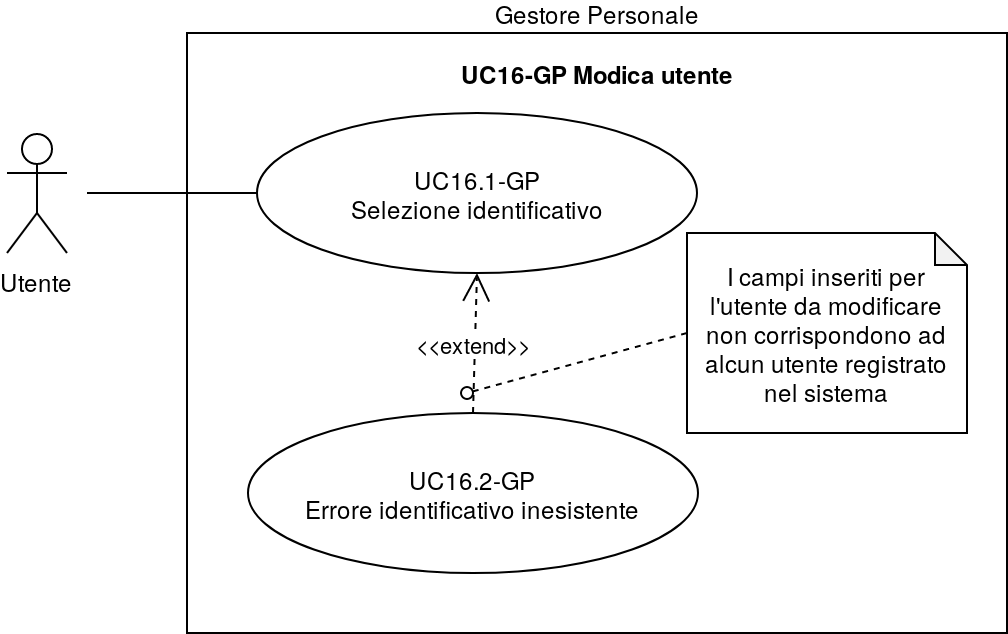
\includegraphics[width=0.8\textwidth]{img/casi_d'uso/UC16.png}\\
			\caption{UC\theuccount-GP - Modifica utente}
		\end{figure}
	\begin{itemize}
		\item \textbf{Codice}: UC\theuccount-GP.
		\item \textbf{Titolo}: modifica utente.
		\item \textbf{Attori primari}: utente.
		\item \textbf{Descrizione}: l’utente vuole modificare le informazioni relative a un altro utente, o di se stesso.
		\item \textbf{Precondizione}: l'utente vuole modificare i dati di un utente già presente nel sistema.
		\item \textbf{Postcondizione}: i campi dell'utente sono stati modificati correttamente.
		\item \textbf{Scenario Principale}:
		\begin{enumerate}
			\item L'utente modifica i dati relativi di un utente
		\end{enumerate}
	\end{itemize}
	
	\stepcounter{subuccount}
	\subsubsection{UC\theuccount.\thesubuccount-GP - Selezione identificativo}
		\begin{figure}[H]
			\centering
			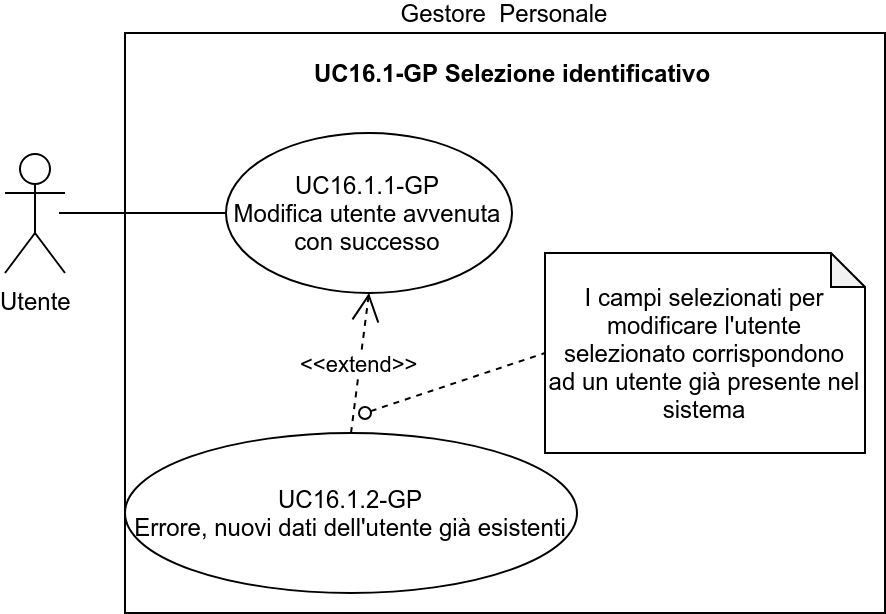
\includegraphics[width=0.8\textwidth]{img/casi_d'uso/UC16_1.png}\\
			\caption{UC\theuccount.\thesubuccount-GP - Selezione identificativo}
		\end{figure}
		\begin{itemize}
			\item \textbf{Codice}: UC\theuccount.\thesubuccount-GP.
			\item \textbf{Titolo}: selezione identificativo.
			\item \textbf{Attori primari}: utente.
			\item \textbf{Descrizione}: l'utente aggiunge l'identificativo dell'utente che vuole modificare.
			\item \textbf{Precondizione}: l'utente vuole modificare un utente già presente.
			\item \textbf{Postcondizione}: l'identificativo è stato inserito.
			\item \textbf{Scenario Principale}:
			\begin{enumerate}
				\item L'utente procede con l'inserimento dell'identificativo dell'utente da modificare
			\end{enumerate}
			\item \textbf{Estensioni}:
			\begin{itemize}
				\item Errore identificativo inesistente [UC\theuccount.2-GP]
			\end{itemize}
		\end{itemize}
		
		\stepcounter{subsubuccount}
		\subsubsection{UC\theuccount.\thesubuccount.\thesubsubuccount-GP - Modifica utente avvenuta con successo}
			\begin{figure}[H]
				\centering
				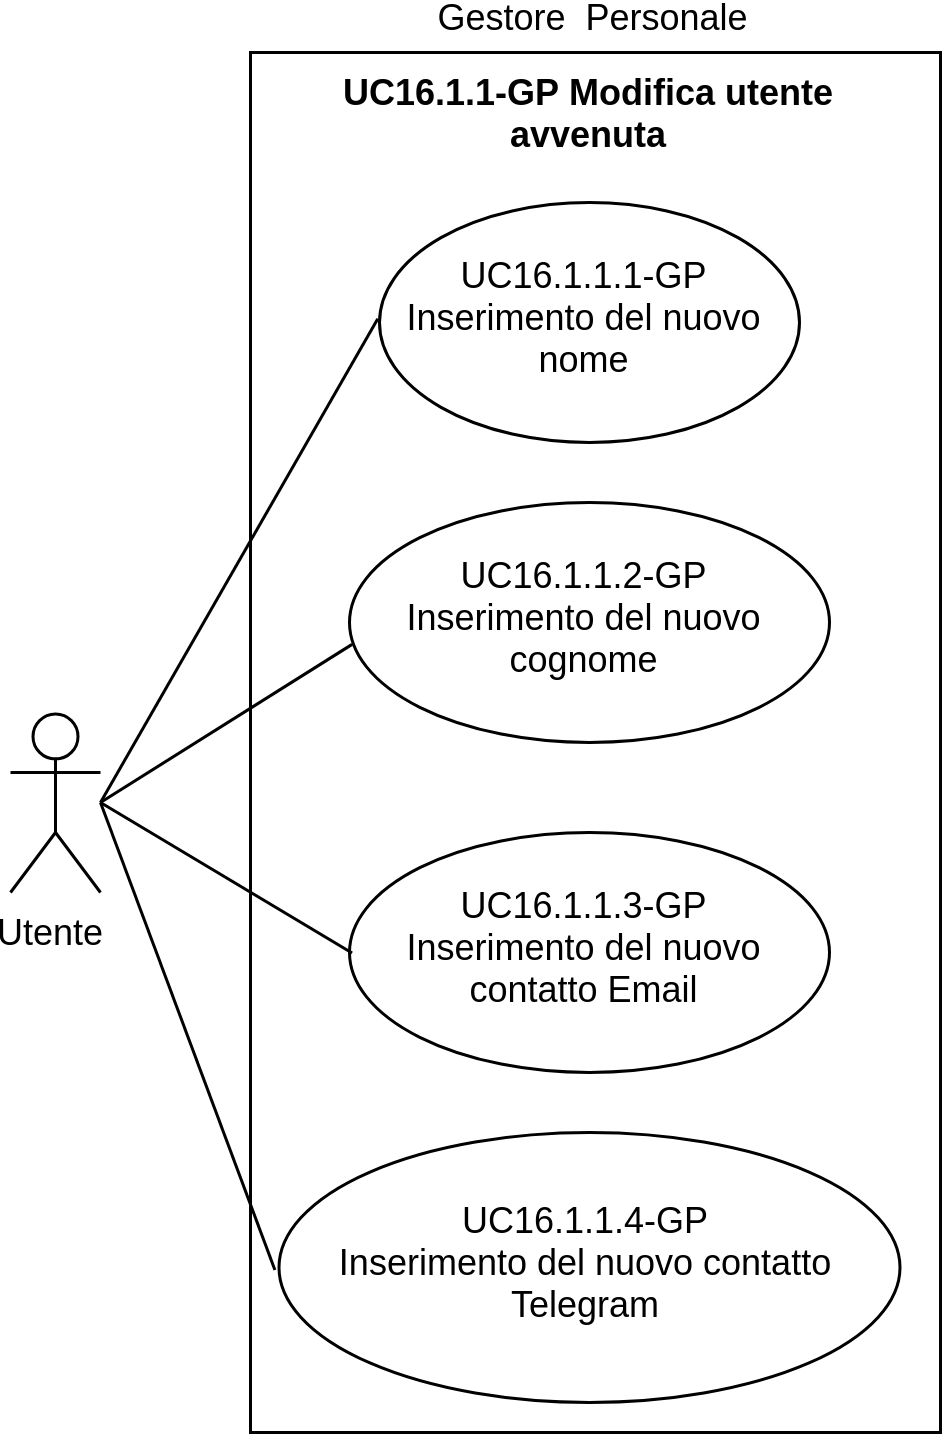
\includegraphics[width=0.5\columnwidth]{img/casi_d'uso/UC16_1_1.png}\\
				\caption{UC\theuccount.\thesubuccount.\thesubsubuccount-GP - Modifica utente avvenuta con successo}
			\end{figure}
			\begin{itemize}
				\item \textbf{Codice}: UC\theuccount.\thesubuccount.\thesubsubuccount-GP.
				\item \textbf{Titolo}: modifica utente avvenuta con successo.
				\item \textbf{Attori primari}: utente.
				\item \textbf{Descrizione}: l'identificativo è presente nel sistema e ne vengono modificati i relativi campi con successo.
				\item \textbf{Precondizione}: l'utente vuole modificare un utente già presente.
				\item \textbf{Postcondizione}: l'utente è stato modificato con successo.
				\item \textbf{Scenario Principale}:
				\begin{enumerate}
					\item L'utente viene modificato con successo
				\end{enumerate}
				\item \textbf{Estensioni}:
				\begin{itemize}
					\item Errore, nuovi dati dell'utente già esistenti [UC\theuccount.\thesubuccount.2-GP]
				\end{itemize}
			\end{itemize}
			
			\stepcounter{subsubsubuccount}
			\subsubsection{UC\theuccount.\thesubuccount.\thesubsubuccount.\thesubsubsubuccount-GP - Inserimento del nuovo nome}
				
				\begin{itemize}
					\item \textbf{Codice}: UC\theuccount.\thesubuccount.\thesubsubuccount.\thesubsubsubuccount-GP.
					\item \textbf{Titolo}: inserimento del nuovo nome.
					\item \textbf{Attori primari}: utente.
					\item \textbf{Descrizione}: l'utente aggiunge il nuovo nome relativo all'identificativo inserito che vuole modificare.
					\item \textbf{Precondizione}: l'utente vuole modificare un utente già presente.
					\item \textbf{Postcondizione}: il nome è stato inserito.
					\item \textbf{Scenario Principale}:
					\begin{enumerate}
						\item L'utente inserisce il nuovo nome dell'utente che vuole modificare
					\end{enumerate}
				\end{itemize}
			
			\stepcounter{subsubsubuccount}
			\subsubsection{UC\theuccount.\thesubuccount.\thesubsubuccount.\thesubsubsubuccount-GP - Inserimento del nuovo cognome}
				
				\begin{itemize}
					\item \textbf{Codice}: UC\theuccount.\thesubuccount.\thesubsubuccount.\thesubsubsubuccount-GP.
					\item \textbf{Titolo}: inserimento del nuovo cognome.
					\item \textbf{Attori primari}: utente.
					\item \textbf{Descrizione}: l'utente aggiunge il nuovo cognome relativo all'identificativo inserito che vuole modificare.
					\item \textbf{Precondizione}: l'utente vuole modificare un utente già presente.
					\item \textbf{Postcondizione}: il cognome è stato inserito.
					\item \textbf{Scenario Principale}:
					\begin{enumerate}
						\item L'utente inserisce il nuovo cognome dell'utente che vuole modificare.
					\end{enumerate}
				\end{itemize}
			
			\stepcounter{subsubsubuccount}
			\subsubsection{UC\theuccount.\thesubuccount.\thesubsubuccount.\thesubsubsubuccount-GP - Inserimento del nuovo contatto Email}
				
				\begin{itemize}
					\item \textbf{Codice}: UC\theuccount.\thesubuccount.\thesubsubuccount.\thesubsubsubuccount-GP.
					\item \textbf{Titolo}: inserimento del nuovo contatto Email.
					\item \textbf{Attori primari}: utente.
					\item \textbf{Descrizione}: l'utente aggiunge il nuovo contatto Email relativo all'identificativo inserito che vuole modificare.
					\item \textbf{Precondizione}: l'utente vuole modificare un utente già presente.
					\item \textbf{Postcondizione}: il contatto Email è stato inserito.
					\item \textbf{Scenario Principale}:
					\begin{enumerate}
						\item L'utente inserisce il nuovo contatto Email dell'utente che vuole modificare
					\end{enumerate}
				\end{itemize}
			
			\stepcounter{subsubsubuccount}
			\subsubsection{UC\theuccount.\thesubuccount.\thesubsubuccount.\thesubsubsubuccount-GP - Inserimento del nuovo contatto Telegram}
				
				\begin{itemize}
					\item \textbf{Codice}: UC\theuccount.\thesubuccount.\thesubsubuccount.\thesubsubsubuccount-GP.
					\item \textbf{Titolo}: inserimento del nuovo contatto Telegram.
					\item \textbf{Attori primari}: utente.
					\item \textbf{Descrizione}: l'utente aggiunge il nuovo contatto Telegram relativo all'identificativo inserito che vuole modificare.
					\item \textbf{Precondizione}: l'utente vuole modificare un utente già presente.
					\item \textbf{Postcondizione}: il contatto Telegram è stato inserito.
					\item \textbf{Scenario Principale}:
					\begin{enumerate}
						\item L'utente inserisce il nuovo contatto Telegram dell'utente che vuole modificare
					\end{enumerate}
				\end{itemize}
			
		\stepcounter{subsubuccount}
		\subsubsection{UC\theuccount.\thesubuccount.\thesubsubuccount-GP - Errore, nuovi dati dell'utente già esistenti}
		
		\begin{itemize}
			\item \textbf{Codice}: UC\theuccount.\thesubuccount.\thesubsubuccount-GP.
			\item \textbf{Titolo}: errore, nuovi dati dell'utente già esistenti.
			\item \textbf{Attori primari}: utente.
			\item \textbf{Descrizione}: i nuovi dati dell'utente da modificare che sono stati inseriti sono già presenti nel sistema.
			\item \textbf{Precondizione}: l'utente vuole modificare un utente già presente.
			\item \textbf{Postcondizione}: l'utente non è stato modificato.
			\item \textbf{Scenario Principale}:
			\begin{enumerate}
				\item L'utente non viene modificato perché i nuovi campi corrispondono a quelli di un utente già esistente
			\end{enumerate}
		\end{itemize}
	\stepcounter{subuccount}
	\subsubsection{UC\theuccount.\thesubuccount-GP - Errore identificativo inesistente}
		
		\begin{itemize}
			\item \textbf{Codice}: UC\theuccount.\thesubuccount-GP.
			\item \textbf{Titolo}: errore identificativo inesistente.
			\item \textbf{Attori primari}: utente.
			\item \textbf{Descrizione}:  l’utente viene avvisato che ha inserito un'identificativo errato.
			\item \textbf{Precondizione}: l'utente vuole modificare un utente già presente.
			\item \textbf{Postcondizione}: il sistema comunica all’utilizzatore l’errore.
			\item \textbf{Scenario Principale}:
			\begin{enumerate}
				\item L'utente ha inserito un identificativo errato e il sistema comunica all’utilizzatore l’errore.
			\end{enumerate}
		\end{itemize}

\stepcounter{uccount}
%\clearpage
\subsubsection{UC\theuccount-GP - Aggiunta preferenze}
		\begin{figure}[H]
			\centering
				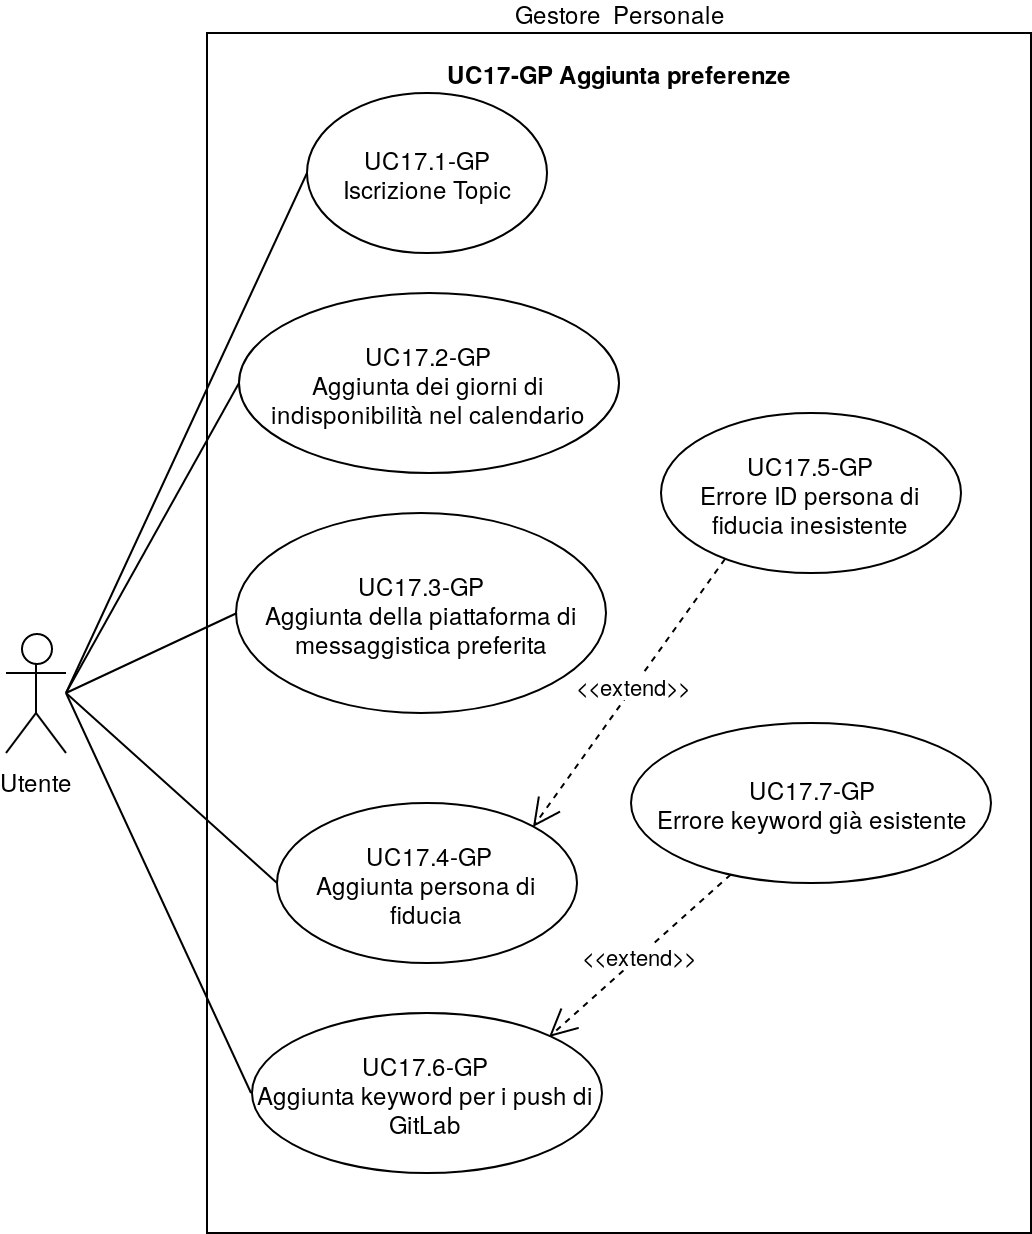
\includegraphics[width=1\textwidth]{img/casi_d'uso/UC17.png}\\
			\caption{UC\theuccount-GP - Aggiunta preferenze}
		\end{figure}
	\begin{itemize}
		\item \textbf{Codice}: UC\theuccount-GP.
		\item \textbf{Titolo}: aggiunta preferenze.
		\item \textbf{Attori primari}: utente.
		\item \textbf{Descrizione}: l’utente, date le varie opzioni per configurare Butterfly, aggiunge una
		preferenza tra Topic, giorni di calendario, piattaforma di messaggistica (Telegram o Email)	preferita e la persona di fiducia che lo può sostituire.
		\item \textbf{Precondizione}: l’utente ha acceduto con le sue credenziali corrette nel sistema e non ha già selezionato tutte le preferenze possibili proposte da \progetto.
		\item \textbf{Postcondizione}: la nuova configurazione contiene una o più preferenze in aggiunta rispetto a quella precedente.
		\item \textbf{Scenario principale}:
		\begin{enumerate}
			\item L'utente aggiunge una o più preferenze
		\end{enumerate}
	\end{itemize}

	\stepcounter{subuccount}
	\subsubsection{UC\theuccount.\thesubuccount-GP - Iscrizione Topic}

		\begin{itemize}
			\item \textbf{Codice}: UC\theuccount.\thesubuccount-GP.
			\item \textbf{Titolo}: iscrizione Topic.
			\item \textbf{Attori primari}: utente.
			\item \textbf{Descrizione}: data la lista di Topic presenti, l’utente ne seleziona uno o	più a cui è interessato, ricevendone una notifica. I Topic sono divisi per categoria e	comprendono etichette, progetto a cui sono legate e l'applicazione di provenienza: Redmine o GitLab.
			\item \textbf{Precondizione}: l’utente ha acceduto correttamente nel sistema e non ha già selezionato tutti i Topic possibili proposti da \progetto.
			\item \textbf{Postcondizione}: il numero di Topic a cui è interessato l’utente è aumentato.
			\item \textbf{Scenario principale}:
			\begin{enumerate}
				\item L'utente procede all'iscrizione di uno o più Topic
			\end{enumerate}
		\end{itemize}
	
	\stepcounter{subuccount}
	\subsubsection{UC\theuccount.\thesubuccount-GP - Aggiunta dei giorni di indisponibilità nel calendario}
		
		\begin{itemize}
			\item \textbf{Codice}: UC\theuccount.\thesubuccount-GP.
			\item \textbf{Titolo}: aggiunta dei giorni di indisponibilità nel calendario.
			\item \textbf{Attori primari}: utente.
			\item \textbf{Descrizione}: dato il calendario lavorativo, l’utente aggiunge uno o più giorni in cui non è reperibile e non vuole ricevere notifiche.
			\item \textbf{Precondizione}: l’utente ha acceduto correttamente nel sistema e vuole selezionare alcuni giorni di indisponibilità.
			\item \textbf{Postcondizione}: il numero di giorni in cui l’utente non si rende disponibile è aumentato.
			\item \textbf{Scenario principale}:
			\begin{enumerate}
				\item L'utente procede all'inserimento di uno o più giorni di indisponibilità
			\end{enumerate}
		\end{itemize}
	
	\stepcounter{subuccount}
	\subsubsection{UC\theuccount.\thesubuccount-GP - Aggiunta della piattaforma di messaggistica preferita}
		
		\begin{itemize}
			\item \textbf{Codice}: UC\theuccount.\thesubuccount-GP.
			\item \textbf{Titolo}: aggiunta della piattaforma di messaggistica preferita.
			\item \textbf{Attori primari}: utente.
			\item \textbf{Descrizione}: l’utente aggiunge la sua preferenza tra Telegram e Email dove vuole ricevere le notifiche.
			\item \textbf{Precondizione}: l’utente ha acceduto correttamente nel sistema e non ha già selezionato tutte le piattaforme di messaggistica possibili proposte da \progetto.
			\item \textbf{Postcondizione}: il numero di piattaforme di messaggistica selezionate dall’utente è aumentato.
			\item \textbf{Scenario principale}:
			\begin{enumerate}
				\item L'utente procede all'aggiunta di una o più piattaforme di messaggistica
			\end{enumerate}
		\end{itemize}
	
	\stepcounter{subuccount}
	\subsubsection{UC\theuccount.\thesubuccount-GP - Aggiunta persona di fiducia}
		
		\begin{itemize}
			\item \textbf{Codice}: UC\theuccount.\thesubuccount-GP.
			\item \textbf{Titolo}: aggiunta persona di fiducia.
			\item \textbf{Attori primari}: utente.
			\item \textbf{Descrizione}: l’utente aggiunge l'utente legato a un identificativo di sua preferenza a cui inoltrare i messaggi in caso di indisponibilità.
			\item \textbf{Precondizione}: l’utente ha acceduto con le sue credenziali corrette nel sistema e non ha già selezionato la persona a cui inoltrare le notifiche.
			\item \textbf{Postcondizione}: la preferenza viene aggiunta correttamente.
			\item \textbf{Scenario principale}:
			\begin{enumerate}
				\item L'utente procede all'aggiunta della sua persona di fiducia
			\end{enumerate}
			\item \textbf{Estensioni}:
			\begin{enumerate}
				\item Errore identificativo persona di fiducia inesistente [UC\theuccount.5-GP]
			\end{enumerate}
		\end{itemize}
	
	\stepcounter{subuccount}
	\subsubsection{UC\theuccount.\thesubuccount-GP - Errore identificativo persona di fiducia inesistente}
		
		\begin{itemize}
			\item \textbf{Codice}: UC\theuccount.\thesubuccount-GP.
			\item \textbf{Titolo}: errore identificativo persona di fiducia inesistente.
			\item \textbf{Attori primari}: utente.
			\item \textbf{Descrizione}: l’utente cerca di aggiungere una persona di fiducia ma viene avvisato che ha inserito un identificativo errato.
			\item \textbf{Precondizione}: l’utente ha acceduto con le sue credenziali corrette nel sistema e non ha già selezionato la persona a cui inoltrare le notifiche.
			\item \textbf{Postcondizione}: il sistema comunica all’utilizzatore l’errore di preferenza.
			\item \textbf{Scenario principale}:
			\begin{enumerate}
				\item L'utente procede all'aggiunta della sua persona di fiducia
				\item Il sistema rileva che la persona di fiducia non esiste
				\item L'utente visualizza l'errore
			\end{enumerate}
		\end{itemize}
	
	\stepcounter{subuccount}
	\subsubsection{UC\theuccount.\thesubuccount-GP - Aggiunta keyword per i push di GitLab}
		
		\begin{itemize}
			\item \textbf{Codice}: UC\theuccount.\thesubuccount-GP.
			\item \textbf{Titolo}: aggiunta keyword per i push di GitLab.
			\item \textbf{Attori primari}: utente.
			\item \textbf{Descrizione}: l’utente aggiunge le keyword che vuole che siano contenute nei messaggi di commit dei push di cui vuole ricevere la notifica.
			\item \textbf{Precondizione}: l’utente ha acceduto al sistema.
			\item \textbf{Postcondizione}: nelle nuove configurazioni dell'utente selezionato sono presenti una o più nuove keyword per ricevere le notifiche da push di GitLab di interesse.
			\item \textbf{Scenario principale}:
			\begin{enumerate}
				\item L'utente procede all'aggiunta di una o più nuove keyword
			\end{enumerate}
			\item \textbf{Estensioni}:
			\begin{enumerate}
				\item Errore keyword già esistente [UC\theuccount.7-GP]
			\end{enumerate}
		\end{itemize}
	
	\stepcounter{subuccount}
	\subsubsection{UC\theuccount.\thesubuccount-GP - Errore keyword già esistente}
	
	\begin{itemize}
		\item \textbf{Codice}: UC\theuccount.\thesubuccount-GP.
		\item \textbf{Titolo}: errore keyword già esistente.
		\item \textbf{Attori primari}: utente.
		\item \textbf{Descrizione}: la keyword che vuole aggiungere l'utente è già registrata nel sistema.
		\item \textbf{Precondizione}:  l’utente ha acceduto al sistema.
		\item \textbf{Postcondizione}: il sistema comunica all’utilizzatore l’errore della keyword.
		\item \textbf{Scenario principale}:
		\begin{enumerate}
			\item L'utente procede all'aggiunta di keyword
			\item Il sistema rileva che queste sono già presenti
			\item L'utente visualizza un messaggio di errore
		\end{enumerate}
	\end{itemize}

\stepcounter{uccount}
%\clearpage
\subsubsection{UC\theuccount-GP - Rimozione preferenze}
		\begin{figure}[H]
			\centering
				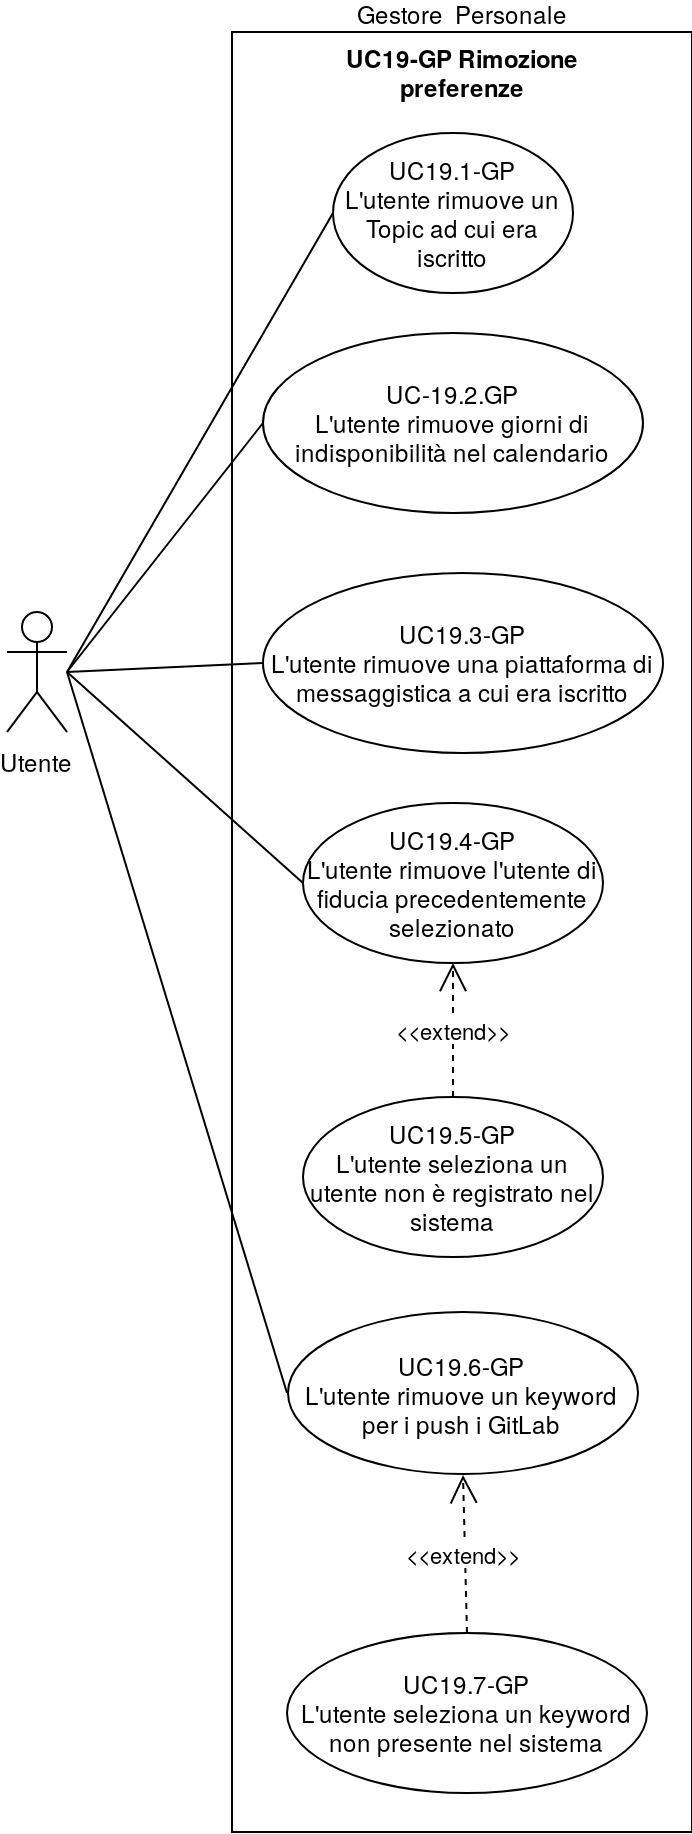
\includegraphics[width=\textwidth]{img/casi_d'uso/UC19.png}\\
			\caption{UC\theuccount-GP - Rimozione preferenze}
		\end{figure}
	\begin{itemize}
		\item \textbf{Codice}: UC\theuccount-GP.
		\item \textbf{Titolo}: rimozione preferenze.
		\item \textbf{Attori primari}: utente.
		\item \textbf{Descrizione}: l’utente, dopo aver selezionato delle preferenze dalle opzioni di configurazione, ne rimuove una o più. Le preferenze consistono in Topic, date di calendario, piattaforma di messaggistica (Telegram e email) e persona di fiducia che lo può sostituire.
		\item \textbf{Precondizione}: l’utente ha eseguito l'accesso nel sistema ed è presente almeno	una preferenza selezionata tra quelle proposte da Butterfly.
		\item \textbf{Postcondizione}: la nuova configurazione contiene una o più preferenze in meno rispetto	a quella precedente.
		\item \textbf{Scenario Principale}:
		\begin{enumerate}
			\item L'utente procede alla rimozione di una o più preferenze
		\end{enumerate}
	\end{itemize}

	\stepcounter{subuccount}
	\paragraph{UC\theuccount.\thesubuccount-GP - Disiscrizione Topic}
		
		\begin{itemize}
			\item \textbf{Codice}: UC\theuccount.\thesubuccount-GP.
			\item \textbf{Titolo}: disiscrizione Topic.
			\item \textbf{Attori primari}: utente.
			\item \textbf{Descrizione}: l’utente si disiscrive da uno o più Topic dai quali prima riceveva delle notifiche.
			\item \textbf{Precondizione}: l’utente ha acceduto correttamente nel sistema e non ha già selezionato tutti i Topic possibili proposti da \progetto.
			\item \textbf{Postcondizione}: il numero di Topic a cui è iscritto l’utente è diminuito.
			\item \textbf{Scenario Principale}:
			\begin{enumerate}
				\item L'utente procede alla disiscrizione di uno o più Topic
			\end{enumerate}
		\end{itemize}
	
	\stepcounter{subuccount}
	\paragraph{UC\theuccount.\thesubuccount-GP - Rimozione di uno o più giorni di irreperibilità nel calendario}
	
	\begin{itemize}
		\item \textbf{Codice}: UC\theuccount.\thesubuccount-GP.
		\item \textbf{Titolo}: rimozione di uno o più giorni di irreperibilità nel calendario.
		\item \textbf{Attori primari}: utente.
		\item \textbf{Descrizione}: l’utente rimuove i giorni di calendario in cui precedentemente	non era reperibile, tornando disponibile.
		\item \textbf{Precondizione}: l’utente ha acceduto correttamente nel sistema ed è presente almeno un giorno di calendario selezionato tra quelli proposti da \progetto.
		\item \textbf{Postcondizione}: il numero di giorni di calendario in cui l’utente non è reperibile è diminuito.
		\item \textbf{Scenario Principale}:
		\begin{enumerate}
			\item L'utente procede alla rimozione di uno o più giorni di irreperibilità
		\end{enumerate}
	\end{itemize}
	
	\stepcounter{subuccount}
	\paragraph{UC\theuccount.\thesubuccount-GP - Rimozione preferenza piattaforma di messaggistica}
	
	\begin{itemize}
		\item \textbf{Codice}: UC\theuccount.\thesubuccount-GP.
		\item \textbf{Titolo}: rimozione preferenza piattaforma di messaggistica.
		\item \textbf{Attori primari}: utente.
		\item \textbf{Descrizione}: l’utente rimuove una o più preferenze tra Telegram e Email dalle	quali non vuole più ricevere notifiche tramite \progetto.
		\item \textbf{Precondizione}: l’utente ha acceduto correttamente nel sistema ed è presente almeno una piattaforma di messaggistica selezionata tra quelle proposte da \progetto.
		\item \textbf{Postcondizione}: il numero di piattaforme di messaggistica da cui l’utente vuole ricevere notifiche è diminuito.
		\item \textbf{Scenario Principale}:
		\begin{enumerate}
			\item L'utente procede alla rimozione di una o più piattaforme di messaggistica
		\end{enumerate}
	\end{itemize}
	
	\stepcounter{subuccount}
	\paragraph{UC\theuccount.\thesubuccount-GP - Rimozione persona di fiducia}
	
	\begin{itemize}
		\item \textbf{Codice}: UC\theuccount.\thesubuccount-GP.
		\item \textbf{Titolo}: aggiunta persona di fiducia.
		\item \textbf{Attori primari}: utente.
		\item \textbf{Descrizione}:  l’utente rimuove l'utente legato a un ID di sua preferenza a cui inoltrare i messaggi in caso di indisponibilità.
		\item \textbf{Precondizione}: l’utente ha eseguito l'accesso nel sistema ed è presente almeno uno user con l'ID selezionato tra quelle proposte da \progetto.
		\item \textbf{Postcondizione}: la preferenza viene rimossa correttamente.
		\item \textbf{Scenario Principale}:
		\begin{enumerate}
			\item L'utente procede alla rimozione della sua persona di fiducia
		\end{enumerate}
		\item \textbf{Estensioni}:
		\begin{enumerate}
			\item Errore ID persona di fiducia inesistente [UC\theuccount.5-GP].
		\end{enumerate}
	\end{itemize}
	
	\stepcounter{subuccount}
	\paragraph{UC\theuccount.\thesubuccount-GP - Errore ID persona di fiducia inesistente}
	
	\begin{itemize}
		\item \textbf{Codice}: UC\theuccount.\thesubuccount-GP.
		\item \textbf{Titolo}: errore ID persona di fiducia inesistente.
		\item \textbf{Attori primari}: utente.
		\item \textbf{Descrizione}: l’utente viene avvisato che ha inserito un identificativo errato.
		\item \textbf{Precondizione}: l’utente ha acceduto con le sue credenziali corrette nel sistema e non ha già selezionato la persona a cui inoltrare le notifiche.
		\item \textbf{Postcondizione}: il sistema comunica all’utilizzatore l’errore di preferenza.
		\item \textbf{Scenario Principale}:
		\begin{enumerate}
			\item L'utente procede alla rimozione della sua persona di fiducia, questa però non esiste e
			visualizza l'errore
		\end{enumerate}
	\end{itemize}

	\stepcounter{subuccount}
	\paragraph{UC\theuccount.\thesubuccount-GP - Rimozione con successo di keyword per i push di GitLab}
	
	\begin{itemize}
		\item \textbf{Codice}: UC\theuccount.\thesubuccount-GP.
		\item \textbf{Titolo}: rimozione con successo di keyword per i push di GitLab.
		\item \textbf{Attori primari}: utente.
		\item \textbf{Descrizione}: l’utente seleziona e rimuove una o più keyword già presente nel sistema per non ricevere la notifica di push in
		cui i messaggi di commit contengono la keyword rimossa.
		\item \textbf{Precondizione}:  l’utente ha acceduto con le sue credenziali corrette nel sistema.
		\item \textbf{Postcondizione}: nelle nuove configurazioni dell'utente selezionato sono state rimosse delle keyword precedentemente presenti.
		\item \textbf{Scenario Principale}:
		\begin{enumerate}
			\item L'utente rimuove con successo una o più keyword per cui non vuole iù ricevere messaggi di push
		\end{enumerate}
		\item \textbf{Estensioni}:
		\begin{enumerate}
			\item Errore keyword da rimuovere non presente [UC\theuccount.7-GP]
		\end{enumerate}
	\end{itemize}
	
	\stepcounter{subuccount}
	\paragraph{UC\theuccount.\thesubuccount-GP - Errore keyword da rimuovere non presente}
	
	\begin{itemize}
		\item \textbf{Codice}: UC\theuccount.\thesubuccount-GP.
		\item \textbf{Titolo}: errore keyword da rimuovere non presente.
		\item \textbf{Attori primari}: utente.
		\item \textbf{Descrizione}: la keyword che l'utente intende rimuovere non è registrata nel sistema.
		\item \textbf{Precondizione}: l’utente ha acceduto con le sue credenziali corrette nel sistema.
		\item \textbf{Postcondizione}: viene visualizzato un messaggio d'errore con indicato che la keyword	selezionata che non è presente nel sistema.
		\item \textbf{Scenario Principale}:
		\begin{enumerate}
			\item L'utente procede alla rimozione di una keyword che non è presente nel sistema e visualizza l'errore
		\end{enumerate}
	\end{itemize}
	

\clearpage
\newpage
\section{Requisiti}
Ad ogni requisito viene assegnato il codice identificativo univoco:
	\begin{center}
		\texttt{R[Numero][Tipo][Priorità]}
	\end{center}
	in cui ogni parte ha un significato preciso:
	\begin{itemize}
		\item \textbf{R}: requisito.
		\item \textbf{Numero}: numero progressivo che segue la struttura dei documenti.
		\item \textbf{Tipo}: la la tipologia di requisito che può essere di:
		\begin{itemize}
			\item \textbf{F}: funzionalità.
			\item \textbf{Q}: \gloss{qualità}.
			\item \textbf{V}: vincolo.
		\end{itemize}
		\item \textbf{Priorità}: indica il grado di urgenza di un requisito di essere soddisfatto, come:
		\begin{itemize}
			\item \textbf{0}: opzionale.
			\item \textbf{1}: desiderabile.
			\item \textbf{2}: obbligatorio.
		\end{itemize}
	\end{itemize}


	Esempio: \texttt{R2Q1} indica il secondo requisito di qualità ed è desiderabile.

	%I requisiti di seguito riportati sono elencati in modo tale da seguire la struttura dei documenti. Ovvero, si possono trovare raggruppati i requisiti derivanti dello stesso tipo, ad esempio solo i requisiti di funzionalità dal sesto al diciannovesimo derivano dai casi d'uso.
	%TODO: rifare id requisiti

%inserire il fatto che una persona può aggiungere il proprio nickname o altro da interfaccia, come requisito opzionale	...

% Generazione automatica dei numeri
%\newcounter{vaZ} % valore
%\newcommand{\incrZ}{\addtocounter{vaZ}{+1}} % Comando per l'aumento automatico del counter vaZ
%\newcommand{\addZNumber}[0]{\incrZ\thevaZ} % Comando per generare
%
%\newcommand{\Freq}[3]{R\addZNumber F#1 & #2 & #3 \\}
%\newcommand{\Fsubreq}[3]{R\thevaZ F#1 & #2 & #3 \\} % Se c'è bisogno di sottocasi

% Comando requisito generico
\newcommand{\req}[3]{%
#1 & #2 & #3 \\
}

	%COMANDI PER REQ DI FUNZIONALITÀ
	% Generazione automatica dei numeri
	\newcounter{vaF} % valore
	\newcounter{secF}[vaF] % per il secondo livello del requisito
	\newcounter{thF}[secF] % terzo livello

	\newcommand{\ReqF}[3]{\stepcounter{vaF}R\thevaF F#1 & #2 & #3 \\} % Primo livello
	\newcommand{\subReqF}[3]{\stepcounter{secF}R\thevaF.\thesecF F#1 & #2 & #3 \\} % Secondo livello
	\newcommand{\subsubReqF}[3]{\stepcounter{thF}R\thevaF.\thesecF.\thethF F#1 & #2 & #3 \\} % Terzo livello

	\newcounter{tableCounter} % Per automatizzare conteggio tabelle

	\subsection{Requisiti di funzionalità}\label{RequisitiFunzionalità}

	\stepcounter{tableCounter}
	\begin{table}[H]
		\begin{paddedtablex}[1.7]{\textwidth}{cXc}%0 opz  2 obb
			\rowcolor{white} \textbf{Codice} & \textbf{Requisito} & \textbf{Fonte} \\\toprule

			% \stepcounter{vaF} % Per allineare i requisiti ai casi d'uso

			% da casi d'uso
			\rowcolor{\tablegray}\ReqF{2}{Redmine deve poter inviare la segnalazione di apertura issue al Producer Redmine}{Interno UC1-PR}
			\rowcolor{white}\ReqF{2}{Redmine deve poter inviare la segnalazione di modifica issue al Producer Redmine}{Interno UC2-PR}
			\rowcolor{\tablegray}\ReqF{2}{GitLab deve essere in grado di segnalare l'apertura di issue al Producer GitLab}{Interno UC3-PG}
			\rowcolor{white}\ReqF{2}{GitLab deve essere in grado di segnalare la modifica issue al Producer GitLab}{Interno UC4-PG}
			\rowcolor{\tablegray}\ReqF{2}{GitLab deve poter segnalare un evento di push al Producer GitLab}{Interno UC5-PG}
			\rowcolor{white}\ReqF{2}{Il Producer Redmine deve essere in grado di inviare un messaggio al Gestore Personale}{Interno UC6-GP}
				\rowcolor{\tablegray}\subReqF{2}{Il Producer Redmine deve essere in grado di inviare un messaggio di apertura issue al Gestore Personale}{Interno UC6.1-GP}
				\rowcolor{white}\subReqF{2}{Il Producer Redmine deve essere in grado di inviare un messaggio di modifica issue al Gestore Personale}{Interno UC6.2-GP}
			\rowcolor{\tablegray}\ReqF{1}{Il Producer Redmine deve essere in grado di scartare i messaggi non validi}{Interno UC6.3-GP}
			\rowcolor{white}\ReqF{2}{Il Producer GitLab deve essere in grado di inviare un messaggio al Gestore Personale}{Interno UC7-GP}
				\rowcolor{\tablegray}\subReqF{2}{Il Producer GitLab deve essere in grado di inviare messaggi di commit al Gestore Personale}{Interno UC7.1-GP}
				\rowcolor{white}\subReqF{2}{Il Producer GitLab deve essere in grado di inviare un messaggio di issue al Gestore Personale}{Interno UC7.2-GP}
					\rowcolor{\tablegray}\subsubReqF{2}{Il Producer GitLab deve essere in grado di inviare un messaggio di nuova issue al Gestore Personale}{Interno UC7.2.1-GP}
					\rowcolor{white}\subsubReqF{2}{Il Producer GitLab deve essere in grado di inviare un messaggio di modifica issue al Gestore Personale}{Interno UC7.2.2-GP}
			\rowcolor{\tablegray}\ReqF{1}{Il Producer GitLab deve essere in grado di scartare i messaggi di issue non validi}{Interno UC7.2.3-GP}
			\rowcolor{white}\ReqF{2}{Il Gestore Personale deve poter inviare il messaggio finale al Consumer Telegram}{Interno UC8-CT}

			\bottomrule\\
		\end{paddedtablex}
		\caption{Elenco dei requisiti di funzionalità (\thetableCounter)}
	\end{table}

	\stepcounter{tableCounter}
	\begin{table}[H]
		\begin{paddedtablex}[1.7]{\textwidth}{cXc}%0 opz  2 obb
			\rowcolor{white}\textbf{Codice} & \textbf{Requisito} & \textbf{Fonte} \\\toprule

			\rowcolor{\tablegray}\ReqF{2}{Il Gestore Personale deve poter inviare il messaggio finale al Consumer Email}{Interno UC9-CE}
			\rowcolor{white}\ReqF{2}{Il Consumer Telegram deve poter inoltrare il messaggio finale al bot Telegram}{Interno UC10-BT}
			\rowcolor{\tablegray}\ReqF{2}{Il Consumer Email deve poter inoltrare il messaggio finale al server Email}{Interno UC11-SE}
			% \stepcounter{vaF} e usare \subReqF per rientrare di un livello
			\rowcolor{white}\ReqF{0}{L'utente può eseguire l'accesso al Gestore Personale}{Interno UC12.1-GP}
				\rowcolor{\tablegray}\subReqF{0}{L'utente può inserire il proprio identificativo all'interno del sistema}{Interno UC12.1.1}
			\rowcolor{white}\ReqF{0}{\progetto\ fa apparire un messaggio di errore se il tentativo di accesso non è andato a buon fine}{Interno UC12.1.2}
			\rowcolor{\tablegray}\ReqF{0}{L'utente acceduto deve poter uscire dal sistema}{Interno UC13-GP}
			\rowcolor{white}\ReqF{0}{L'utente acceduto deve poter aggiungere un nuovo utente}{Interno UC14-GP}
				\rowcolor{\tablegray}\subReqF{0}{L'utente acceduto deve poter inserire il nome dell'utente da aggiungere}{Interno UC14.1.1-GP}
				\rowcolor{white}\subReqF{0}{L'utente acceduto deve poter inserire il cognome dell'utente da aggiungere}{Interno UC14.1.2-GP}
				\rowcolor{\tablegray}\subReqF{0}{L'utente acceduto deve poter inserire il contatto Email dell'utente da aggiungere}{Interno UC14.1.3-GP}
					\rowcolor{white}\subsubReqF{0}{L'utente acceduto deve poter visualizzare un messaggio di errore se il contatto Email non è univoco}{Interno UC14.2-GP}
				\rowcolor{\tablegray}\subReqF{0}{L'utente acceduto deve poter inserire il contatto Telegram dell'utente da aggiungere}{Interno UC14.1.4-GP}
					\rowcolor{white}\subsubReqF{0}{L'utente acceduto deve poter visualizzare un messaggio di errore se il contatto Telegram non è univoco}{Interno UC14.2-GP}
			\rowcolor{\tablegray}\ReqF{0}{L'utente acceduto deve poter rimuovere un utente presente nel sistema}{Interno UC15-GP}
			% \stepcounter{secF}
				\rowcolor{white}\subReqF{0}{L'utente acceduto deve poter inserire il contatto Email dell'utente da rimuovere}{Interno UC15.1.1-GP}
				\rowcolor{\tablegray}\subReqF{0}{L'utente acceduto deve poter inserire il contatto Telegram dell'utente da rimuovere}{Interno UC15.1.2-GP}
				\rowcolor{white}\subReqF{0}{L'utente acceduto deve poter visualizzare un messaggio di errore se l'identificativo non è presente nel sistema}{Interno UC15.2-GP}

			\bottomrule
		\end{paddedtablex}
		\caption{Elenco dei requisiti di funzionalità (\thetableCounter)}
	\end{table}

	\stepcounter{tableCounter}
	\begin{table}[H]
		\begin{paddedtablex}[1.7]{\textwidth}{cXc}%0 opz  2 obb
			\rowcolor{white}\textbf{Codice} & \textbf{Requisito} & \textbf{Fonte} \\\toprule

				\rowcolor{\tablegray}\subReqF{0}{L'utente acceduto deve potersi rimuovere dal sistema}{Interno UC15.3-GP}
			\rowcolor{white}\ReqF{0}{L'utente acceduto deve poter modificare le informazioni relative a un utente}{Interno UC16-GP}
				\rowcolor{\tablegray}\subReqF{0}{L'utente acceduto deve poter selezionare l'identificativo dell'utente da modificare}{Interno UC16.1-GP}
					\rowcolor{white}\subsubReqF{0}{L'utente acceduto deve poter visualizzare un messaggio di errore se l'identificativo non è riconosciuto dal sistema}{Interno UC16.2-GP}
				\rowcolor{\tablegray}\subReqF{0}{L'utente acceduto deve poter scegliere il nuovo nome dell'utente da modificare}{Interno UC16.1.1.1-GP}
				\rowcolor{white}\subReqF{0}{L'utente acceduto deve poter scegliere il nuovo cognome dell'utente da modificare}{Interno UC16.1.1.2-GP}
				\rowcolor{\tablegray}\subReqF{0}{L'utente acceduto deve poter scegliere il nuovo contatto Email dell'utente da modificare}{Interno UC16.1.1.3-GP}
					\rowcolor{white}\subsubReqF{0}{L'utente acceduto deve poter visualizzare un messaggio di errore se il contatto Email è già presente}{Interno UC16.1.2-GP}
				\rowcolor{\tablegray}\subReqF{0}{L'utente acceduto deve poter scegliere il nuovo contatto Telegram dell'utente da modificare}{Interno UC16.1.1.4-GP}
					\rowcolor{white}\subsubReqF{0}{L'utente acceduto deve poter visualizzare un messaggio di errore se il contatto Telegram è già presente}{Interno UC16.1.2-GP}

			%\stepcounter{vaF}
			\rowcolor{\tablegray}\ReqF{0}{L'utente acceduto deve poter aggiungere le proprie preferenze nel sistema}{Interno UC17-GP}
				\rowcolor{white}\subReqF{0}{L'utente acceduto deve poter aggiungere nuovi Topic di iscrizione}{Interno UC17.1-GP}
				\rowcolor{\tablegray}\subReqF{0}{L'utente acceduto deve poter aggungere nuovi giorni di indisponibilità nel calendario}{Interno UC17.2-GP}
				\rowcolor{white}\subReqF{0}{L'utente acceduto deve poter aggungere una nuova piattaforma di messaggistica preferita}{Interno UC17.3-GP}
				\rowcolor{\tablegray}\subReqF{0}{L'utente acceduto deve poter aggungere la propria persona di fiducia}{Interno UC17.4-GP}
					\rowcolor{white}\subsubReqF{0}{L'utente acceduto deve poter visualizzare un messaggio di errore se il contatto Email della persona di fiducia non è presente nel sistema}{Interno UC17.5-GP}

			\bottomrule\\
		\end{paddedtablex}
		\caption{Elenco dei requisiti di funzionalità (\thetableCounter)}
	\end{table}

	\stepcounter{tableCounter}
	\begin{table}[H]
		\begin{paddedtablex}[1.7]{\textwidth}{cXc}%0 opz  2 obb
			\textbf{Codice} & \textbf{Requisito} & \textbf{Fonte} \\\toprule

					\subsubReqF{0}{L'utente acceduto deve poter visualizzare un messaggio di errore se il contatto Telegram della persona di fiducia non è presente nel sistema}{Interno UC17.5-GP}
				\subReqF{0}{L'utente acceduto deve poter aggiungere nuove keyword di interesse per i messaggi di commit di GitLab}{Interno UC17.6-GP}
					\subsubReqF{0}{L'utente acceduto deve poter visualizzare un messaggio di errore se la keyword inserita era già nella sua lista}{Interno UC17.7-GP}

			%\stepcounter{vaF}
			\ReqF{0}{L'utente acceduto deve poter rimuovere le proprie preferenze dal sistema}{Interno UC18-GP}
				\subReqF{0}{L'utente acceduto deve poter rimuovere i Topic a cui è iscritto}{Interno UC18.1-GP}
				\subReqF{0}{L'utente acceduto deve poter rimuovere giorni di indisponibilità nel calendario}{Interno UC18.2-GP}
				\subReqF{0}{L'utente acceduto deve poter rimuovere una piattaforma di messaggistica preferita}{Interno UC18.3-GP}
				\subReqF{0}{L'utente acceduto deve poter rimuovere la propria persona di fiducia}{Interno UC18.4-GP}
					\subsubReqF{0}{L'utente acceduto deve poter visualizzare un messaggio di errore se il contatto Email della persona di fiducia non è presente nel sistema}{Interno UC18.5-GP}
					\subsubReqF{0}{L'utente acceduto deve poter visualizzare un messaggio di errore se il contatto Telegram della persona di fiducia non è presente nel sistema}{Interno UC18.5-GP}
				\subReqF{0}{L'utente acceduto deve poter rimuovere keyword di interesse per i messaggi di commit di GitLab}{Interno UC18.6-GP}
					\subsubReqF{0}{L'utente acceduto deve poter visualizzare un messaggio di errore se la keyword da rimuovere è assente dalla sua lista}{Interno UC18.7-GP}

			\bottomrule
		\end{paddedtablex}
		\caption{Elenco dei requisiti di funzionalità (\thetableCounter)}
	\end{table}
			% \Finitsecondreq{0}{L'utente può eseguire l'accesso al gestore personale}{Interno UC5.1}
			% \Finitthirdreq{0}{L'utente può inserire il proprio username che lo identifica all'interno di \progetto}{Interno UC5.1.1}
			% \Fsecondreq{0}{\progetto\ fa apparire un messaggio di errore se il tentativo di accesso non è andato a buon fine}{Interno UC5.2}
			% \req{R\addFNumber.1.1F0}{L'utente può iscriversi a un Topic}{Interno UC6.1.1}
			% \req{R\thevaF.1.2F0}{L'utente può aggiungere nel gestore personale i giorni in cui non è reperibile}{Interno UC6.1.2}
			% \req{R\thevaF.1.3F0}{L'utente può scegliere la piattaforma di messaggistica, tra Telegram ed e-mail, in cui ricevere le notifiche}{Interno UC6.1.3}
			% \req{R\thevaF.2.1F0}{L'utente può disiscriversi da un Topic}{Interno UC6.2.1}
			% \req{R\thevaF.2.2F0}{L'utente può rimuovere i giorni in cui aveva selezionato precedentemente di non essere reperibile}{Interno UC6.2.2}
			% \req{R\thevaF.2.3F0}{L'utente può togliere le proprie preferenze sulle piattaforme di messaggistica da cui ricevere notifiche inviate attraverso \progetto}{Interno UC6.2.3}


	\stepcounter{tableCounter}
	\begin{table}[H]
		\begin{paddedtablex}[1.7]{\textwidth}{cXc}
			\textbf{Codice} & \textbf{Requisito} & \textbf{Fonte} \\\toprule

			% da capitolato
			% stesso di "L'applicativo Producer/Consumer deve essere in grado di reindirizzare i messaggi verso la persona più appropriata"
			\ReqF{2}{Le componenti Consumer devono essere in grado di inviare i messaggi provenienti da un Topic verso il corretto destinatario}{Capitolato}
			\ReqF{2}{Le componenti Consumer devono essere in grado di abbonarsi ai Topic scelti}{Capitolato}
			\ReqF{2}{Le segnalazioni devono poter essere gestite in maniera automatica e personalizzabile}{Capitolato}
			\ReqF{2}{Nel sistema deve essere presente un Broker che istanzia e gestisce le segnalazioni organizzandole per Topic}{Capitolato}
			\ReqF{2}{Le componenti Producer devono riuscire a pubblicare le segnalazioni recuperate sotto forma di messaggi secondo i Topic corretti}{Capitolato}
			\ReqF{2}{Le componenti devono esporre delle \gloss{API Rest} per le interazioni con le altre componenti}{Capitolato}

			\bottomrule
		\end{paddedtablex}
		\caption{Elenco dei requisiti di funzionalità (\thetableCounter)}
	\end{table}

	%COMANDI PER REQUISITI DI Qualità
	% Generazione automatica dei numeri
	\newcounter{vaQ} % valore
	\newcounter{secQ}[vaQ]
	\newcounter{thQ}[secQ] % terzo livello

	\newcommand{\ReqQ}[3]{\stepcounter{vaQ}R\thevaQ Q#1 & #2 & #3 \\}
	\newcommand{\subReqQ}[3]{\stepcounter{secQ}R\thevaQ.\thesecQ Q#1 & #2 & #3 \\}
	\newcommand{\subsubReqQ}[3]{\stepcounter{thQ}R\thevaQ.\thesecQ.\thethQ Q#1 & #2 & #3 \\} % Terzo livello

	%\addtocounter{vaQ}{1} % inizia da 1 il contatore
	% \newcommand{\incrQ}{\addtocounter{vaQ}{+1}} % Comando per l'aumento automatico del counter vaZ
	% \newcommand{\addQNumber}{\incrQ\thevaQ} % Comando per generare il valore incrementato di uno rispetto a prima

	% \newcounter{secondQ} % per il secondo livello del requisito
	% \addtocounter{secondQ}{1}
	% \newcommand{\secIncrQ}{\addtocounter{secondQ}{+1}} % Comando per l'aumento automatico del counter per il secondo livello
	% \newcommand{\addSecQNumber}{\secIncrQ\thesecondQ} % Comando per generare il valore incrementato di uno rispetto a prima
	% \newcommand{\resetQCounter}{\setcounter{secondQ}{1}}
	% \newcommand{\decSecQ}{\resetQCounter\thesecondQ}


	% \newcommand{\Qreq}[3]{R\addQNumber Q#1 & #2 & #3 \\} % Nuovo requisito, maggiore del precedente
	% \newcommand{\Qsubreq}[3]{R\thevaQ Q#1 & #2 & #3 \\} % Requisito diverso ma con stesso numero progressivo
	% \newcommand{\Qsecondreq}[3]{R\thevaQ.\addSecQNumber Q#1 & #2 & #3 \\}
	% \newcommand{\Qinitsecondreq}[3]{R\thevaQ.\decSecQ Q#1 & #2 & #3 \\}


	\setcounter{tableCounter}{1}
	% NB: molti requisiti di qualità sono stati tolti perchè non sono veri requisiti del sistema, riguardano noi e il nostro modo di fare, non il sistema
	\subsection{Requisiti di qualità}\label{RequisitiQualità}

	\begin{table}[H]
		\begin{paddedtablex}[1.7]{\textwidth}{cXc}
			\rowcolor{white}\textbf{Codice} & \textbf{Requisito} & \textbf{Fonte} \\
			\toprule
			% presi dal PdQ
			\rowcolor{\tablegray}\ReqQ{1}{È stabilito un numero massimo di giorni di ritardo per la chiusura di una issue}{Interno QPR001}
			\rowcolor{white}\ReqQ{1}{L'\gloss{indice di Gulpease} di ogni documento deve rientrare all'interno di un intervallo stabilito}{Interno QPD001}
			%\Qreq{1}{I costi previsti dalla \gloss{pianificazione} non dovrebbero variare più di quanto stabilito}{Interno QPR002}
			\rowcolor{\tablegray}\ReqQ{1}{Una frequenza minima di commit devono essere effettuati in una settimana}{Interno QPR004}
			\rowcolor{white}\ReqQ{1}{Un numero stabilito di requisiti desiderabili deve essere soddisfatto}{Interno QPR006}
			\rowcolor{\tablegray}\ReqQ{1}{Nessun rischio non verificato precedentemente deve accadere nel corso del progetto}{Interno QPR007}
			\rowcolor{white}\ReqQ{1}{Ogni documento deve attraversare tutte le fasi previste dal suo \gloss{ciclo di vita}}{Interno QPR008}
			\rowcolor{\tablegray}\ReqQ{1}{Viene stabilito il numero massimo di modifiche che può ricevere un prodotto prima di essere verificato}{Interno QPR009}
			\rowcolor{white}\ReqQ{2}{Tutte le \gloss{norme} inserite nelle \NdPd\ devono essere rispettate}{Interno}
			\rowcolor{\tablegray}\ReqQ{2}{Tutti i vincoli presenti nel \PdQd\ devono essere rispettati}{Interno}
			\rowcolor{white}\subReqQ{2}{Le applicazioni sviluppate devono rispettare i fattori trattati in The Twelve-Factor App segnati nel \PdQd}{Capitolato \Doc{VE\_2018-12-12}}
			\rowcolor{\tablegray}\ReqQ{2}{È necessario presentare il \gloss{bug} reporting per ogni componente}{Capitolato}

			\bottomrule
		\end{paddedtablex}
		\caption{Elenco dei requisiti di qualità (\thetableCounter)}
	\end{table}


	\stepcounter{tableCounter}
	\begin{table}[H]
		\begin{paddedtablex}[1.7]{\textwidth}{cXc}
			\textbf{Codice} & \textbf{Requisito} & \textbf{Fonte} \\\toprule

			\ReqQ{2}{Deve essere redatta la documentazione sulle scelte progettuali effettuate}{Capitolato}
			%\req{R\thevaQ.1Q2}{Ogni scelta descritta nella documentazione deve essere correlata dalle relative motivazioni}{Capitolato}
			\subReqQ{2}{Ogni scelta descritta nella documentazione deve essere correlata dalle relative motivazioni}{Capitolato}
			\ReqQ{2}{È necessario testare ogni prodotto software considerando ogni sistema di riferimento e interazione tra le sue parti, perciò con test d'unità, d'integrazione e di sistema}{Capitolato}
			%\req{R\thevaQ.1Q2}{È necessario fornire test unitari per ogni componente applicativo}{Capitolato}
			\subReqQ{2}{È necessario fornire test d'unità per ogni componente applicativo}{Capitolato}
			\subReqQ{2}{È necessario fornire test d'integrazione per ogni componente applicativo}{Capitolato}
			\subReqQ{2}{È necessario testare interamente il sistema con test di sistema}{Capitolato}
			\ReqQ{1}{Per ogni problema aperto documentato, si allegano delle soluzioni da attuare in futuro}{Capitolato}
			\subReqQ{2}{Deve essere redatta una documentazione su eventuali problemi riscontrati rimasti ancora aperti al termine del progetto}{Capitolato}
			\ReqQ{2}{È necessario presentare un file \gloss{README} per ogni componente}{Capitolato}
			%\req{R\thevaQ.1Q2}{I file README delle componenti applicative devono contenere la documentazione delle \gloss{API} esposte dal servizio}{Capitolato}
			\subReqQ{2}{I file README delle componenti applicative devono contenere la documentazione delle \gloss{API} esposte dal servizio}{Capitolato}
			\subReqQ{2}{I file README delle componenti applicative devono contenere le istruzioni per il loro utilizzo}{Capitolato}
			\subReqQ{2}{È necessario presentare un file README per il Dockerfile}{Capitolato}
				\subsubReqQ{2}{Il file README per il Dockerfile deve contenere le istruzioni per l'avvio}{Capitolato}
				\subsubReqQ{2}{Il file README per il Dockerfile deve contenere la documentazione delle configurazioni custom scelte}{Capitolato}

			\bottomrule
		\end{paddedtablex}
		\caption{Elenco dei requisiti di qualità (\thetableCounter)}
	\end{table}

	% COMANDI PER REQ DI VINCOLO
	% Generazione automatica dei numeri

	\newcounter{vaV} % valore
	\newcounter{secV}[vaV]

	\newcommand{\ReqV}[3]{\stepcounter{vaV}R\thevaV V#1 & #2 & #3 \\}
	\newcommand{\subReqV}[3]{\stepcounter{secV}R\thevaV.\thesecV V#1 & #2 & #3 \\}

	% \newcommand{\incrV}{\addtocounter{vaV}{+1}} % Comando per l'aumento automatico del counter vaZ
	% \newcommand{\addVNumber}{\incrV\thevaV} % Comando per generare il valore incrementato di uno rispetto a prima

	% \newcounter{secondV} % per il secondo livello del requisito
	% \addtocounter{secondV}{1}
	% \newcommand{\secIncrV}{\addtocounter{secondV}{+1}} % Comando per l'aumento automatico del counter per il secondo livello
	% \newcommand{\addSecVNumber}{\secIncrV\thesecondV} % Comando per generare il valore incrementato di uno rispetto a prima
	% \newcommand{\resetVCounter}{\setcounter{secondV}{1}}
	% \newcommand{\decSecV}{\resetVCounter\thesecondV}


	% \newcommand{\Vreq}[3]{R\addVNumber V#1 & #2 & #3 \\} % Nuovo requisito, maggiore del precedente
	% \newcommand{\Vsubreq}[3]{R\thevaV V#1 & #2 & #3 \\} % Requisito diverso ma con stesso numero progressivo
	% \newcommand{\Vsecondreq}[3]{R\thevaV.\addSecVNumber V#1 & #2 & #3 \\}
	% \newcommand{\Vinitsecondreq}[3]{R\thevaV.\decSecV V#1 & #2 & #3 \\}


	%TODO: aggiungere versione di Slack
	\subsection{Requisiti di vincolo}\label{RequisitiVincolo}

	\begin{table}[H]
		\begin{paddedtablex}[1.7]{\textwidth}{cXc} %\rowcolors{1}{\tablegray}{\lightgray}
			\textbf{Codice} & \textbf{Requisito} & \textbf{Fonte} \\\toprule

			\ReqV{2}{Devono essere sviluppati due componenti applicativi Producer tra \redmine, \gitlab\ e SonarQube 6.7}{Capitolato}
			%\req{R\thevaV.1V0}
			\subReqV{0}{È possibile avere un terzo componente applicativo Producer oltre ai due obbligatori}{Capitolato}
			\ReqV{2}{Devono essere sviluppati due componenti applicativi Consumer tra \telegram, Email e Slack}{Capitolato}
			%\req{R\thevaV.1V0}
			\subReqV{0}{È possibile avere un terzo componente applicativo Consumer oltre ai due obbligatori}{Capitolato}
			\ReqV{2}{\docker\ deve essere la tecnologia di riferimento per l'istanziazione di tutte le componenti}{Capitolato}
			%\req{R\thevaV.1V2}
			\subReqV{2}{È necessario presentare un Dockerfile per ogni componente}{Capitolato}
			\ReqV{1}{Per lo sviluppo dei componenti applicativi è possibile usare come linguaggio \gloss{Java} 8 o una versione più recente, \gloss{\python} o \gloss{Node.js} 10.15.1}{Capitolato}
			\ReqV{1}{È possibile utilizzare \kafka\ come Broker}{Capitolato}
			\ReqV{0}{L'interfaccia è sviluppata utilizzando \html\ e \css}{Interno}
			\ReqV{0}{Il database viene sviluppato utilizzando \mongodb}{Interno}
			\ReqV{0}{Il server web viene sviluppato utilizzando \python\ con la libreria \gloss{CherryPy}}{Interno}
			\ReqV{0}{Gli URL dell'interfaccia web devono rispettare lo standard REST}{Interno}
			\ReqV{0}{Ciascun componente Docker viene istanziato tramite un file \dockercompose}{Interno}

			\bottomrule\\
		\end{paddedtablex}
		\caption{Elenco dei requisiti di vincolo}
	\end{table}



	\subsection{Tracciamento}\label{Tracciamento}

		\subsubsection{Tracciamento fonte-requisito}

		% \begin{table}[H]
		% 	\centering
		% 	{\def\arraystretch{1.4}
		% 	\begin{oldtabularx}{\textwidth}{YY}
		% 		\textbf{Fonte} & \textbf{Requisito} \\
		% 		\toprule
		% 		\cellcolor{white} & R7F2 \\
		% 		\cellcolor{white} & R8F2 \\
		% 		\cellcolor{white} & R9F2 \\
		% 		\cellcolor{white} & R10F2 \\
		% 		\cellcolor{white} & R11F2 \\
		% 		% \cmidrule{2-2}
		% 		\cellcolor{white} & R14Q2 \\
		% 		\cellcolor{white} & R15Q2 \\
		% 		\cellcolor{white} & R16Q2 \\
		% 		\cellcolor{white} & R17Q2 \\
		% 		\cellcolor{white} & R18Q2 \\
		% 		\cellcolor{white} & R18.1Q2 \\
		% 		\cellcolor{white} & R18.2Q2 \\
		% 		\cellcolor{white} \multirow{-13}{*}{Capitolato} & R18.3Q2 \\
		% 		\bottomrule\\
		% 	\end{oldtabularx}}
		% 	\caption{Elenco dei requisiti del capitolato (1)}
		% \end{table}

		\setcounter{tableCounter}{1}
		\begin{table}[H]
			\centering
			{\def\arraystretch{1.6}
			\begin{oldtabularx}{0.7\textwidth}{YY}
				\textbf{Fonte} & \textbf{Requisito} \\
				\toprule
				& \cellcolor{\tablegray} R22F2 \\
				& R23F2 \\
				& \cellcolor{\tablegray} R24F2 \\
				& R25F2 \\
				& \cellcolor{\tablegray} R26F2 \\
				& R27F2 \\
				% \cmidrule{2-2}
				& \cellcolor{\tablegray} R10Q2 \\
				& R11Q2 \\
				& \cellcolor{\tablegray} R12Q2 \\
				& R12.1Q2 \\
				& \cellcolor{\tablegray} R13Q2 \\
				& R13.1Q2 \\
				& \cellcolor{\tablegray} R13.2Q2 \\
				& R13.3Q2 \\
				& \cellcolor{\tablegray} R14Q1 \\
				& R14.1Q2 \\
				& \cellcolor{\tablegray} R15Q2 \\
				& R15.1Q2 \\
				& \cellcolor{\tablegray} R15.2Q2 \\
				& R15.3Q2 \\
				& \cellcolor{\tablegray} R15.3.1Q2 \\
				\multirow{-22}{*}{Capitolato} & R15.3.2Q2 \\

				\bottomrule
			\end{oldtabularx}}
			\caption{Elenco dei requisiti del capitolato (\thetableCounter)}
		\end{table}

		\stepcounter{tableCounter}
		\begin{table}[H]
			\centering
			{\def\arraystretch{1.6}
			\begin{oldtabularx}{0.7\textwidth}{YY}
				\textbf{Fonte} & \textbf{Requisito} \\
				\toprule

				& \cellcolor{\tablegray} R1V2 \\
				& R1.1V0 \\
				& \cellcolor{\tablegray} R2V2 \\
				& R2.1V0 \\
				& \cellcolor{\tablegray} R3V2 \\
				& R3.1V2 \\
				& \cellcolor{\tablegray} R4V1 \\
				\multirow{-8}{*}{Capitolato} & R5V1 \\

				\bottomrule
			\end{oldtabularx}}
			\caption{Elenco dei requisiti del capitolato (\thetableCounter)}
		\end{table}

		% \begin{table}[H]
		% 	\centering
		% 	{\def\arraystretch{1.5}
		% 		\begin{tabularx}{\textwidth}{YY}
		% 			\textbf{Fonte} & \textbf{Requisito} \\
		% 			\toprule
		% 			\cellcolor{white} & R11Q1 \\
		% 			\cellcolor{white} & R12Q2 \\
		% 			\cellcolor{white} \multirow{-2}{*}{Interno} & R13Q2 \\
		% 			\bottomrule
		% 		\end{tabularx}}
		% 	\caption{Elenco dei requisiti interni}
		% \end{table}

		% \begin{table}[H]
		% 	\centering
		% 	{\def\arraystretch{1.6}
		% 	\begin{oldtabularx}{0.7\textwidth}{YY}
		% 		\textbf{Fonte} & \textbf{Requisito} \\
		% 		\toprule
		% 		\multirow{3}{*}{Capitolato}
		% 		& R11Q1 \\\cline{2-2}
		% 		& R12Q2 \\\cline{2-2}
		% 		& R13Q3 \\\bottomrule
		% 	\end{oldtabularx}}
		% 	\caption{Elenco dei requisiti interni}
		% \end{table}

		\setcounter{tableCounter}{1}
		\begin{table}[H]
			\centering
			\rowcolors{2}{white}{\tablegray}
			{\def\arraystretch{1.5}
			\begin{tabularx}{0.7\textwidth}{YY}
				\textbf{Fonte} & \textbf{Requisito} \\
				\toprule
				UC1-PR & R1F2 \\
				UC2-PR & R2F2 \\
				UC3-PG & R3F2 \\
				UC4-PG & R4F2 \\
				UC5-PG & R5F2 \\
				UC6-GP & R6F2 \\
				UC6.1-GP & R6.1F2 \\
				UC6.2-GP & R6.2F2 \\
				UC6.3-GP & R7F1 \\
				UC7-GP & R8F2 \\
				UC7.1-GP & R8.1F2 \\
				UC7.2-GP & R8.2F2 \\
				UC7.2.1-GP & R8.2.1F2 \\
				UC7.2.2-GP & R8.2.2F2 \\
				UC7.2.3-GP & R9F1 \\
				UC8-CT & R10F2 \\
				UC9-CE & R11F2 \\
				\bottomrule \\
			\end{tabularx}}
			\caption{Elenco dei requisiti per i casi d'uso (\thetableCounter)}
		\end{table}


		\stepcounter{tableCounter}
		\begin{table}[H]
			\centering
			%\rowcolors{2}{white}{\tablegray}
			{\def\arraystretch{1.5}
			\begin{oldtabularx}{0.7\textwidth}{YY}
				\textbf{Fonte} & \textbf{Requisito} \\
				\toprule
				\rowcolor{\tablegray} UC10-BT & R12F2 \\
				UC11-SE & R13F2 \\
				\rowcolor{\tablegray} UC12.1-GP & R14F0 \\
				UC12.1.1 & R14.1F0 \\
				\rowcolor{\tablegray} UC12.1.2 & R15F0 \\
				UC13-GP & R16F0 \\
				\rowcolor{\tablegray} UC14-GP & R17F0 \\
				UC14.1.1-GP & R17.1F0 \\
				\rowcolor{\tablegray} UC14.1.2-GP & R17.2F0 \\
				UC14.1.3-GP & R17.3F0 \\

				\rowcolor{\tablegray}
				& R17.3.1F0 \\
				\rowcolor{\tablegray}
				\multirow{-2}{*}{UC14.2-GP}
				& R17.4.1F0 \\

				UC14.1.4-GP & R17.4F0 \\
				\rowcolor{\tablegray} UC15-GP & R18F0 \\
				UC15.1.1-GP & R18.1F0 \\
				\rowcolor{\tablegray} UC15.1.2-GP & R18.2F0 \\
				UC15.2-GP & R18.3F0 \\
				\rowcolor{\tablegray} UC15.3-GP & R18.4F0 \\
				UC16-GP & R19F0 \\
				\rowcolor{\tablegray} UC16.1-GP & R19.1F0 \\
				UC16.2-GP & R19.1.1F0 \\
				\rowcolor{\tablegray} UC16.1.1.1-GP & R19.2F0 \\
				UC16.1.1.2-GP & R19.3F0 \\
				\rowcolor{\tablegray} UC16.1.1.3-GP & R19.4F0 \\


				& R19.4.1F0 \\
				\multirow{-2}{*}{UC16.1.2-GP}
				& R19.5.1F0 \\

				\rowcolor{\tablegray}UC16.1.1.4-GP & R19.5F0 \\
				UC17-GP & R20F0 \\
				\rowcolor{\tablegray}UC17.1-GP & R20.1F0 \\
				UC17.2-GP & R20.2F0 \\
				\rowcolor{\tablegray}UC17.3-GP & R20.3F0 \\
			   \bottomrule
		   \end{oldtabularx}}
		   \caption{Elenco dei requisiti per i casi d'uso (\thetableCounter)}
	    \end{table}

		\stepcounter{tableCounter}
	    \begin{table}[H]
		\centering
		%\rowcolors{2}{white}{\tablegray}
		{\def\arraystretch{1.5}
		\begin{oldtabularx}{0.7\textwidth}{YY}
			\textbf{Fonte} & \textbf{Requisito} \\
			\toprule
			\rowcolor{\tablegray} UC17.4-GP & R20.4F0 \\


			& R20.4.1F0 \\
			\multirow{-2}{*}{UC17.5-GP}
			& R20.4.2F0 \\

			\rowcolor{\tablegray}UC17.6-GP & R20.5F0 \\
			UC17.7-GP & R20.5.1F0 \\
			\rowcolor{\tablegray}UC18-GP & R21F0 \\
			UC18.1-GP & R21.1F0 \\
			\rowcolor{\tablegray}UC18.2-GP & R21.2F0 \\
			UC18.3-GP & R21.3F0 \\
			\rowcolor{\tablegray}UC18.4-GP & R21.4F0 \\

			& R21.4.1F0 \\
			\multirow{-2}{*}{UC18.5-GP}
			& R21.4.2F0 \\

			\rowcolor{\tablegray}UC18.6-GP & R21.5F0 \\
			UC18.7-GP & R21.5.1F0 \\

			\bottomrule
	  	\end{oldtabularx}}
	  	\caption{Elenco dei requisiti per i casi d'uso (\thetableCounter)}
  		\end{table}


		\begin{table}[H]
		\centering
		\rowcolors{2}{white}{\tablegray}
		{\def\arraystretch{1.5}
		\begin{tabularx}{0.7\textwidth}{YY}
			\textbf{Fonte} & \textbf{Requisito} \\
			\toprule
			QPR001 & R1Q1 \\
			QPD001 & R2Q1 \\
			QPR004 & R3Q1 \\
			QPR006 & R4Q1 \\
			QPR007 & R5Q1 \\
			QPR008 & R6Q2 \\
			QPR009 & R7Q1 \\
			\Doc{VE\_2018-12-12} & R10Q2 \\
			\bottomrule
		\end{tabularx}}
		\caption{Elenco dei requisiti per gli obiettivi di qualità e verbali}
	\end{table}


	\setcounter{tableCounter}{1}
	\begin{table}[H]
		\centering
		{\def\arraystretch{1.6}
		\begin{oldtabularx}{0.7\textwidth}{YY}
			\textbf{Fonte} & \textbf{Requisito} \\
			\toprule

			& \cellcolor{\tablegray} R1F2 \\
			& R2F2 \\
			& \cellcolor{\tablegray} R3F2 \\
			& R4F2 \\
			& \cellcolor{\tablegray} R5F2 \\
			& R6F2 \\
			& \cellcolor{\tablegray} R6.1F2 \\
			& R6.2F2 \\
			& \cellcolor{\tablegray} R7F1 \\
			& R8.1F2 \\
			& \cellcolor{\tablegray} R8.2F2 \\
			& R8.2.1F2 \\
			& \cellcolor{\tablegray} R8.2.2F2 \\
			& R9F1 \\
			& \cellcolor{\tablegray} R10F2 \\
			& R11F2 \\
			& \cellcolor{\tablegray} R12F2 \\
			& R13F2 \\
			& \cellcolor{\tablegray} R14F0 \\
			& R14.1F0 \\
			& \cellcolor{\tablegray} R15F0 \\
			& R16F0 \\
			& \cellcolor{\tablegray} R17F0 \\
			& R17.1F0 \\
			& \cellcolor{\tablegray} R17.2F0 \\
			& R17.3F0 \\
			& \cellcolor{\tablegray} R17.3.1F0 \\
			\multirow{-29}{*}{Interno} & R17.4F0 \\

			\bottomrule
		\end{oldtabularx}}
		\caption{Elenco dei requisiti da fonte interna (\thetableCounter)}
	\end{table}

	\stepcounter{tableCounter}
	\begin{table}[H]
		\centering
		{\def\arraystretch{1.6}
		\begin{oldtabularx}{0.7\textwidth}{YY}
			\textbf{Fonte} & \textbf{Requisito} \\
			\toprule

			& \cellcolor{\tablegray} R17.4.1F0 \\
			& R18F0 \\
			& \cellcolor{\tablegray} R18.1F0 \\
			& R18.2F0 \\
			& \cellcolor{\tablegray} R18.3F0 \\
			& R18.4F0 \\
			& \cellcolor{\tablegray} R19F0 \\
			& R19.1F0 \\
			& \cellcolor{\tablegray} R19.1.1F0 \\
			& R19.2F0 \\
			& \cellcolor{\tablegray} R19.3F0 \\
			& R19.4F0 \\
			& \cellcolor{\tablegray} R19.4.1F0 \\
			& R19.5F0 \\
			& \cellcolor{\tablegray} R19.5.1F0 \\
			& R20F0 \\
			& \cellcolor{\tablegray} R20.1F0 \\
			& R20.2F0 \\
			& \cellcolor{\tablegray} R20.3F0 \\
			& R20.4F0 \\
			& \cellcolor{\tablegray} R20.4.1F0 \\
			& R20.4.2F0 \\
			& \cellcolor{\tablegray} R20.5F0 \\
			& R20.5.1F0 \\
			& \cellcolor{\tablegray} R21F0 \\
			& R21.1F0 \\
			& \cellcolor{\tablegray} R21.2F0 \\
			& R21.3F0 \\
			\multirow{-29}{*}{Interno} & \cellcolor{\tablegray} R21.4F0 \\

			\bottomrule
		\end{oldtabularx}}
		\caption{Elenco dei requisiti da fonte interna (\thetableCounter)}
	\end{table}

	\stepcounter{tableCounter}
	\begin{table}[H]
		\centering
		{\def\arraystretch{1.6}
		\begin{oldtabularx}{0.7\textwidth}{YY}
			\textbf{Fonte} & \textbf{Requisito} \\
			\toprule

			& \cellcolor{\tablegray} R21.4.1F0 \\
			& R21.4.2F0 \\
			& \cellcolor{\tablegray} R21.5F0 \\
			& R21.5.1F0 \\
			& \cellcolor{\tablegray} R1Q1 \\
			& R2Q1 \\
			& \cellcolor{\tablegray} R3Q1 \\
			& R4Q1 \\
			& \cellcolor{\tablegray} R5Q1 \\
			& R6Q1 \\
			& \cellcolor{\tablegray} R7Q1 \\
			& R7Q1 \\
			& \cellcolor{\tablegray} R9Q2 \\
			& R6V0 \\
			& \cellcolor{\tablegray} R7V0 \\
			& R8V0 \\
			& \cellcolor{\tablegray} R9V0 \\
			\multirow{-18}{*}{Interno} & R10V0 \\
			\bottomrule
		\end{oldtabularx}}
		\caption{Elenco dei requisiti da fonte interna (\thetableCounter)}
	\end{table}


% \newcounter{V} % valore
% \newcommand{\deV}{\addtocounter{V}{+1}} % Comando per l'aumento automatico del counter vaZ
% \newcommand{\addC}[0]{\theV \deV} % Comando per generare
% \addtocounter{V}{1}

% \newcounter{Vv} % valore
% \newcommand{\deVv}{\addtocounter{Vv}{+1}} % Comando per l'aumento automatico del counter vaZ
% \newcommand{\addVC}[0]{\theVv \deVv} % Comando per generare
% \addtocounter{Vv}{1}

% \newcounter{X} % valore
% \newcommand{\deX}{\addtocounter{X}{+1}} % Comando per l'aumento automatico del counter vaZ
% \newcommand{\addX}[0]{\theX \deX} % Comando per generare
% \addtocounter{X}{1}

		\subsubsection{Tracciamento requisito-fonte}

		% \begin{table}[H]
		% \begin{paddedtablex}[1.7]{\textwidth}{YY}
		% 	\textbf{Requisito} & \textbf{Fonte} \\\toprule
		% 	%R di F
		% 	R\addC
		% 	F2 & Interno UC1 \\
		% 	R\addC
		% 	F2 & Interno UC2 \\
		% 	R\addC
		% 	F2 & Interno UC3 \\
		% 	R\addC
		% 	F2 & Interno UC4 \\
		% 	R\addC
		% 	.1F0 & Interno UC5.1 \\
		% 	R5.1.1F0 & Interno UC5.1.1 \\
		% 	R5.2F0 & Interno UC5.2 \\
		% 	R\addC
		% 	.1.1F0 & Interno UC6.1.1 \\
		% 	R6.1.2F0 & Interno UC6.1.2 \\
		% 	R6.1.3F0 & Interno UC6.1.3 \\
		% 	R6.2.1F0 & Interno UC6.2.1 \\
		% 	R6.2.3F0 & Interno UC6.2.2 \\
		% 	R6.2.3F0 & Interno UC6.2.3 \\
		% 	R\addC
		% 	F2 & Capitolato \\
		% 	R\addC
		% 	F2 & Capitolato \\
		% 	R\addC
		% 	F2 & Capitolato \\
		% 	R\addC
		% 	F2 & Capitolato \\
		% 	R\addC
		% 	F2 & Capitolato \\
		% 	\bottomrule
		% \end{paddedtablex}
		% \caption{Elenco dei requisiti funzionali in rapporto alle fonti}
		% \end{table}

		\setcounter{tableCounter}{1}
		\begin{table}[H]
			\centering
			{\def\arraystretch{1.6}
			\begin{oldtabularx}{0.7\textwidth}{YY}
				\textbf{Requisito} & \textbf{Fonte} \\
				\toprule

				\rowcolor{\tablegray}
				& Interno \\
				\rowcolor{\tablegray}
				\multirow{-2}{*}{R1F2}
				& UC1-PR \\

				& Interno \\
				\multirow{-2}{*}{R2F2}
				& UC2-PR \\

				\rowcolor{\tablegray}
				& Interno \\
				\rowcolor{\tablegray}
				\multirow{-2}{*}{R3F2}
				& UC3-PG \\

				& Interno \\
				\multirow{-2}{*}{R4F2}
				& UC4-PG \\

				\rowcolor{\tablegray}
				& Interno \\
				\rowcolor{\tablegray}
				\multirow{-2}{*}{R5F2}
				& UC5-PG \\

				& Interno \\
				\multirow{-2}{*}{R6F2}
				& UC6-GP \\

				\rowcolor{\tablegray}
				& Interno \\
				\rowcolor{\tablegray}
				\multirow{-2}{*}{R6F2}
				& UC6.1-GP \\

				& Interno \\
				\multirow{-2}{*}{R6.2F2}
				& UC6.2-GP \\

				\rowcolor{\tablegray}
				& Interno \\
				\rowcolor{\tablegray}
				\multirow{-2}{*}{R7F1}
				& UC6.3-GP \\

				& Interno \\
				\multirow{-2}{*}{R8F2}
				& UC7-GP \\

				\rowcolor{\tablegray}
				& Interno \\
				\rowcolor{\tablegray}
				\multirow{-2}{*}{R8.1F2}
				& UC7.1-GP \\

				& Interno \\
				\multirow{-2}{*}{R8.2F2}
				& UC7.2-GP \\

				\rowcolor{\tablegray}
				& Interno \\
				\rowcolor{\tablegray}
				\multirow{-2}{*}{R8.2.1F2}
				& UC7.2.1-GP \\

				\bottomrule
			\end{oldtabularx}}
			\caption{Elenco dei requisiti funzionali in rapporto alle fonti (\thetableCounter)}
		\end{table}


		\stepcounter{tableCounter}
		\begin{table}[H]
			\centering
			{\def\arraystretch{1.6}
			\begin{oldtabularx}{0.7\textwidth}{YY}
				\textbf{Requisito} & \textbf{Fonte} \\
				\toprule

				\rowcolor{\tablegray}
				& Interno \\
				\rowcolor{\tablegray}
				\multirow{-2}{*}{R8.2.2F2}
				& UC7.2.2-GP \\

				& Interno \\
				\multirow{-2}{*}{R9F1}
				& UC7.2.3-GP \\

				\rowcolor{\tablegray}
				& Interno \\
				\rowcolor{\tablegray}
				\multirow{-2}{*}{R10F2}
				& UC8-CT \\

				& Interno \\
				\multirow{-2}{*}{R11F2}
				& UC9-CE \\

				\rowcolor{\tablegray}
				& Interno \\
				\rowcolor{\tablegray}
				\multirow{-2}{*}{R12F2}
				& UC10-BT \\

				& Interno \\
				\multirow{-2}{*}{R13F2}
				& UC11-SE \\

				\rowcolor{\tablegray}
				& Interno \\
				\rowcolor{\tablegray}
				\multirow{-2}{*}{R14F0}
				& UC12.1-GP \\

				& Interno \\
				\multirow{-2}{*}{R14.1F0}
				& UC12.1.1 \\

				\rowcolor{\tablegray}
				& Interno \\
				\rowcolor{\tablegray}
				\multirow{-2}{*}{R15F0}
				& UC12.1.2 \\

				& Interno \\
				\multirow{-2}{*}{R16F0}
				& UC13-GP \\

				\rowcolor{\tablegray}
				& Interno \\
				\rowcolor{\tablegray}
				\multirow{-2}{*}{R17F0}
				& UC14-GP \\

				& Interno \\
				\multirow{-2}{*}{R17.1F0}
				& UC14.1.1-GP \\

				\rowcolor{\tablegray}
				& Interno \\
				\rowcolor{\tablegray}
				\multirow{-2}{*}{R17.2F0}
				& UC14.1.2-GP \\

				\bottomrule
			\end{oldtabularx}}
			\caption{Elenco dei requisiti funzionali in rapporto alle fonti (\thetableCounter)}
		\end{table}


		\stepcounter{tableCounter}
		\begin{table}[H]
			\centering
			{\def\arraystretch{1.6}
			\begin{oldtabularx}{0.7\textwidth}{YY}
				\textbf{Requisito} & \textbf{Fonte} \\
				\toprule

				\rowcolor{\tablegray}
				& Interno \\
				\rowcolor{\tablegray}
				\multirow{-2}{*}{R17.3F0}
				& UC14.1.3-GP \\

				& Interno \\
				\multirow{-2}{*}{R17.3.1F0}
				& UC14.2-GP \\

				\rowcolor{\tablegray}
				& Interno \\
				\rowcolor{\tablegray}
				\multirow{-2}{*}{R17.4F0}
				& UC14.1.4-GP \\

				& Interno \\
				\multirow{-2}{*}{R17.4.1F0}
				& UC14.2-GP \\

				\rowcolor{\tablegray}
				& Interno \\
				\rowcolor{\tablegray}
				\multirow{-2}{*}{R18F0}
				& UC15-GP \\

				& Interno \\
				\multirow{-2}{*}{R18.1F0}
				& UC15.1.1-GP \\

				\rowcolor{\tablegray}
				& Interno \\
				\rowcolor{\tablegray}
				\multirow{-2}{*}{R18.2F0}
				& UC15.1.2-GP \\

				& Interno \\
				\multirow{-2}{*}{R18.3F0}
				& UC15.2-GP \\

				\rowcolor{\tablegray}
				& Interno \\
				\rowcolor{\tablegray}
				\multirow{-2}{*}{R18.4F0}
				& UC15.3-GP \\

				& Interno \\
				\multirow{-2}{*}{R19F0}
				& UC16-GP \\

				\rowcolor{\tablegray}
				& Interno \\
				\rowcolor{\tablegray}
				\multirow{-2}{*}{R19.1F0}
				& UC16.1-GP \\

				& Interno \\
				\multirow{-2}{*}{R19.1.1F0}
				& UC16.2-GP \\

				\rowcolor{\tablegray}
				& Interno \\
				\rowcolor{\tablegray}
				\multirow{-2}{*}{R19.2F0}
				& UC16.1.1.1-GP \\

				\bottomrule
			\end{oldtabularx}}
			\caption{Elenco dei requisiti funzionali in rapporto alle fonti (\thetableCounter)}
		\end{table}


		\stepcounter{tableCounter}
		\begin{table}[H]
			\centering
			{\def\arraystretch{1.6}
			\begin{oldtabularx}{0.7\textwidth}{YY}
				\textbf{Requisito} & \textbf{Fonte} \\
				\toprule

				\rowcolor{\tablegray}
				& Interno \\
				\rowcolor{\tablegray}
				\multirow{-2}{*}{R19.3F0}
				& UC16.1.1.2-GP \\

				& Interno \\
				\multirow{-2}{*}{R19.4F0}
				& UC16.1.1.3-GP \\

				\rowcolor{\tablegray}
				& Interno \\
				\rowcolor{\tablegray}
				\multirow{-2}{*}{R19.4.1F0}
				& UC16.1.2-GP \\

				& Interno \\
				\multirow{-2}{*}{R19.5F0}
				& UC16.1.1.4-GP \\

				\rowcolor{\tablegray}
				& Interno \\
				\rowcolor{\tablegray}
				\multirow{-2}{*}{R19.5.1F0}
				& UC16.1.2-GP \\

				& Interno \\
				\multirow{-2}{*}{R20F0}
				& UC17-GP \\

				\rowcolor{\tablegray}
				& Interno \\
				\rowcolor{\tablegray}
				\multirow{-2}{*}{R20.1F0}
				& UC17.1-GP \\

				& Interno \\
				\multirow{-2}{*}{R20.2F0}
				& UC17.2-GP \\

				\rowcolor{\tablegray}
				& Interno \\
				\rowcolor{\tablegray}
				\multirow{-2}{*}{R20.3F0}
				& UC17.3-GP \\

				& Interno \\
				\multirow{-2}{*}{R20.4F0}
				& UC17.4-GP \\

				\rowcolor{\tablegray}
				& Interno \\
				\rowcolor{\tablegray}
				\multirow{-2}{*}{R20.4.1F0}
				& UC17.5-GP \\

				& Interno \\
				\multirow{-2}{*}{R20.4.2F0}
				& UC17.5-GP \\

				\rowcolor{\tablegray}
				& Interno \\
				\rowcolor{\tablegray}
				\multirow{-2}{*}{R20.5F0}
				& UC17.6-GP \\

				\bottomrule
			\end{oldtabularx}}
			\caption{Elenco dei requisiti funzionali in rapporto alle fonti (\thetableCounter)}
		\end{table}


		\stepcounter{tableCounter}
		\begin{table}[H]
			\centering
			{\def\arraystretch{1.6}
			\begin{oldtabularx}{0.7\textwidth}{YY}
				\textbf{Requisito} & \textbf{Fonte} \\
				\toprule

				\rowcolor{\tablegray}
				& Interno \\
				\rowcolor{\tablegray}
				\multirow{-2}{*}{R20.5.1F0}
				& UC17.7-GP \\

				& Interno \\
				\multirow{-2}{*}{R21F0}
				& UC18-GP \\

				\rowcolor{\tablegray}
				& Interno \\
				\rowcolor{\tablegray}
				\multirow{-2}{*}{R21.1F0}
				& UC18.1-GP \\

				& Interno \\
				\multirow{-2}{*}{R21.2F0}
				& UC18.2-GP \\

				\rowcolor{\tablegray}
				& Interno \\
				\rowcolor{\tablegray}
				\multirow{-2}{*}{R21.3F0}
				& UC18.3-GP \\

				& Interno \\
				\multirow{-2}{*}{R21.4F0}
				& UC18.4-GP \\

				\rowcolor{\tablegray}
				& Interno \\
				\rowcolor{\tablegray}
				\multirow{-2}{*}{R21.4.1F0}
				& UC18.5-GP \\

				& Interno \\
				\multirow{-2}{*}{R21.4.2F0}
				& UC18.5-GP \\

				\rowcolor{\tablegray}
				& Interno \\
				\rowcolor{\tablegray}
				\multirow{-2}{*}{R21.5F0}
				& UC18.6-GP \\

				& Interno \\
				\multirow{-2}{*}{R21.5.1F0}
				& UC18.7-GP \\

				\rowcolor{\tablegray} R22F2 & Capitolato \\
				R23F2 & Capitolato \\
				\rowcolor{\tablegray} R24F2 & Capitolato \\
				R25F2 & Capitolato \\
				\rowcolor{\tablegray} R26F2 & Capitolato \\
				R27F2 & Capitolato \\
				\bottomrule
			\end{oldtabularx}}
			\caption{Elenco dei requisiti funzionali in rapporto alle fonti (\thetableCounter)}
		\end{table}


		\setcounter{tableCounter}{1}
		\begin{table}[H]
			\centering
			{\def\arraystretch{1.6}
			\begin{oldtabularx}{0.7\textwidth}{YY}
				\textbf{Requisito} & \textbf{Fonte} \\
				\toprule

				\rowcolor{\tablegray}
				& Interno \\
				\rowcolor{\tablegray}
				\multirow{-2}{*}{R1Q1}
				& QPR001 \\

				& Interno \\
				\multirow{-2}{*}{R2Q1}
				& QPD001 \\

				\rowcolor{\tablegray}
				& Interno \\
				\rowcolor{\tablegray}
				\multirow{-2}{*}{R3Q1}
				& QPR004 \\

				& Interno \\
				\multirow{-2}{*}{R4Q1}
				& QPR006 \\

				\rowcolor{\tablegray}
				& Interno \\
				\rowcolor{\tablegray}
				\multirow{-2}{*}{R5Q1}
				& QPR007 \\

				& Interno \\
				\multirow{-2}{*}{R6Q1}
				& QPR008 \\

				\rowcolor{\tablegray}
				& Interno \\
				\rowcolor{\tablegray}
				\multirow{-2}{*}{R7Q1}
				& QPR009 \\

				R8Q2 & Interno \\
				\rowcolor{\tablegray} R9Q2 & Interno \\

				\multirow{2}{*}{R10Q2}
				& Capitolato \\
				& \Doc{VE\_2018-12-12} \\

				\rowcolor{\tablegray} R11Q2 & Capitolato \\
				R12Q2 & Capitolato \\
				\rowcolor{\tablegray} R12.1Q2 & Capitolato \\
				R13Q2 & Capitolato \\
				\rowcolor{\tablegray} R13.1Q2 & Capitolato \\
				R13.2Q2 & Capitolato \\
				\rowcolor{\tablegray} R13.3Q2 & Capitolato \\
				R14Q1 & Capitolato \\
				\rowcolor{\tablegray} R14.1Q2 & Capitolato \\

				\bottomrule
			\end{oldtabularx}}
			\caption{Elenco dei requisiti di qualità in rapporto alle fonti (\thetableCounter)}
		\end{table}


		\stepcounter{tableCounter}
		\begin{table}[H]
			\centering
			{\def\arraystretch{1.6}
			\begin{oldtabularx}{0.7\textwidth}{YY}
				\textbf{Requisito} & \textbf{Fonte} \\
				\toprule
				\rowcolor{\tablegray} R15Q2 & Capitolato \\
				R15.1Q2 & Capitolato \\
				\rowcolor{\tablegray} R15.2Q2 & Capitolato \\
				R15.3Q2 & Capitolato \\
				\rowcolor{\tablegray} R15.3.1F2 & Capitolato \\
				R15.3.2F2 & Capitolato \\
				\bottomrule
			\end{oldtabularx}}
			\caption{Elenco dei requisiti di qualità in rapporto alle fonti (\thetableCounter)}
		\end{table}



		\begin{table}[H]
			\centering
			{\def\arraystretch{1.6}
			\begin{oldtabularx}{0.7\textwidth}{YY}
				\textbf{Requisito} & \textbf{Fonte} \\
				\toprule
				\rowcolor{\tablegray} R1V2 & Capitolato \\
				R1.1V0 & Capitolato \\
				\rowcolor{\tablegray} R2V2 & Capitolato \\
				R2.1V0 & Capitolato \\
				\rowcolor{\tablegray} R3V2 & Capitolato \\
				R3.1V2 & Capitolato \\
				\rowcolor{\tablegray} R4V1 & Capitolato \\
				R5V1 & Capitolato \\
				\rowcolor{\tablegray} R6V0 & Interno \\
				R7V0 & Interno \\
				\rowcolor{\tablegray} R7V0 & Interno \\
				R9V0 & Interno \\
				\rowcolor{\tablegray} R10V0 & Interno \\
				\bottomrule
			\end{oldtabularx}}
			\caption{Elenco dei requisiti di vincolo in rapporto alle fonti}
		\end{table}




% 		\begin{table}[H]
% 		\begin{paddedtablex}[1.7]{\textwidth}{YY}
% 			\textbf{Requisito} & \textbf{Fonte} \\\toprule
% 			%R di Q
% 			R\addVC
% 			Q1 & Interno QPR001 \\
% 			R\addVC
% 			Q1 & Interno QPD001 \\
% 			R\addVC
% 			Q1 & Interno QPR002 \\
% 			R\addVC
% 			Q1 & Interno QPR003 \\
% 			R\addVC
% 			Q1 & Interno QPR004 \\
% 			R\addVC
% 			Q2 & Interno QPR005 \\
% 			R\addVC
% 			Q1 & Interno QPR006 \\
% 			R\addVC
% 			Q1 & Interno QPR007 \\
% 			R\addVC
% 			Q1 & Interno QPR008 \\
% 			R\addVC
% 			Q1 & Interno QPR009 \\
% 			R\addVC
% 			Q2 & Interno QPR010 \\
% 			R\addVC
% 			Q2 & Interno \\
% 			R\addVC
% 			Q2 & Interno \\
% 			R\addVC
% 			Q2 & \Doc{VE\_2018-12-12} \\
% 			R\addVC
% 			Q2 & Capitolato \\
% 			R\addVC
% 			Q2 & Capitolato \\
% 			R\addVC
% 			Q2 & Capitolato \\
% 			R\addVC
% 			Q2 & Capitolato \\
% 			R18.1Q2 & Capitolato \\
% 			R18.2Q2 & Capitolato \\
% 			R18.3Q2 & Capitolato \\
% 			\bottomrule
% 			\end{paddedtablex}
% 		\caption{Elenco dei requisiti di qualità in rapporto alle fonti}
% 	\end{table}

% \begin{table}[H]
% 	\begin{paddedtablex}[1.7]{\textwidth}{YY}
% 		\textbf{Requisito} & \textbf{Fonte} \\\toprule
% 			%R di V
% 			R\addX
% 			V2 & Capitolato \\
% 			R1.1V0 & Capitolato \\
% 			R\addX
% 			V2 & Capitolato \\
% 			R2.1V0 & Capitolato \\
% 			R\addX
% 			V2 & Capitolato \\
% 			R3.1V2 & Capitolato \\
% 			R\addX
% 			V1 & Capitolato \\
% 			R4.1V2 & Capitolato \\
% 			R\addX
% 			V2 & Capitolato \\
% 			R5.1V2 & Capitolato \\
% 			R5.2V2 & Capitolato \\
% 			R5.3V2 & Capitolato \\
% 			R5.4V2 & Capitolato \\
% 			R5.5V2 & Capitolato \\
% 			R\addX
% 			V2 & Capitolato \\
% 			R\addX
% 			V0 & Capitolato \\
% 			R\addX
% 			V1 & Capitolato \\
% 			R\addX
% 			V1 & Capitolato \\
% 			\bottomrule \\
% 		\end{paddedtablex}
% 		\caption{Elenco dei requisiti di vincolo in rapporto alle fonti}
% 	\end{table}

	\subsection{Riepilogo}\label{Riepilogo}

		\begin{table}[H]
		\centering
		{\def\arraystretch{1.7}
		\begin{oldtabularx}{\textwidth}{YYYY}
			\textbf{Tipologia} & \textbf{Obbligatori} & \textbf{Desiderabili} & \textbf{Opzionali} \\\toprule
			\rowcolor{\tablegray} Di funzionalità & 23 & 2 & 43 \\
			Di qualità & 17 & 8 & 0 \\
			\rowcolor{\tablegray} Di vincolo & 4 & 2 & 7
			\\\bottomrule
		\end{oldtabularx}}
		\caption{Riepilogo dei requisiti}
		\end{table}


\appendix

\newpage
\section{A}
	\subsection{Webhook}
		Gli Webhook sono un pattern HTTP leggero che fornisce un modello publisher/subscriber semplice
		per collegare tra loro API Web.	
		Quando si verifica un evento in un servizio, sotto forma di una richiesta HTTP viene inviata una
		notifica ai sottoscritti registrati. La richiesta contiene informazioni sull'evento che rende
		possibile per il ricevitore agire di conseguenza.
		Le tecnologie Redmine e GitLab li integrano e utilizzando una specifica porta, dove i nostri
		Producer sono in ascolto, viene inviato un file Json. Questa tecnologia ci fornisce
		collezioni di dati organizzati, facilitandoci così la lettura e la scrittura.
		

% \appendix
% \input{sections/Appendice}

\end{document}
